\documentclass[a4paper]{article}

\usepackage{fullpage} % Package to use full page
\usepackage{parskip} % Package to tweak paragraph skipping
\usepackage{tikz} % Package for drawing
\usepackage{amsmath}
\usepackage{hyperref}

\title{Windows Server: Domeincontroller 2}
\author{Jens Du Four}
\date{2018 - 2019}

\begin{document}

\maketitle

\section{Introductie}
U bent IT-Consultant en krijgt de vraag om een voorstel te maken en te demonstreren van een Windowsomgeving. Deze omgeving moet bestaan uit het volgende . De cliënt wenst een redundante oplossing voor zijn servers. Dit vooral op de domeincontrollers. De cliënt wenst ook dat er een mailomgeving geïnstalleerd wordt en een omgeving die toelaat om op een efficiënte manier Windows toestellen te installeren en te deployen.

\begin{center}
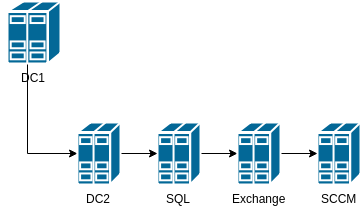
\includegraphics[width=8cm]{Netwerkdiagram.png}
\end{center}

\section{Server Requirements}

\begin{enumerate}
\item DC1
    \begin{enumerate}
    \item RAM: 2048 MB
    \item HDD: 50 GB
    \item Netwerkadapters: NAT en Internal Network (jenduf.gent)
            \begin{enumerate}
            \item NAT
            \end{enumerate}
            \begin{enumerate}
            \item IP: 192.168.1.1
            \item SN: 255.255.255.0
            \end{enumerate}
    \item OS Version: Windows Server 2016 
    \end{enumerate}
    
\clearpage

\item DC2
    \begin{enumerate}
    \item RAM: 2048 MB
    \item HDD: 50 GB
    \item Netwerkadapters: Internal Network (jenduf.gent)
            \begin{enumerate}
            \item IP: 192.168.1.2
            \item SN: 255.255.255.0
            \item DG: 192.168.1.1
            \end{enumerate}
    \item OS Version: Windows Server 2016 
    \end{enumerate}
    
\item SQL Server
    \begin{enumerate}
    \item RAM: 2048 MB
    \item HDD: 50 GB
    \item Netwerkadapters: Internal Network (jenduf.gent)
            \begin{enumerate}
            \item IP: 192.168.1.3
            \item SN: 255.255.255.0
            \item DG: 192.168.1.1
            \end{enumerate}
    \item OS Version: Windows Server 2016
    \item SQL Version: SQL Server 2013-2016
    \end{enumerate}
\item Exchange Server
    \begin{enumerate}
    \item RAM: 8096 MB
    \item HDD: 100 GB
    \item Netwerkadapters: Internal Network (jenduf.gent)
            \begin{enumerate}
            \item IP: 192.168.1.4
            \item SN: 255.255.255.0
            \item DG: 192.168.1.1
            \end{enumerate}
    \item OS Version: Windows Server 2016
    \item Exchange Version: Exchange Server 2013-2016
    \end{enumerate}
\item SCCM Server
    \begin{enumerate}
    \item RAM: 8089 MB
    \item HDD: 100 GB
    \item Netwerkadapters: Internal Network (jenduf.gent)
            \begin{enumerate}
            \item IP: 192.168.1.5
            \item SN: 255.255.255.0
            \item DG: 192.168.1.1
            \end{enumerate}
    \item OS Version: Windows Server 2016
    \item OS Version: Windows Deployment Server 2012
    \end{enumerate}
\end{enumerate}

\section{Windows Server Installatie}
\begin{center}
	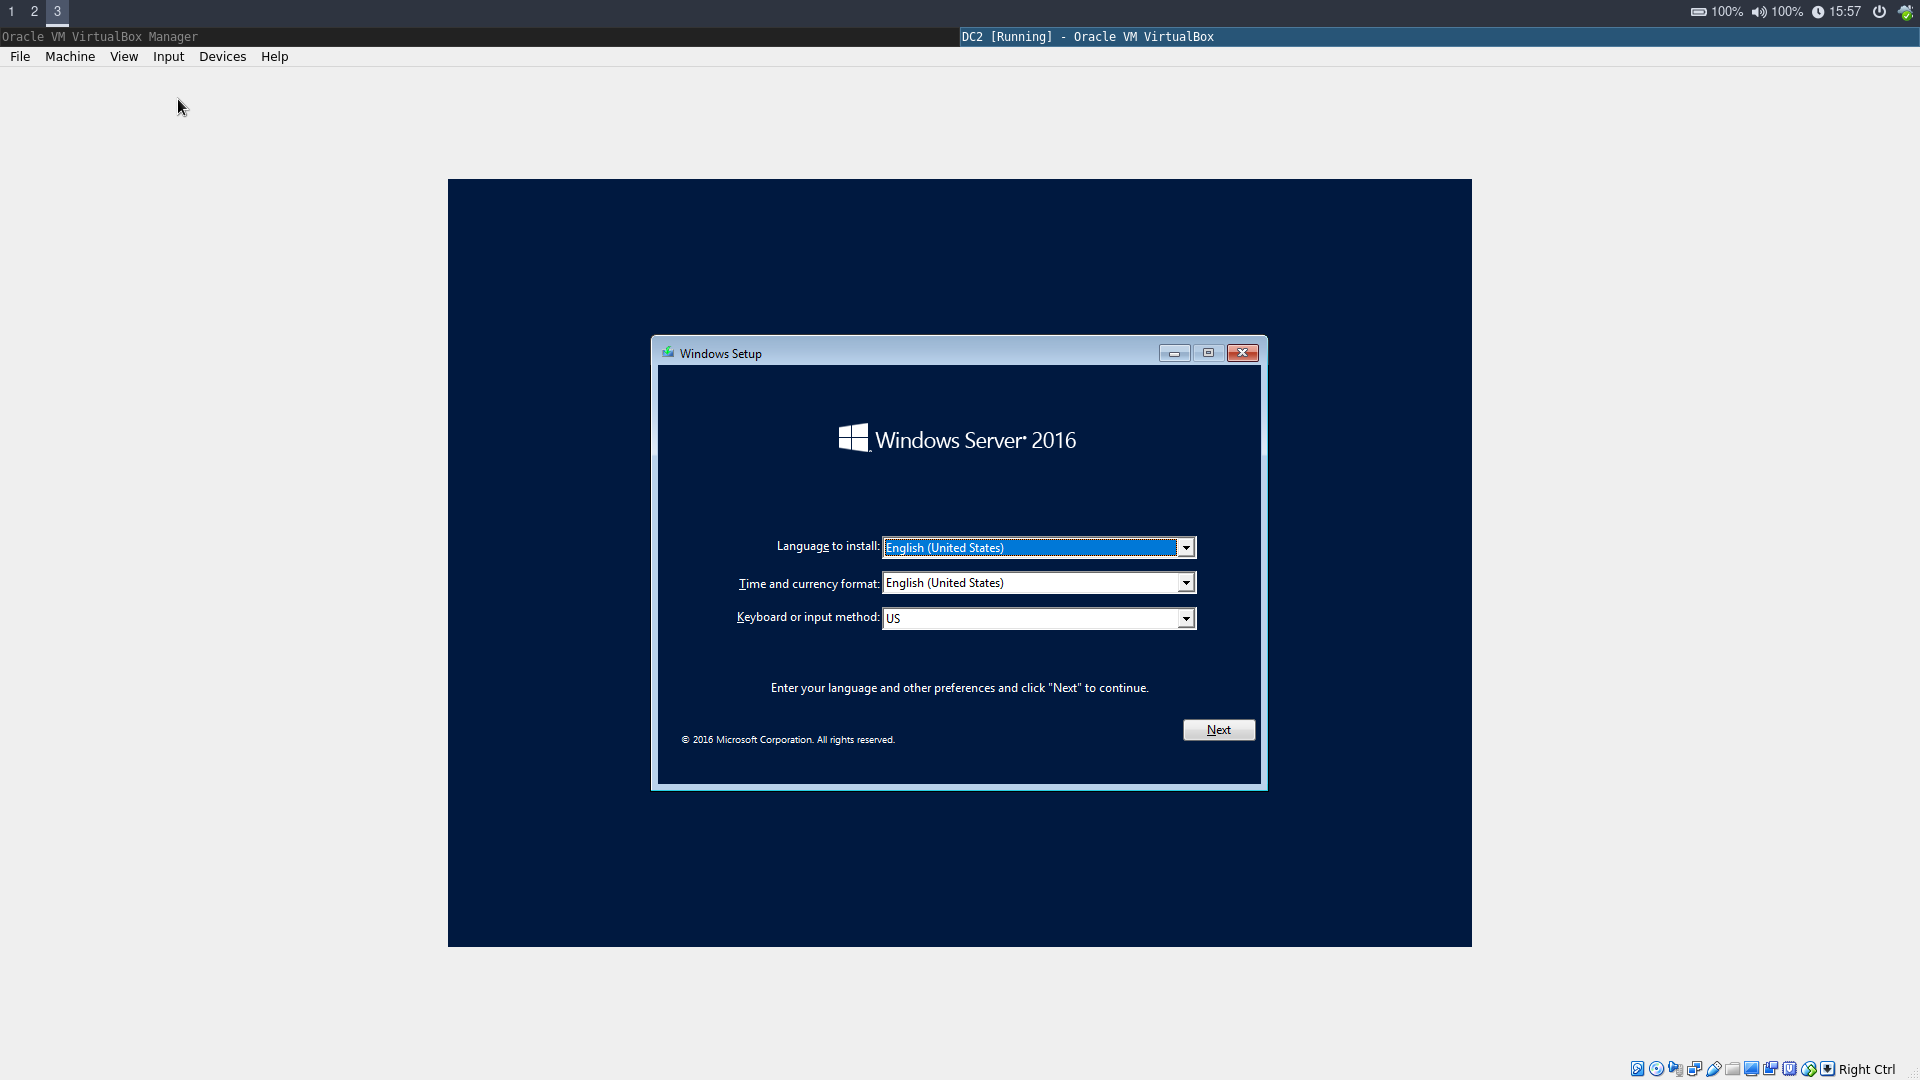
\includegraphics[width=15cm]{Pictures/Windows_Install/1542293852.png}
	Selecteer de gewenste taalinstellingen.
\end{center}
\begin{center}
	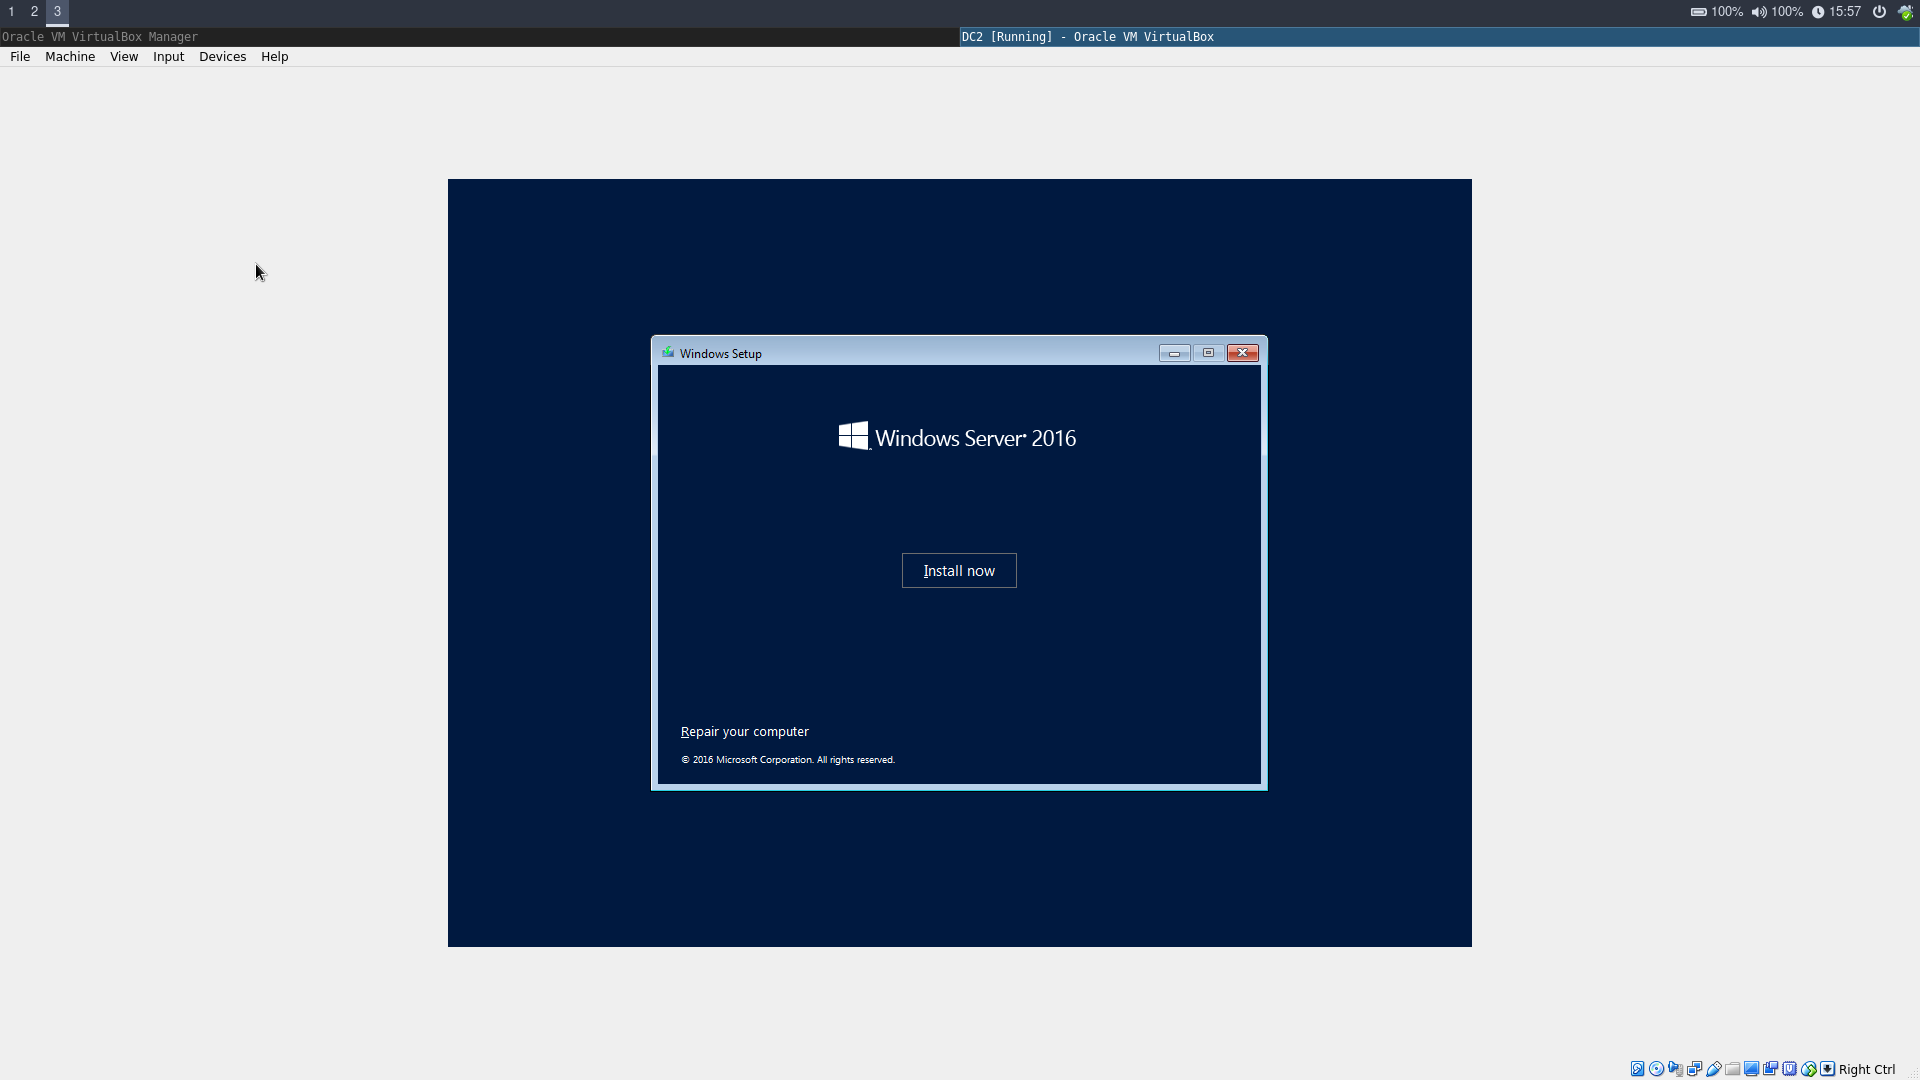
\includegraphics[width=15cm]{Pictures/Windows_Install/1542293872.png}
	
	Start de installatie.
\end{center}
\begin{center}
	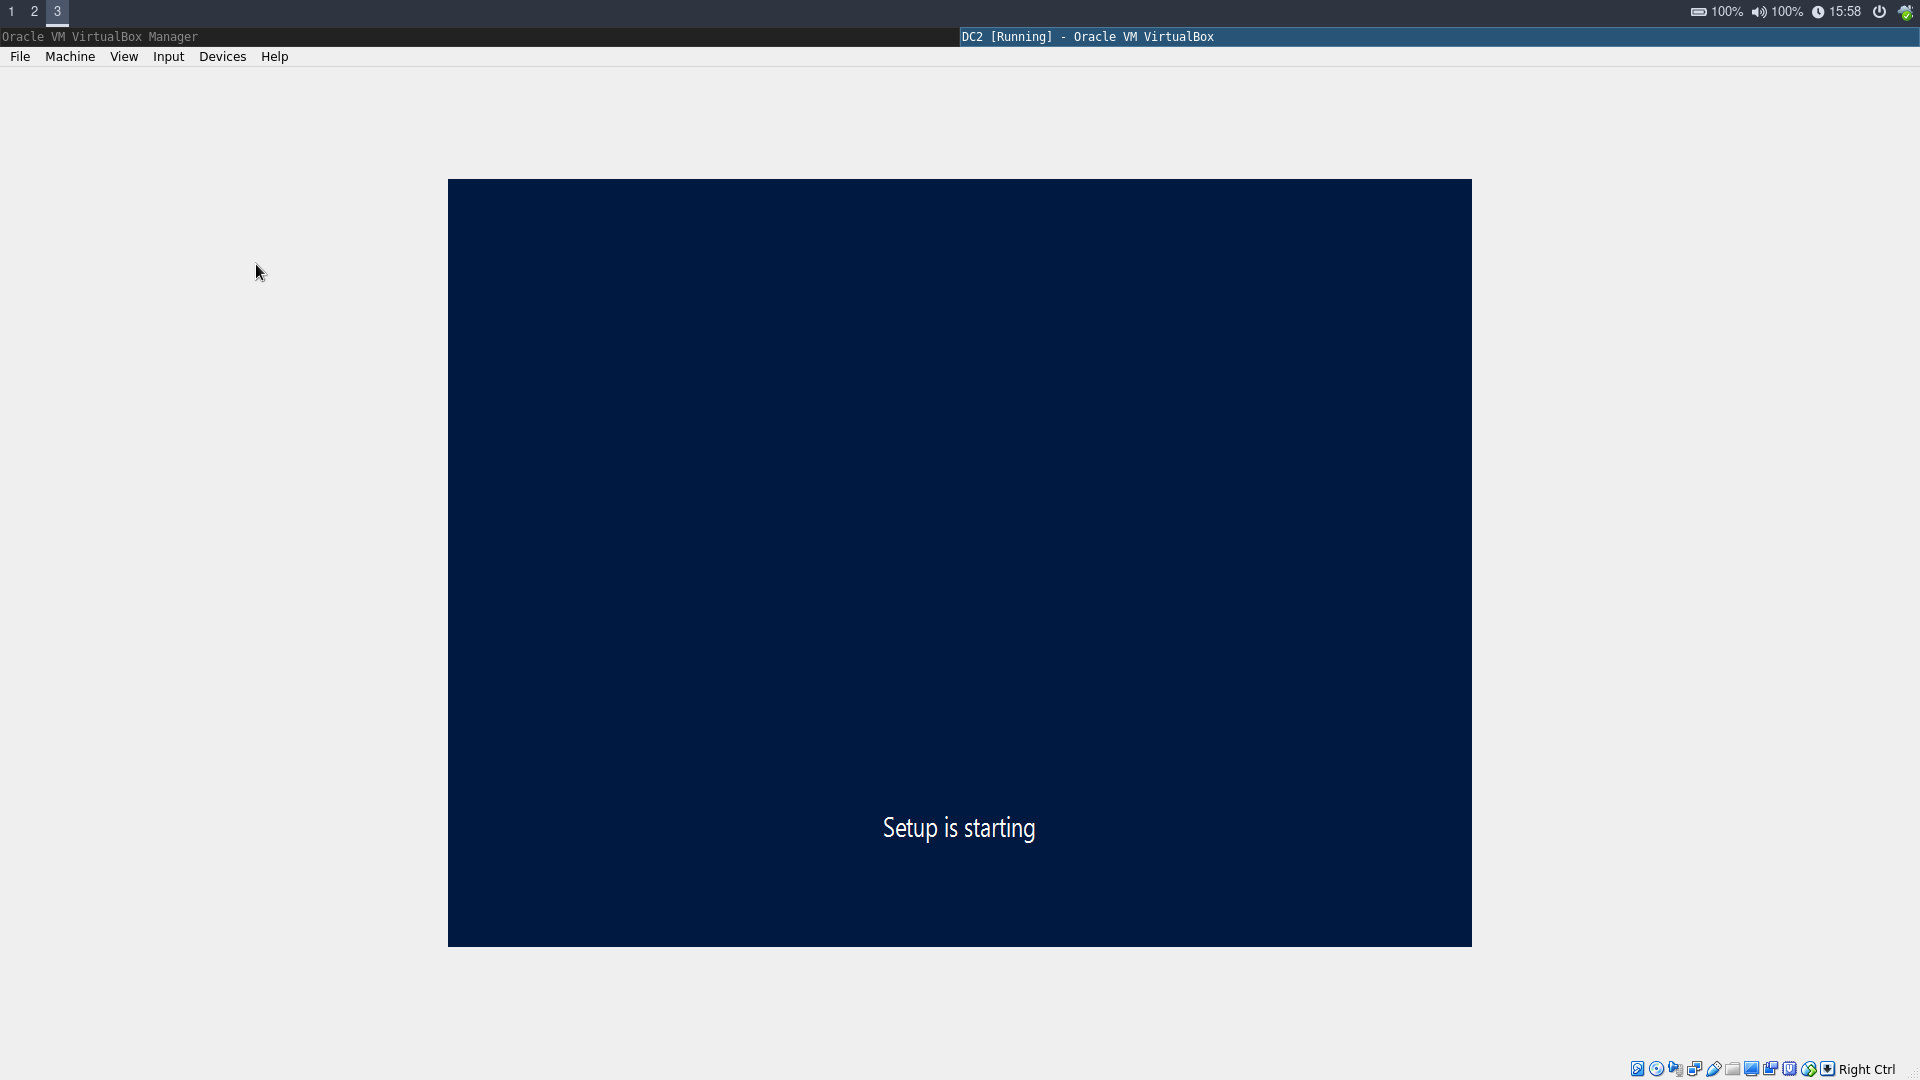
\includegraphics[width=15cm]{Pictures/Windows_Install/1542293887.png}
\end{center}
\begin{center}
	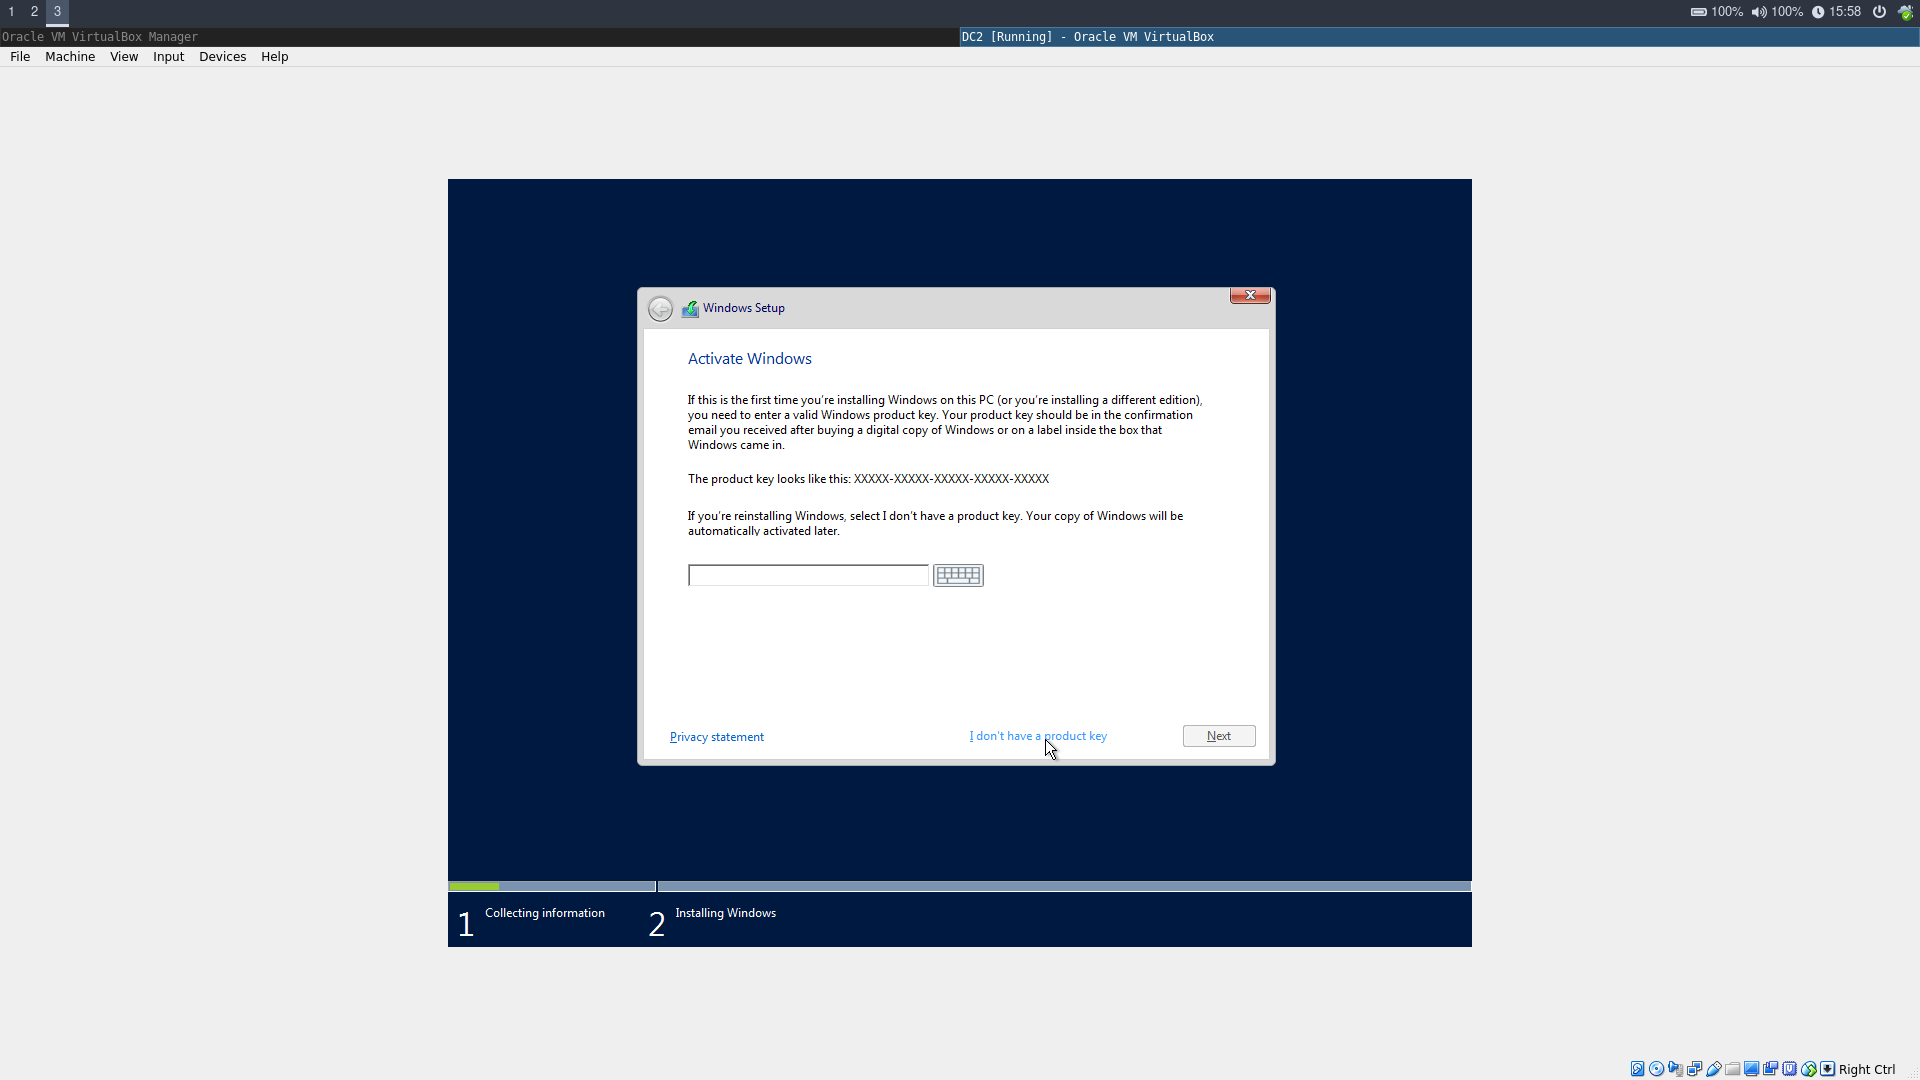
\includegraphics[width=15cm]{Pictures/Windows_Install/1542293899.png}
	
	Selecteer "I don't have a product key".
\end{center}
\begin{center}
	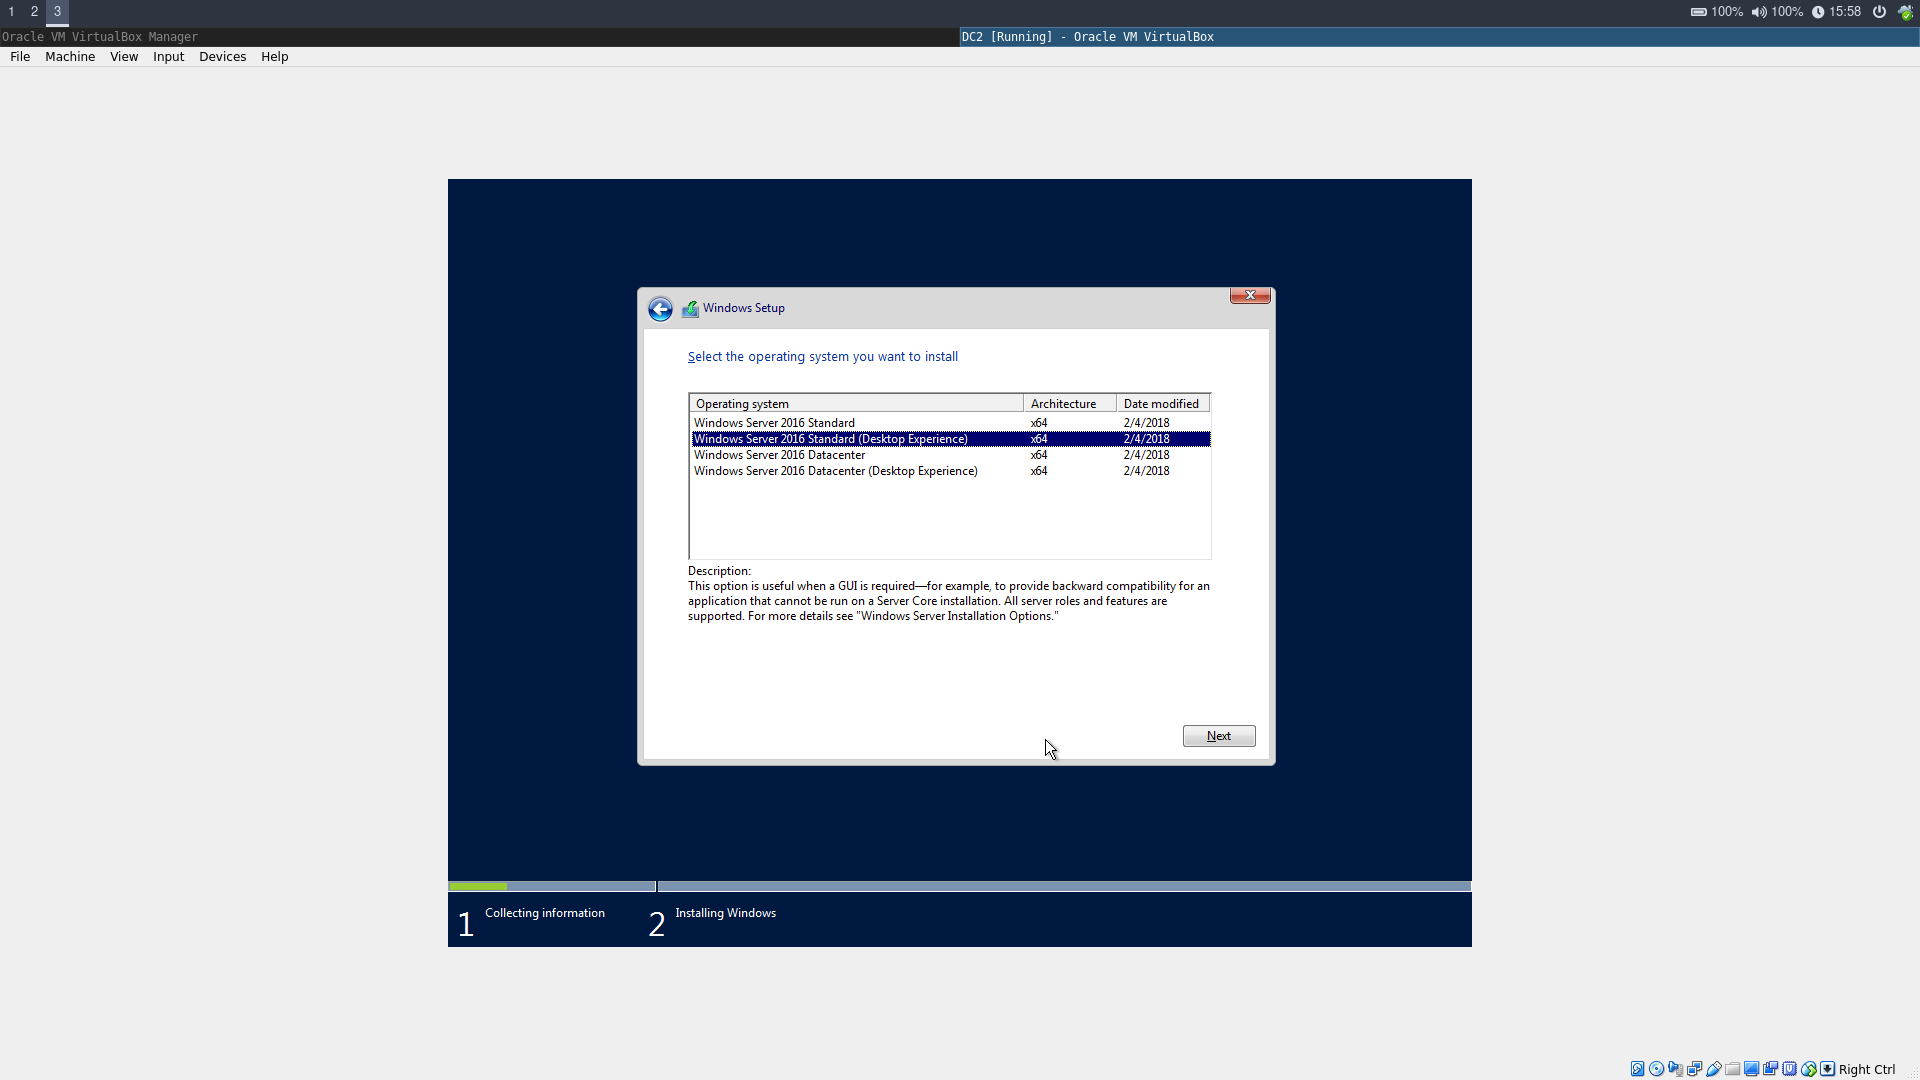
\includegraphics[width=15cm]{Pictures/Windows_Install/1542293908.png}
	
	Selecteer "Windows Server 2016 Standard (Desktop Experience)".
\end{center}
\begin{center}
	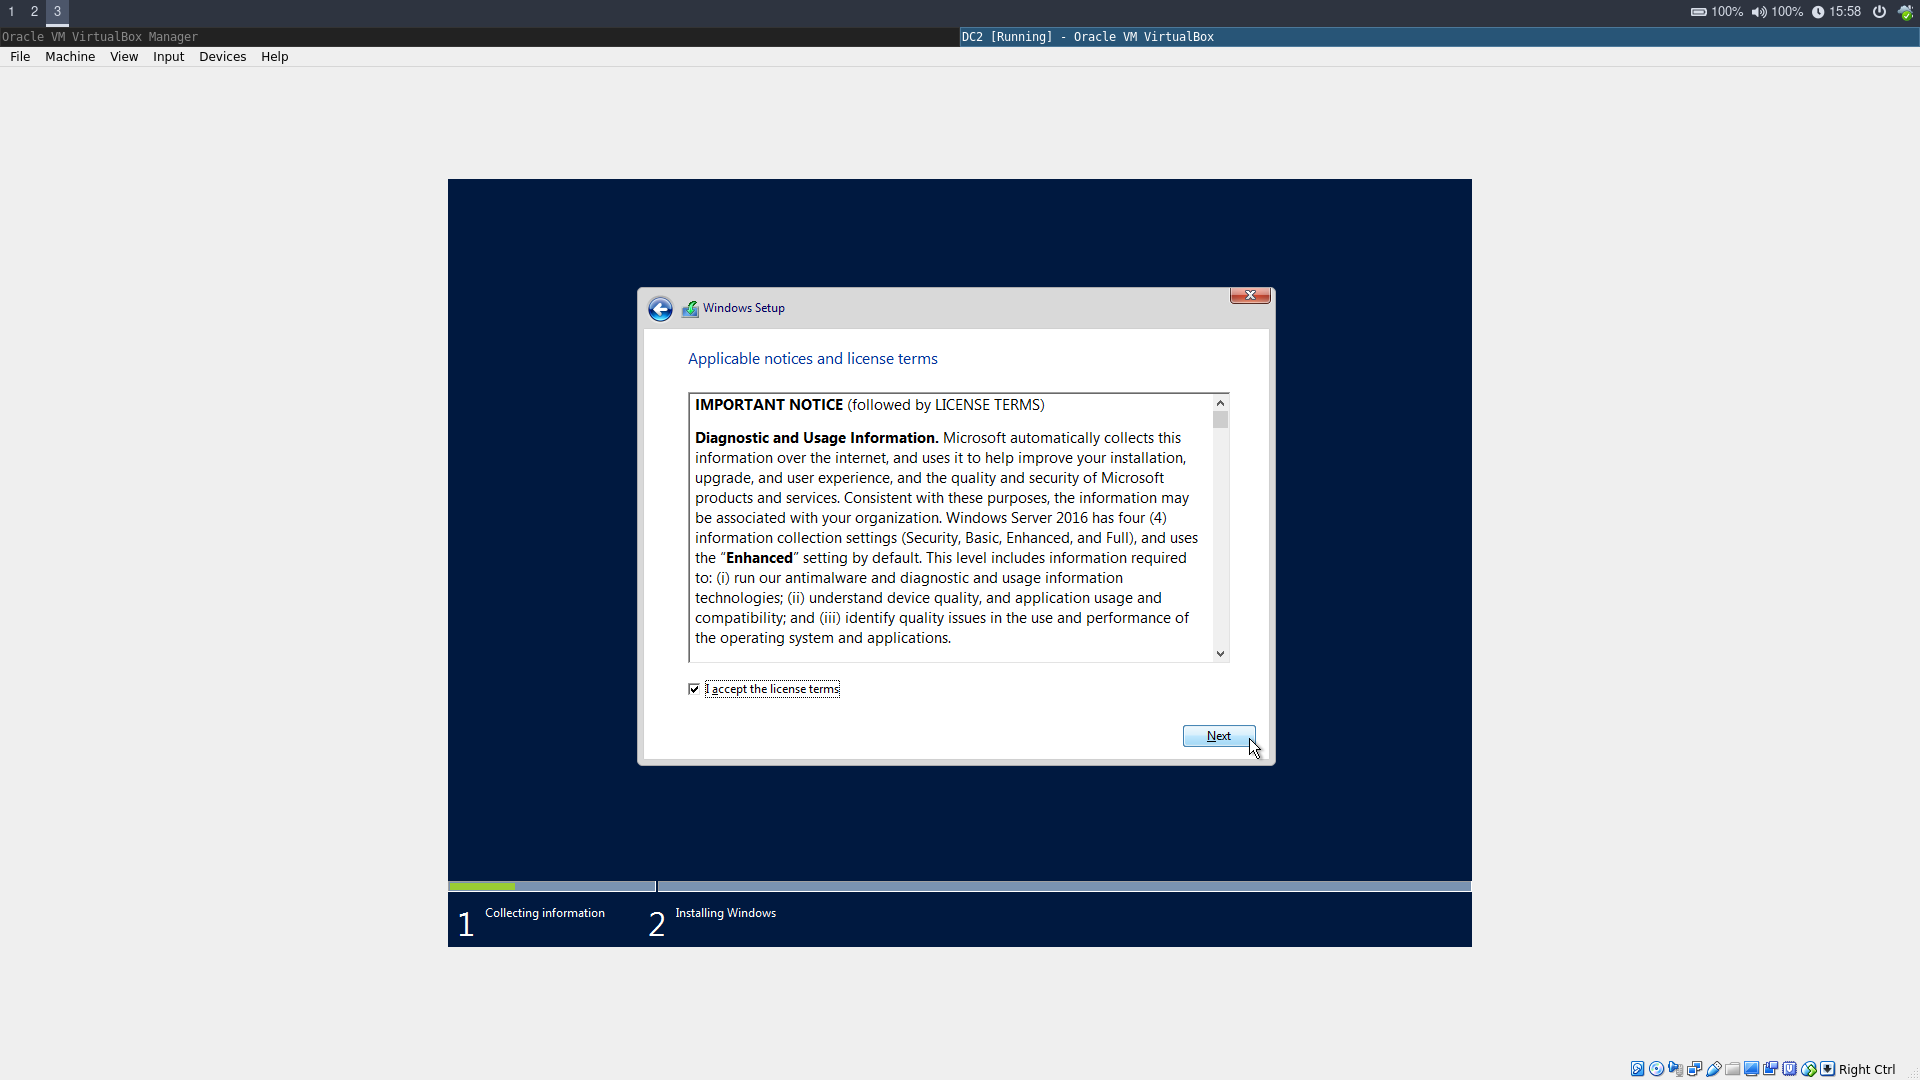
\includegraphics[width=15cm]{Pictures/Windows_Install/1542293921.png}
	
	Ga akkoord met de gebruiksvoorwaarden.
\end{center}
\begin{center}
	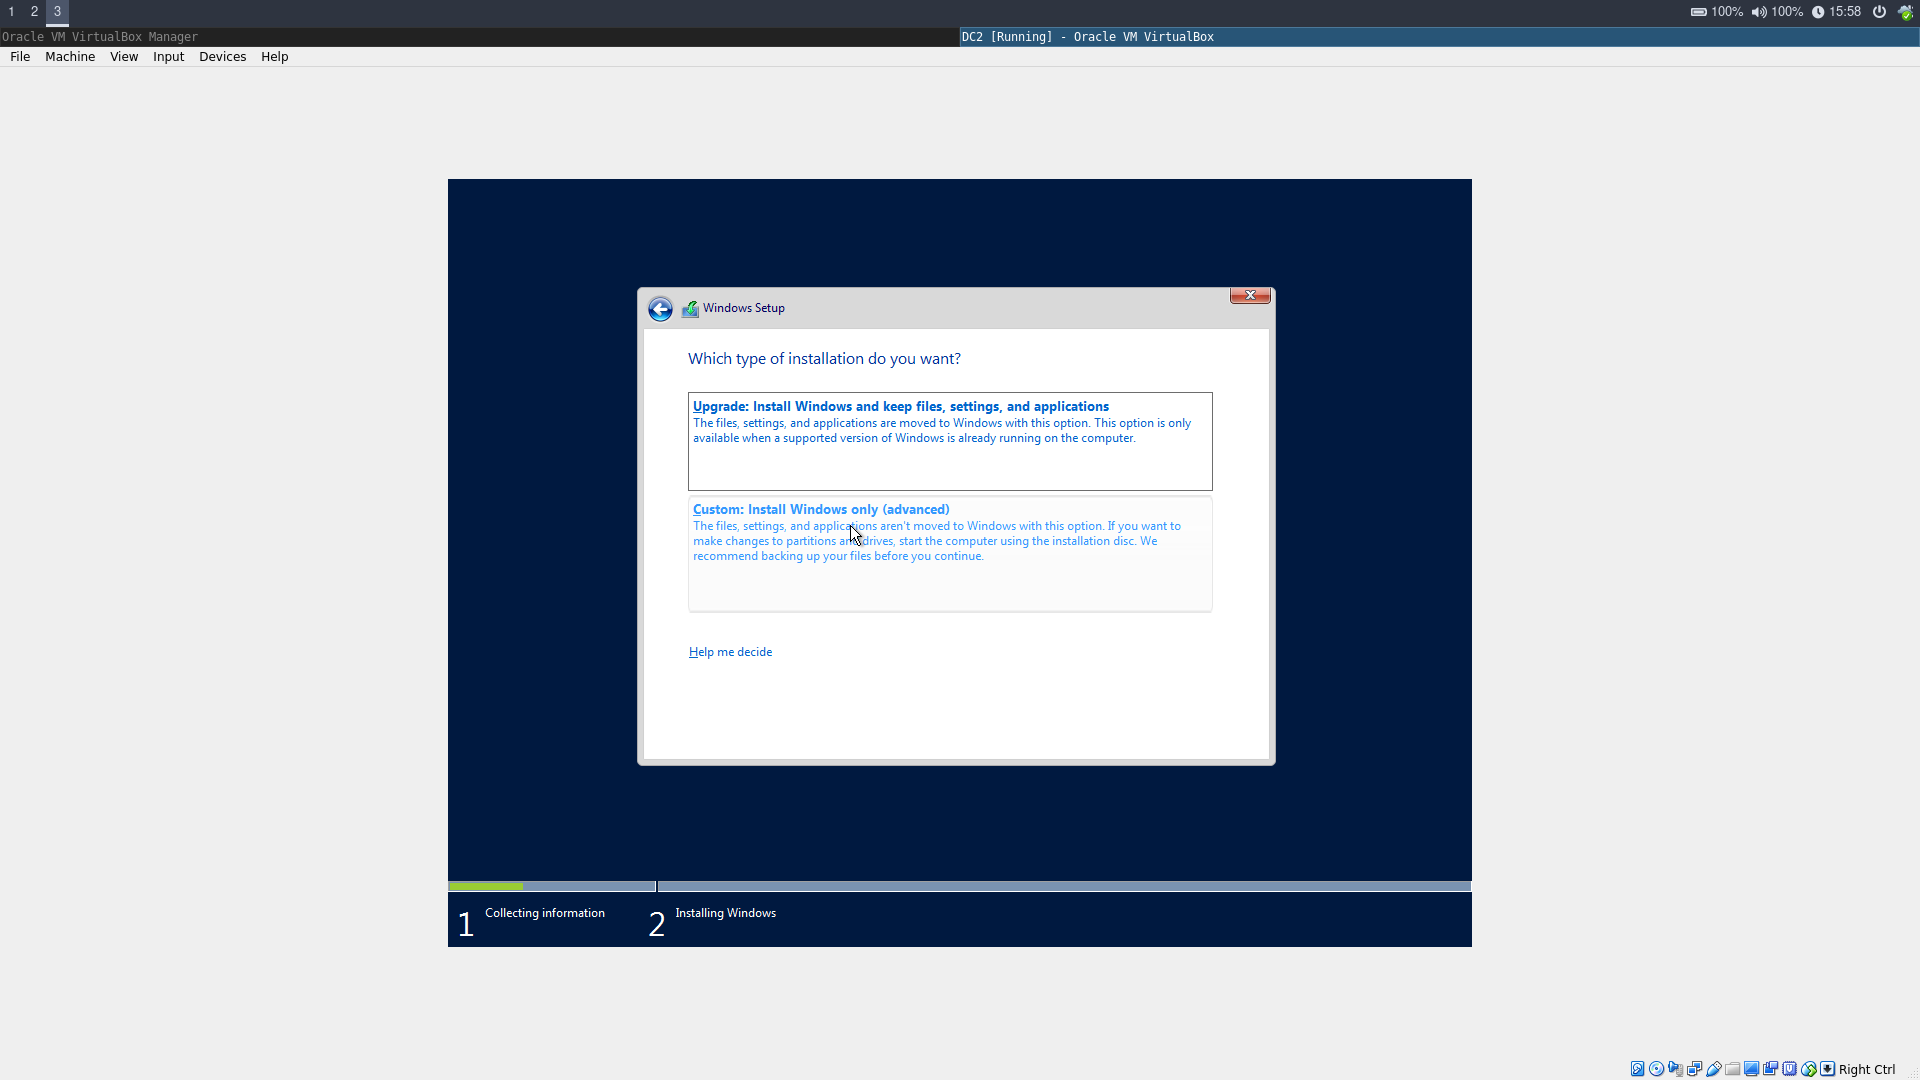
\includegraphics[width=15cm]{Pictures/Windows_Install/1542293929.png}
	
	Selecteer "Costum: Install Windows only (Advanced)".
\end{center}
\begin{center}
	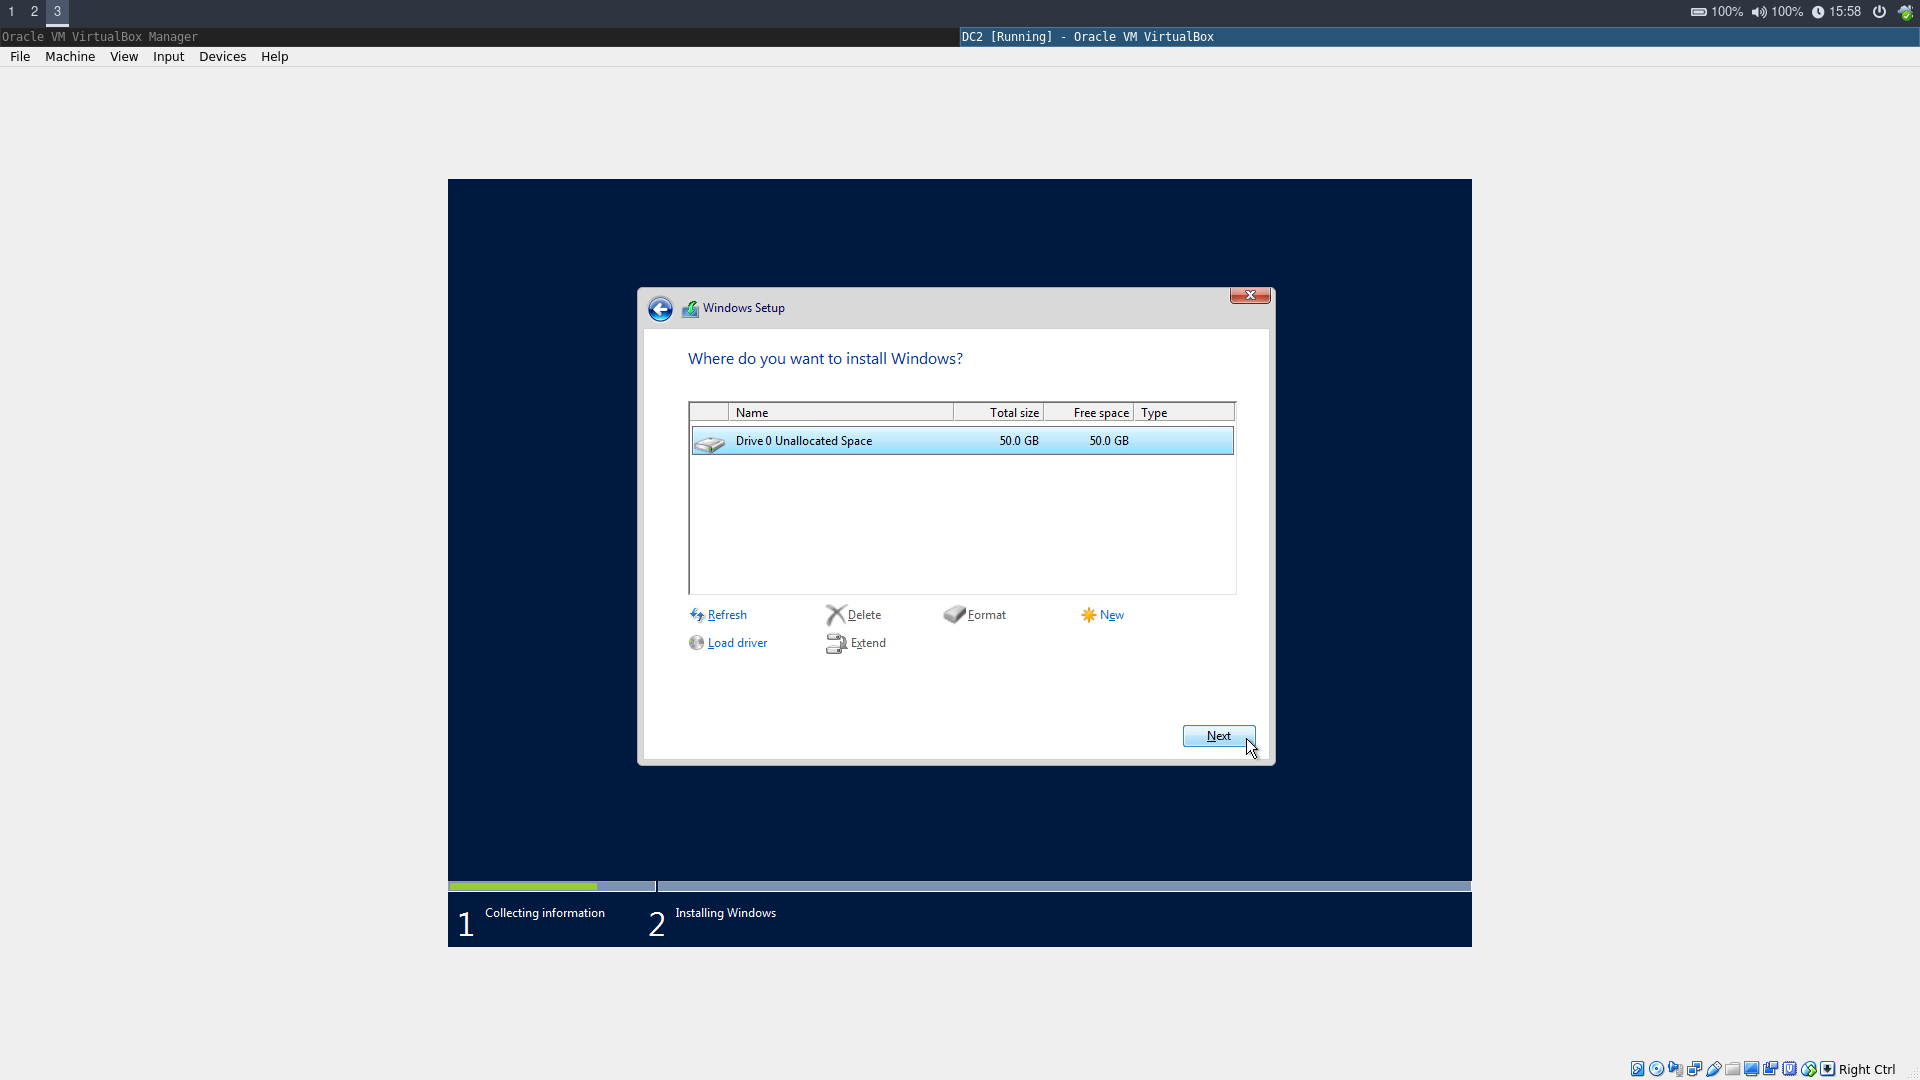
\includegraphics[width=15cm]{Pictures/Windows_Install/1542293934.png}
	
	Ga verder.
\end{center}
\begin{center}
	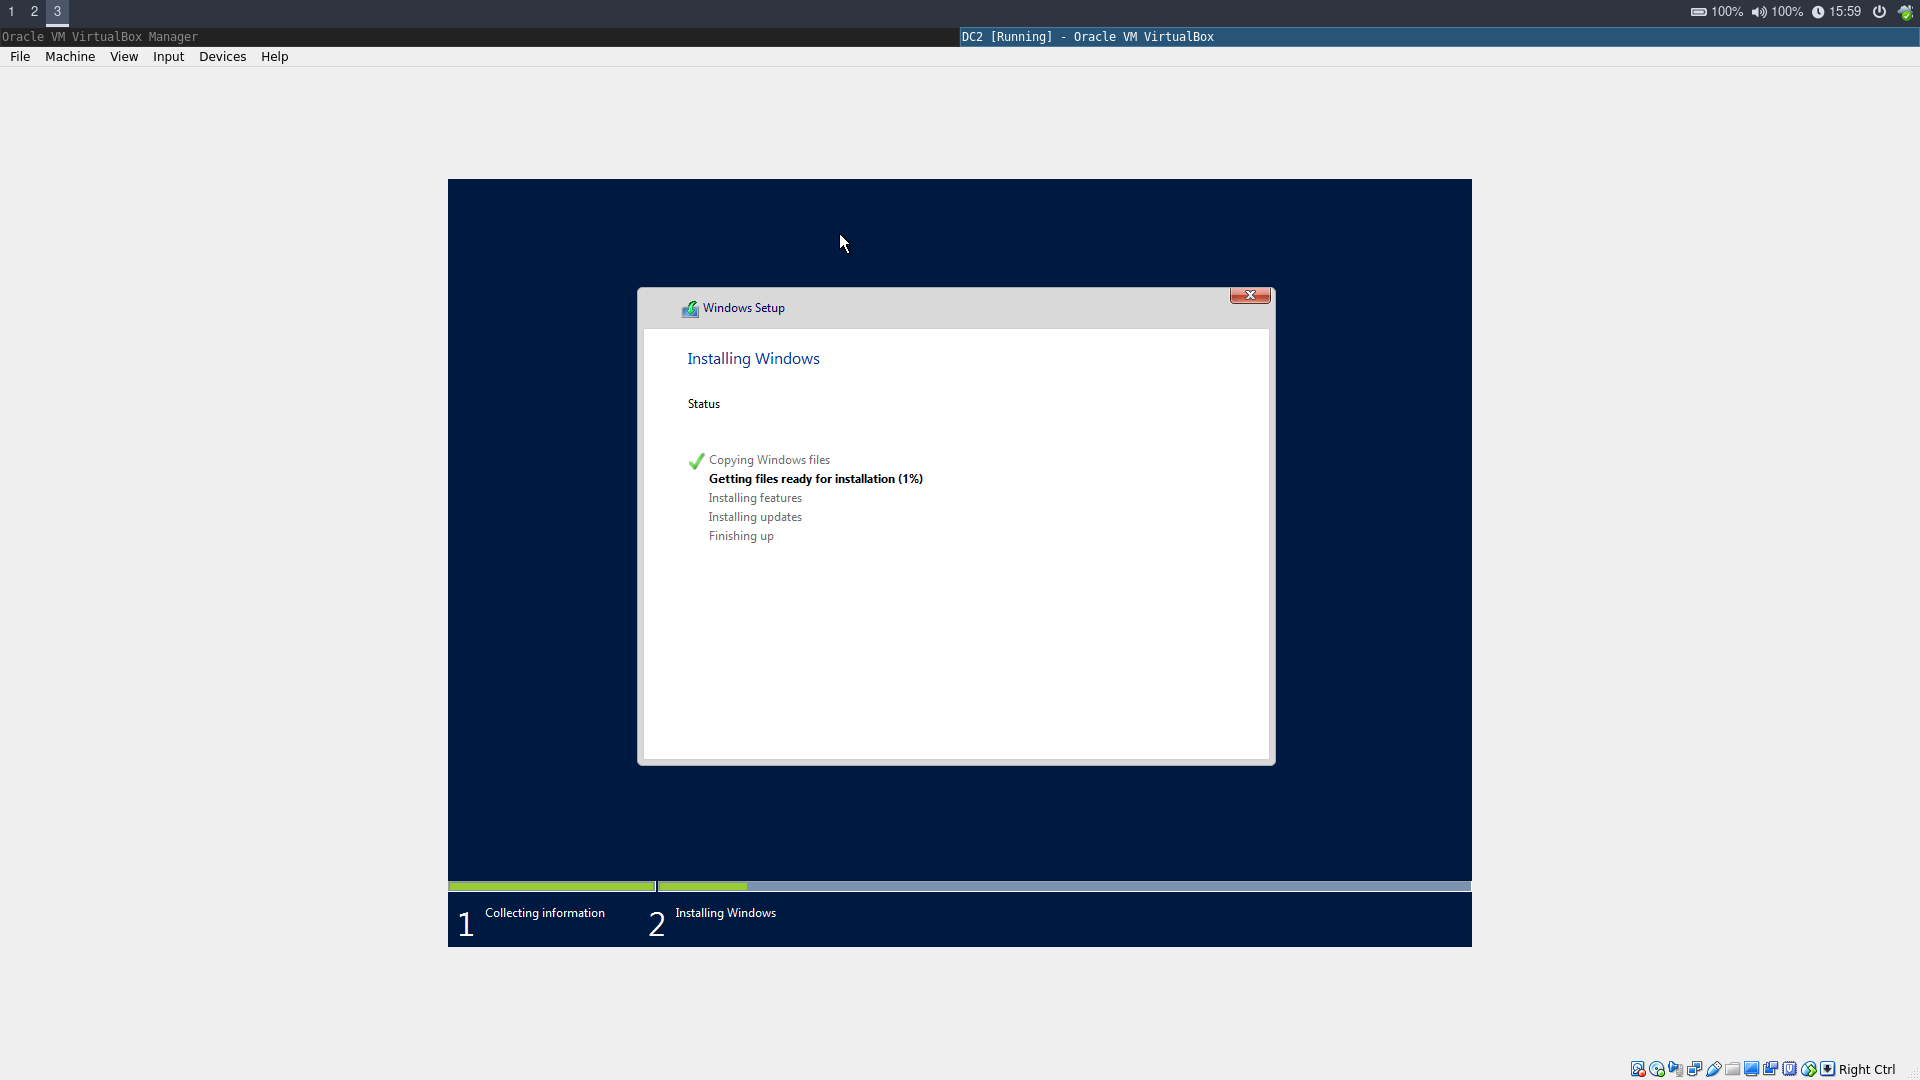
\includegraphics[width=15cm]{Pictures/Windows_Install/1542293945.png}
\end{center}
\subsection{Server Hernoemen}
\begin{center}
	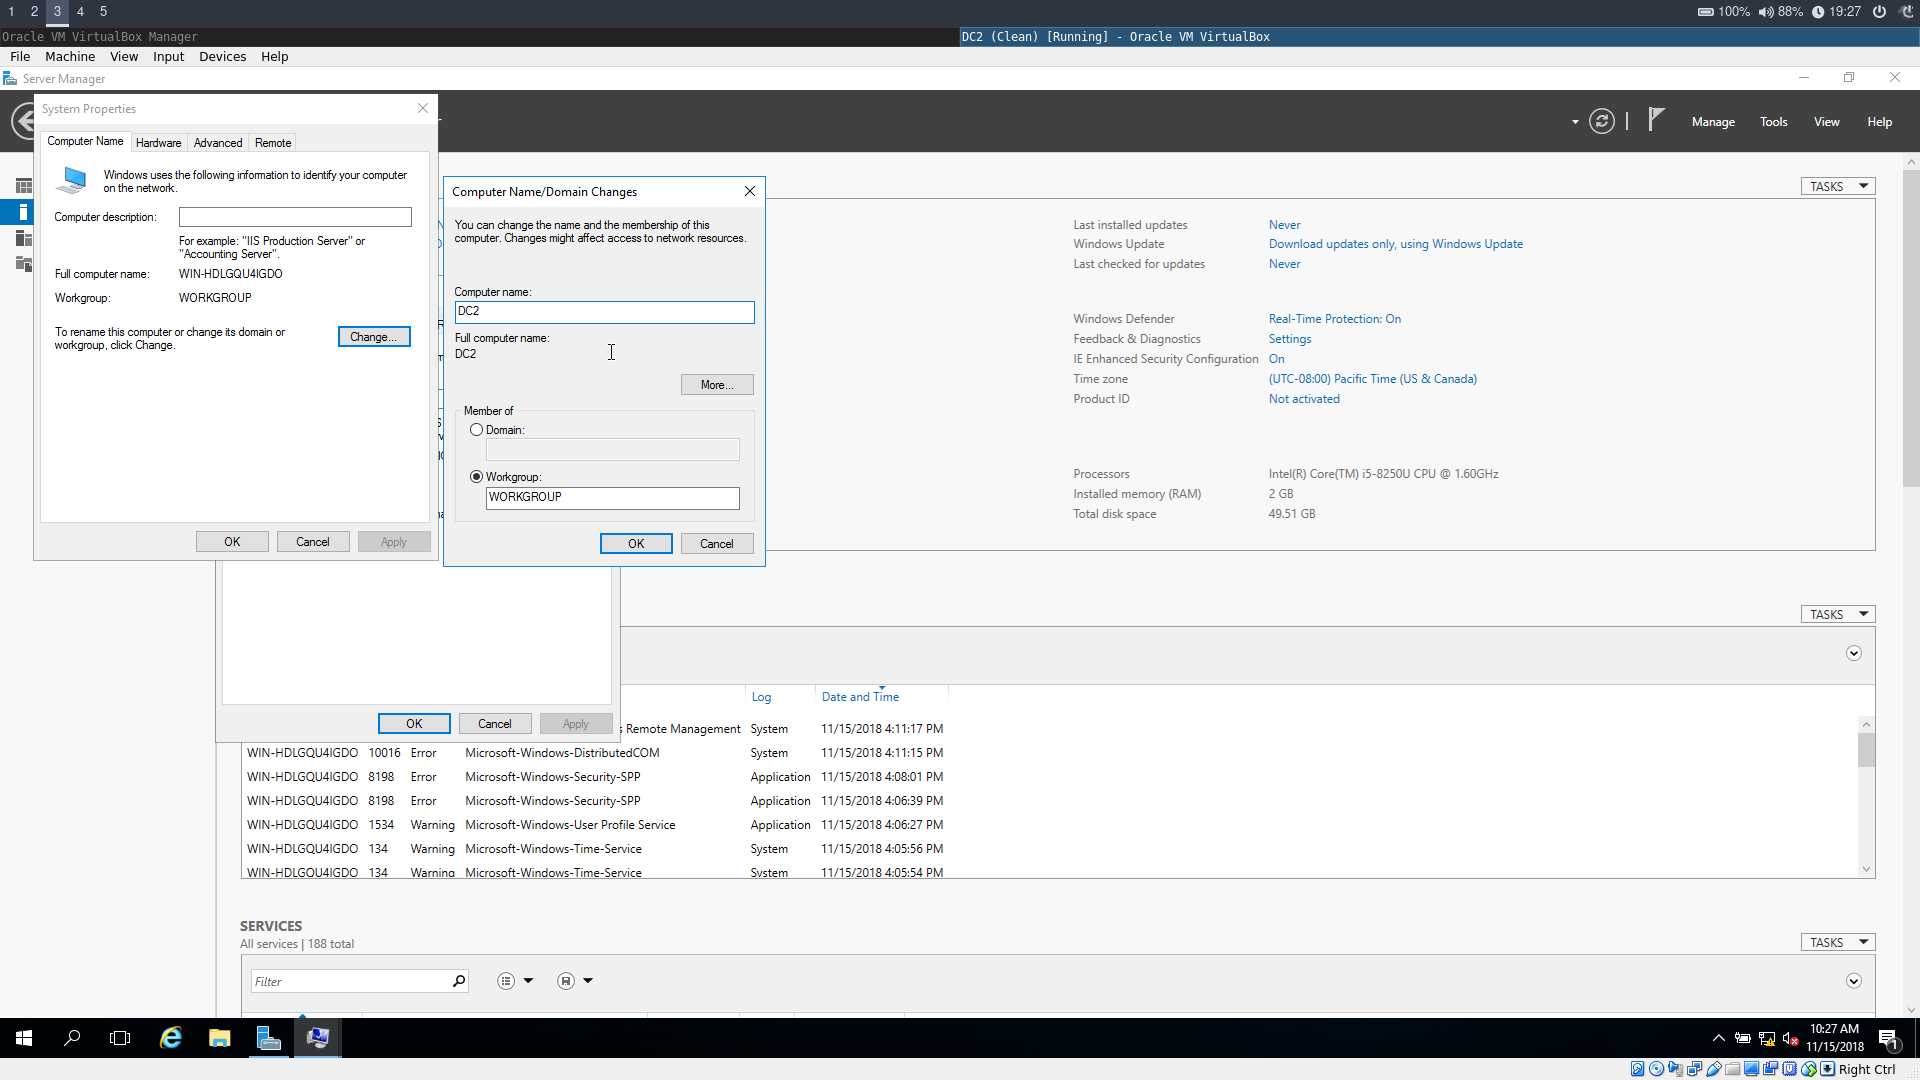
\includegraphics[width=15cm]{Pictures/DC2/Basisconfiguratie/1542306425.png}
\end{center}
\subsection{IP Instellingen}
\begin{center}
	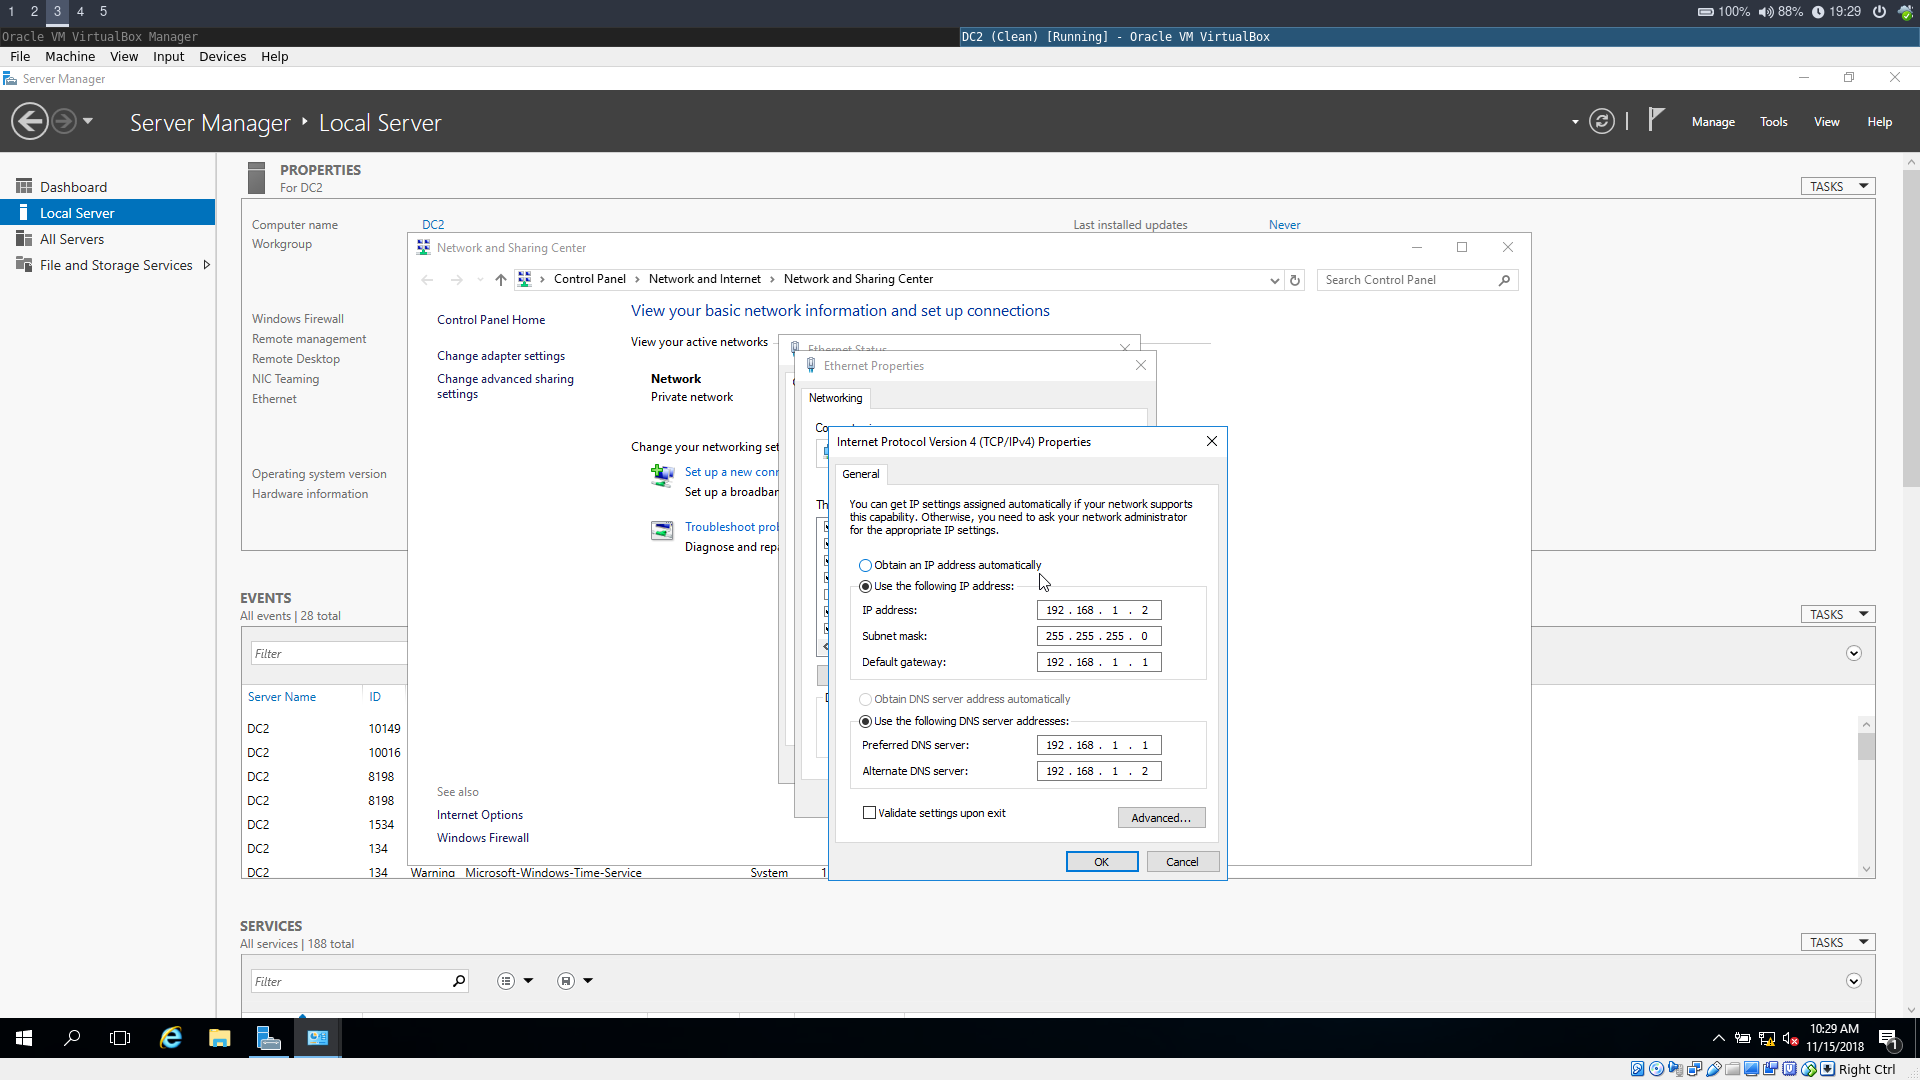
\includegraphics[width=15cm]{Pictures/DC2/Basisconfiguratie/1542306587.png}
\end{center}
\subsection{Toevoegen aan het domein}
\begin{center}
	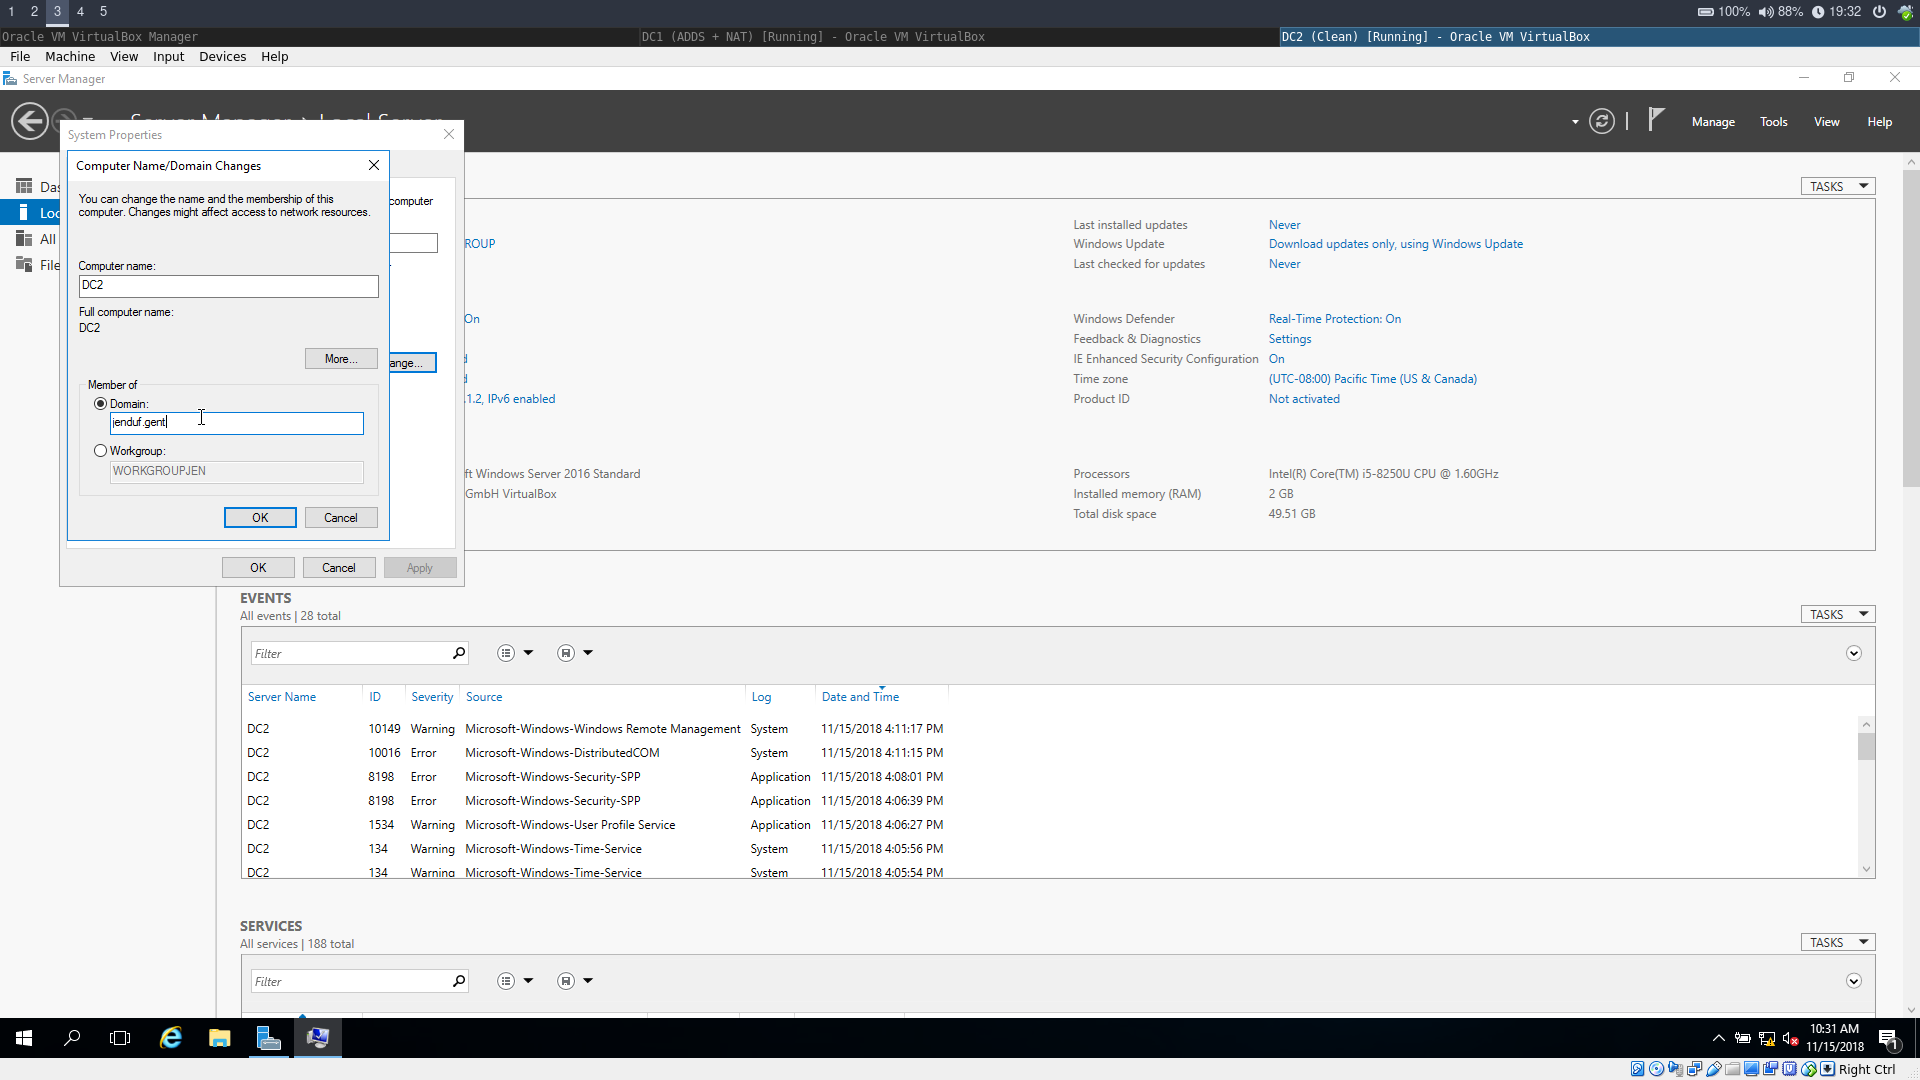
\includegraphics[width=15cm]{Pictures/DC2/Basisconfiguratie/1542306751.png}
	
	Geef als domein jenduf.gent in.
\end{center}
\begin{center}
	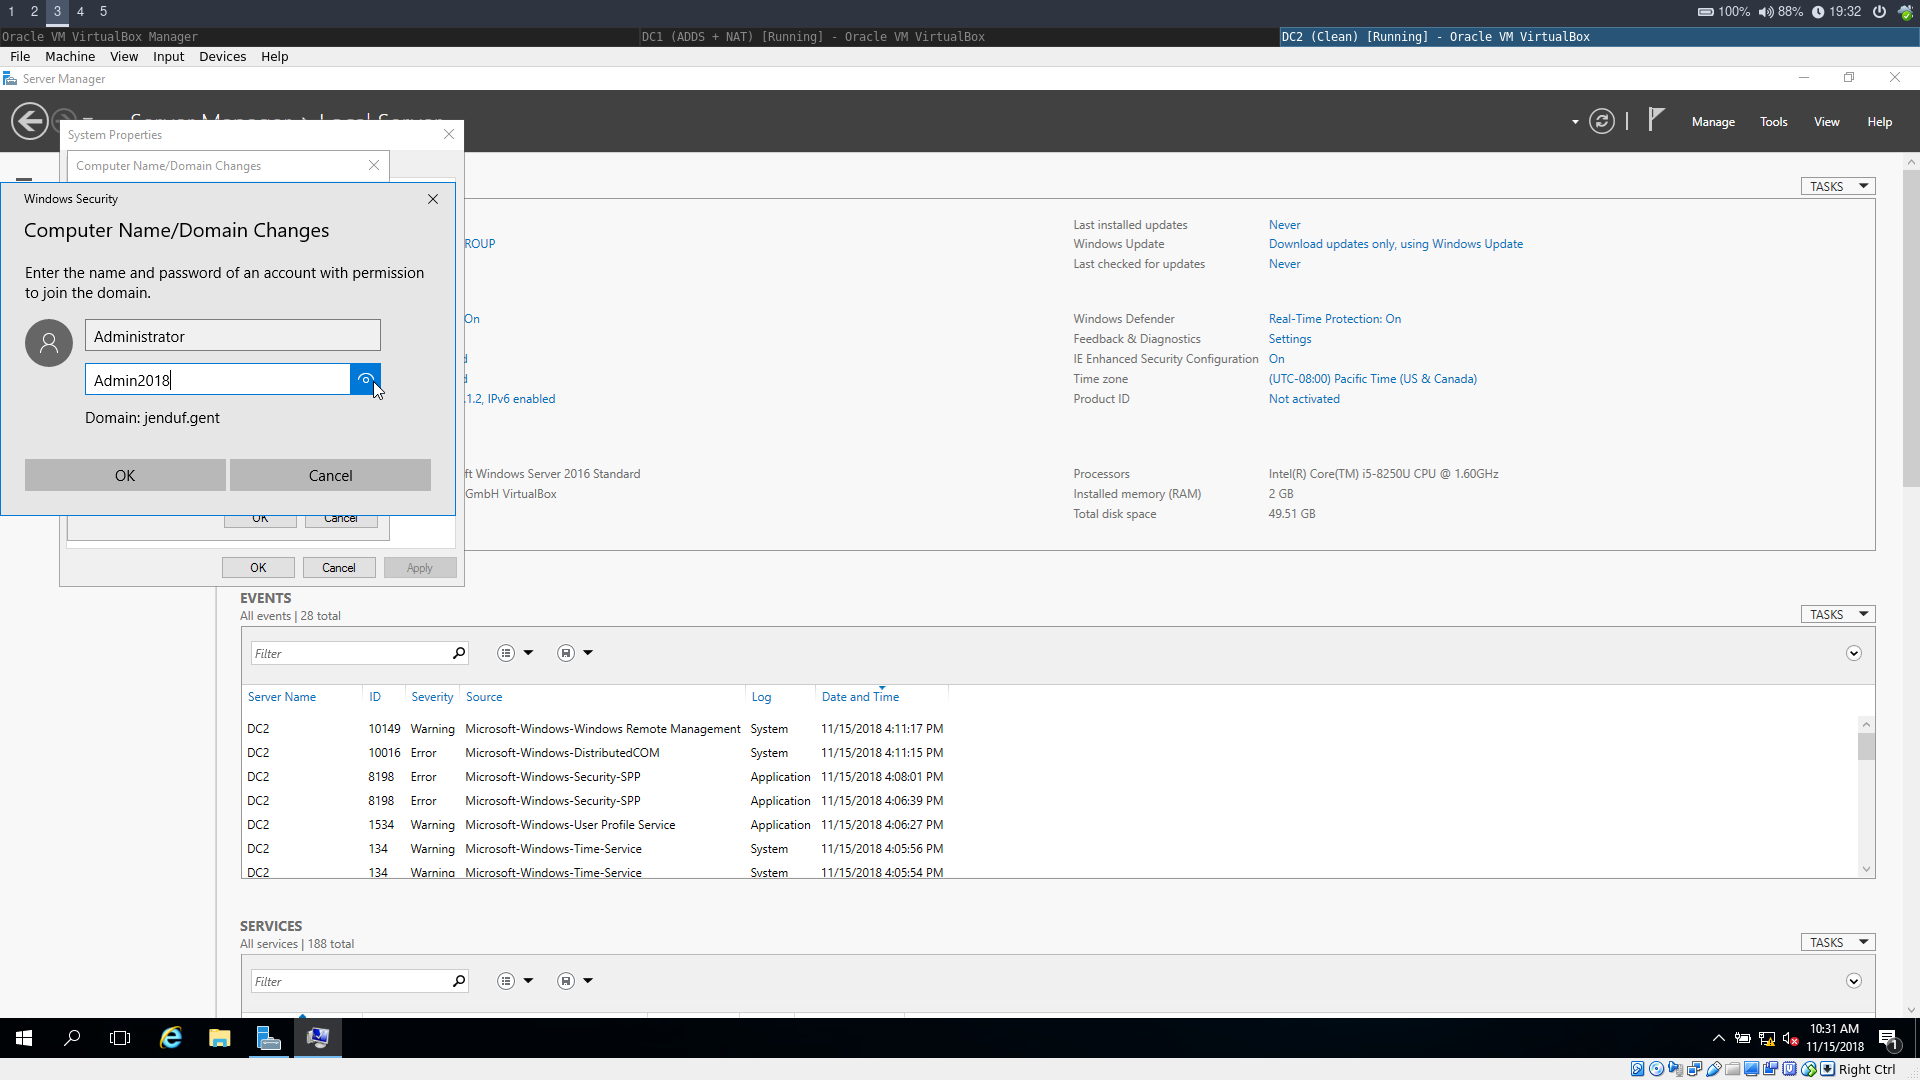
\includegraphics[width=15cm]{Pictures/DC2/Basisconfiguratie/1542306762.png}
	
	Geem gebruikersnaam "Administrator" in en paswoord "Admin2018".
\end{center}
\begin{center}
	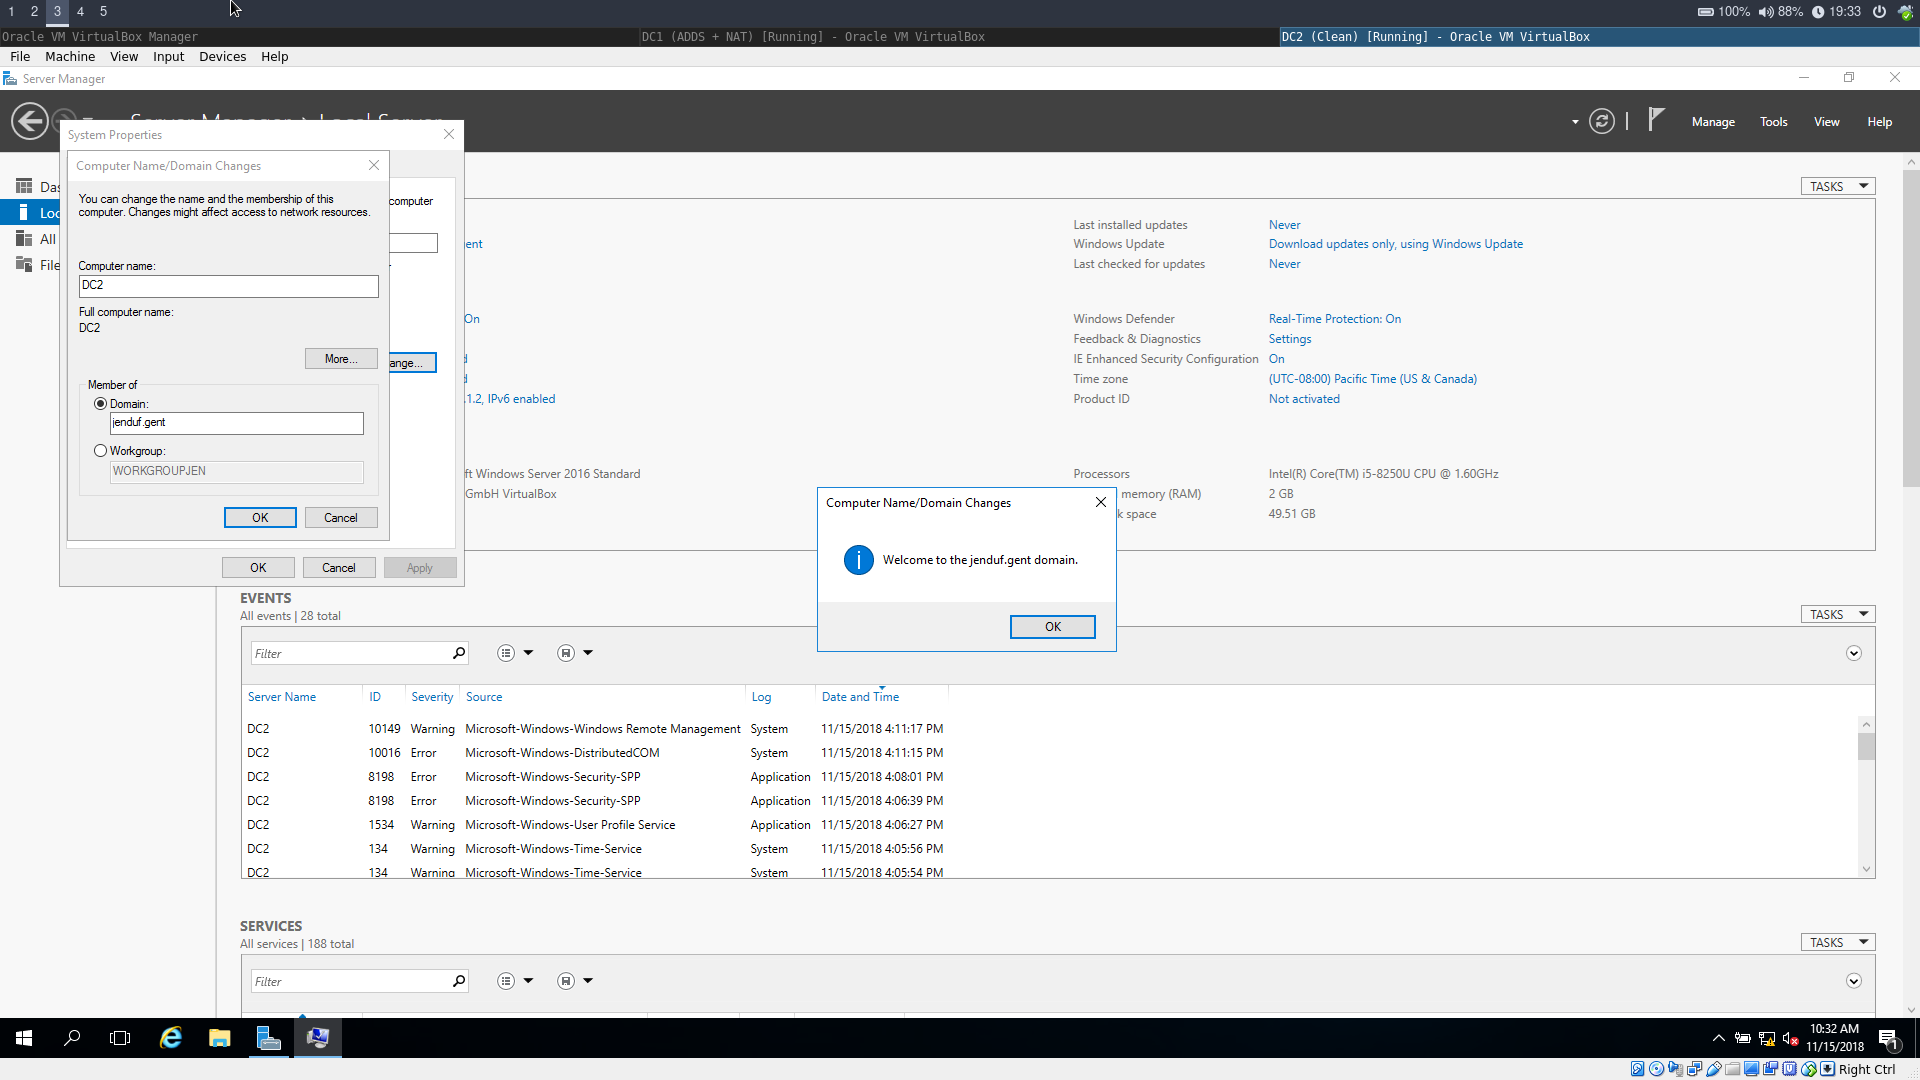
\includegraphics[width=15cm]{Pictures/DC2/Basisconfiguratie/1542306780.png}
	
	De connectie is geslaagd bij het weergeven van volgende boodschap.
	
\end{center}


\section{Installatie ADDS}
\begin{center}
	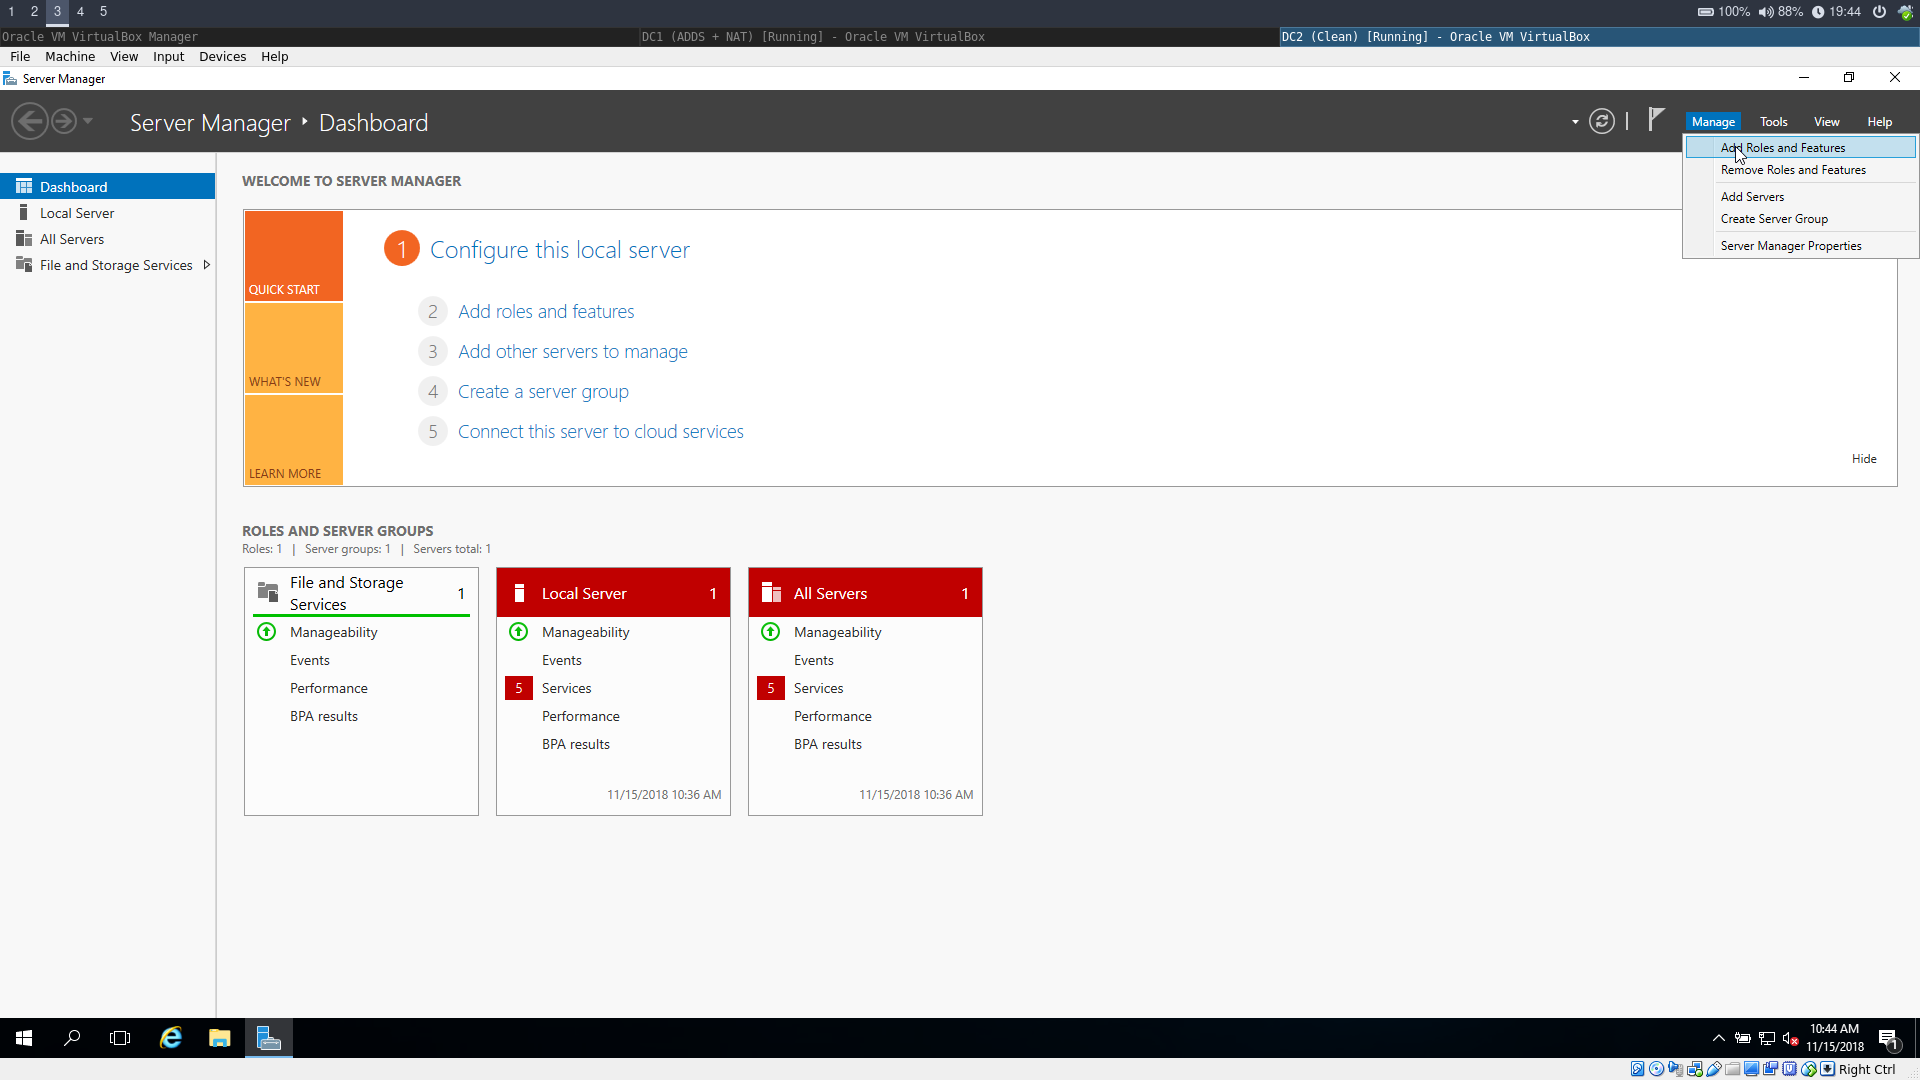
\includegraphics[width=15cm]{Pictures/DC2/ADDS/1542307480.png}
	
	Voeg een nieuwe rol toe.
\end{center}
\begin{center}
	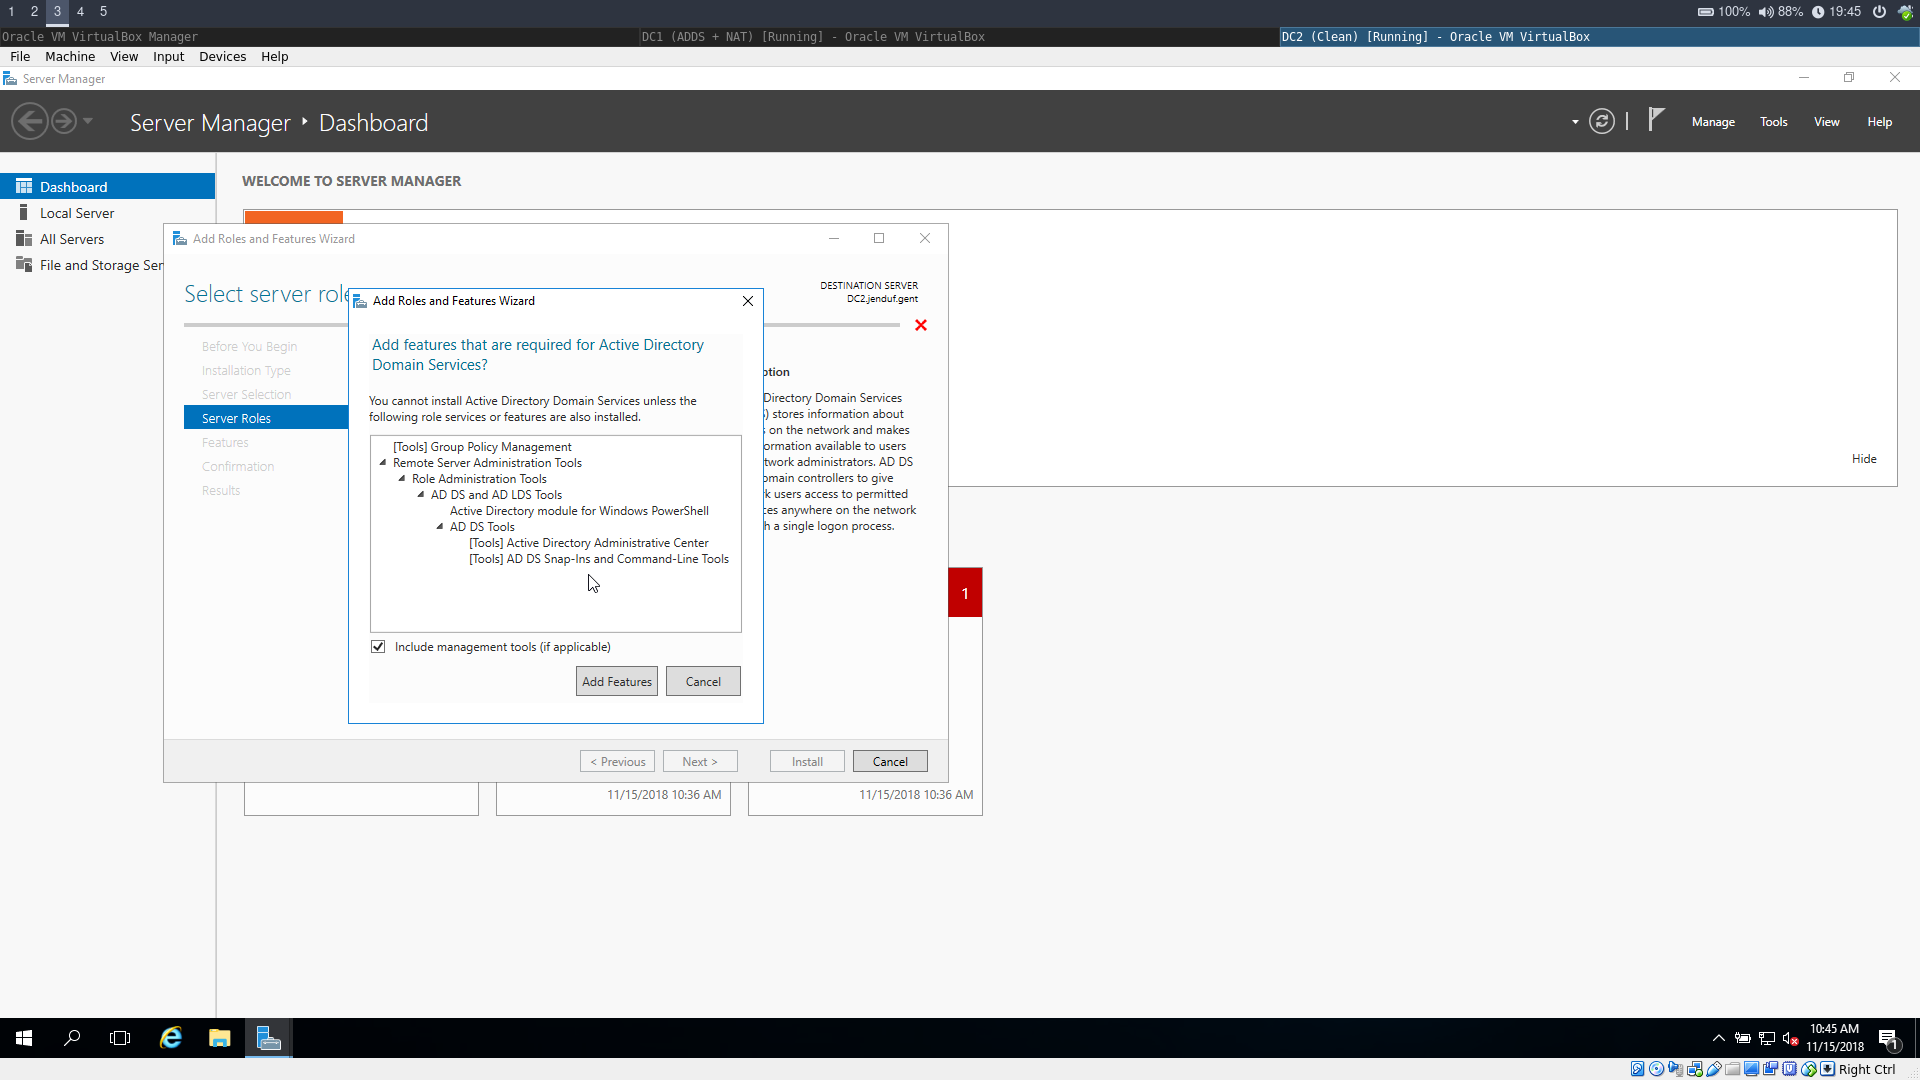
\includegraphics[width=15cm]{Pictures/DC2/ADDS/1542307514.png}
	
	Selecteer "Active Domain Directory Service".
\end{center}
\begin{center}
	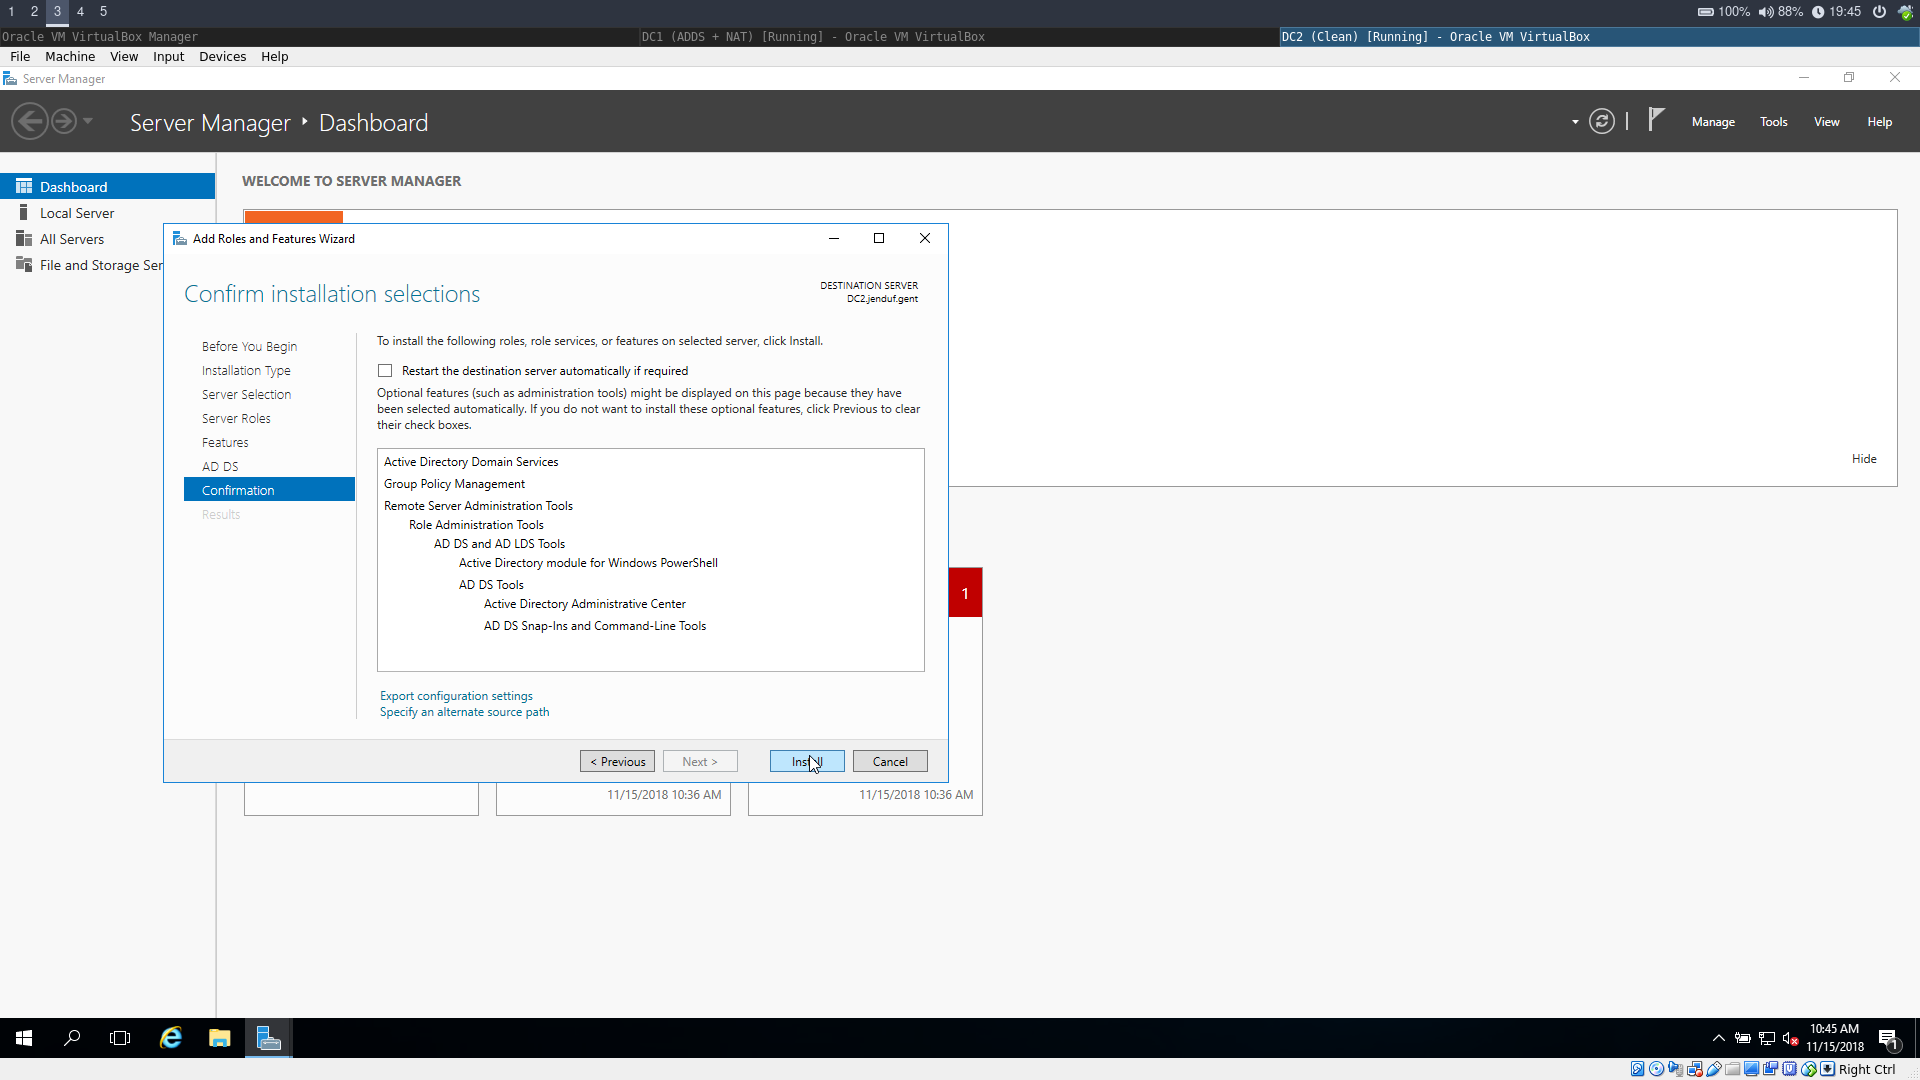
\includegraphics[width=15cm]{Pictures/DC2/ADDS/1542307525.png}
	
	Volg de installatiewizard.
\end{center}
\begin{center}
	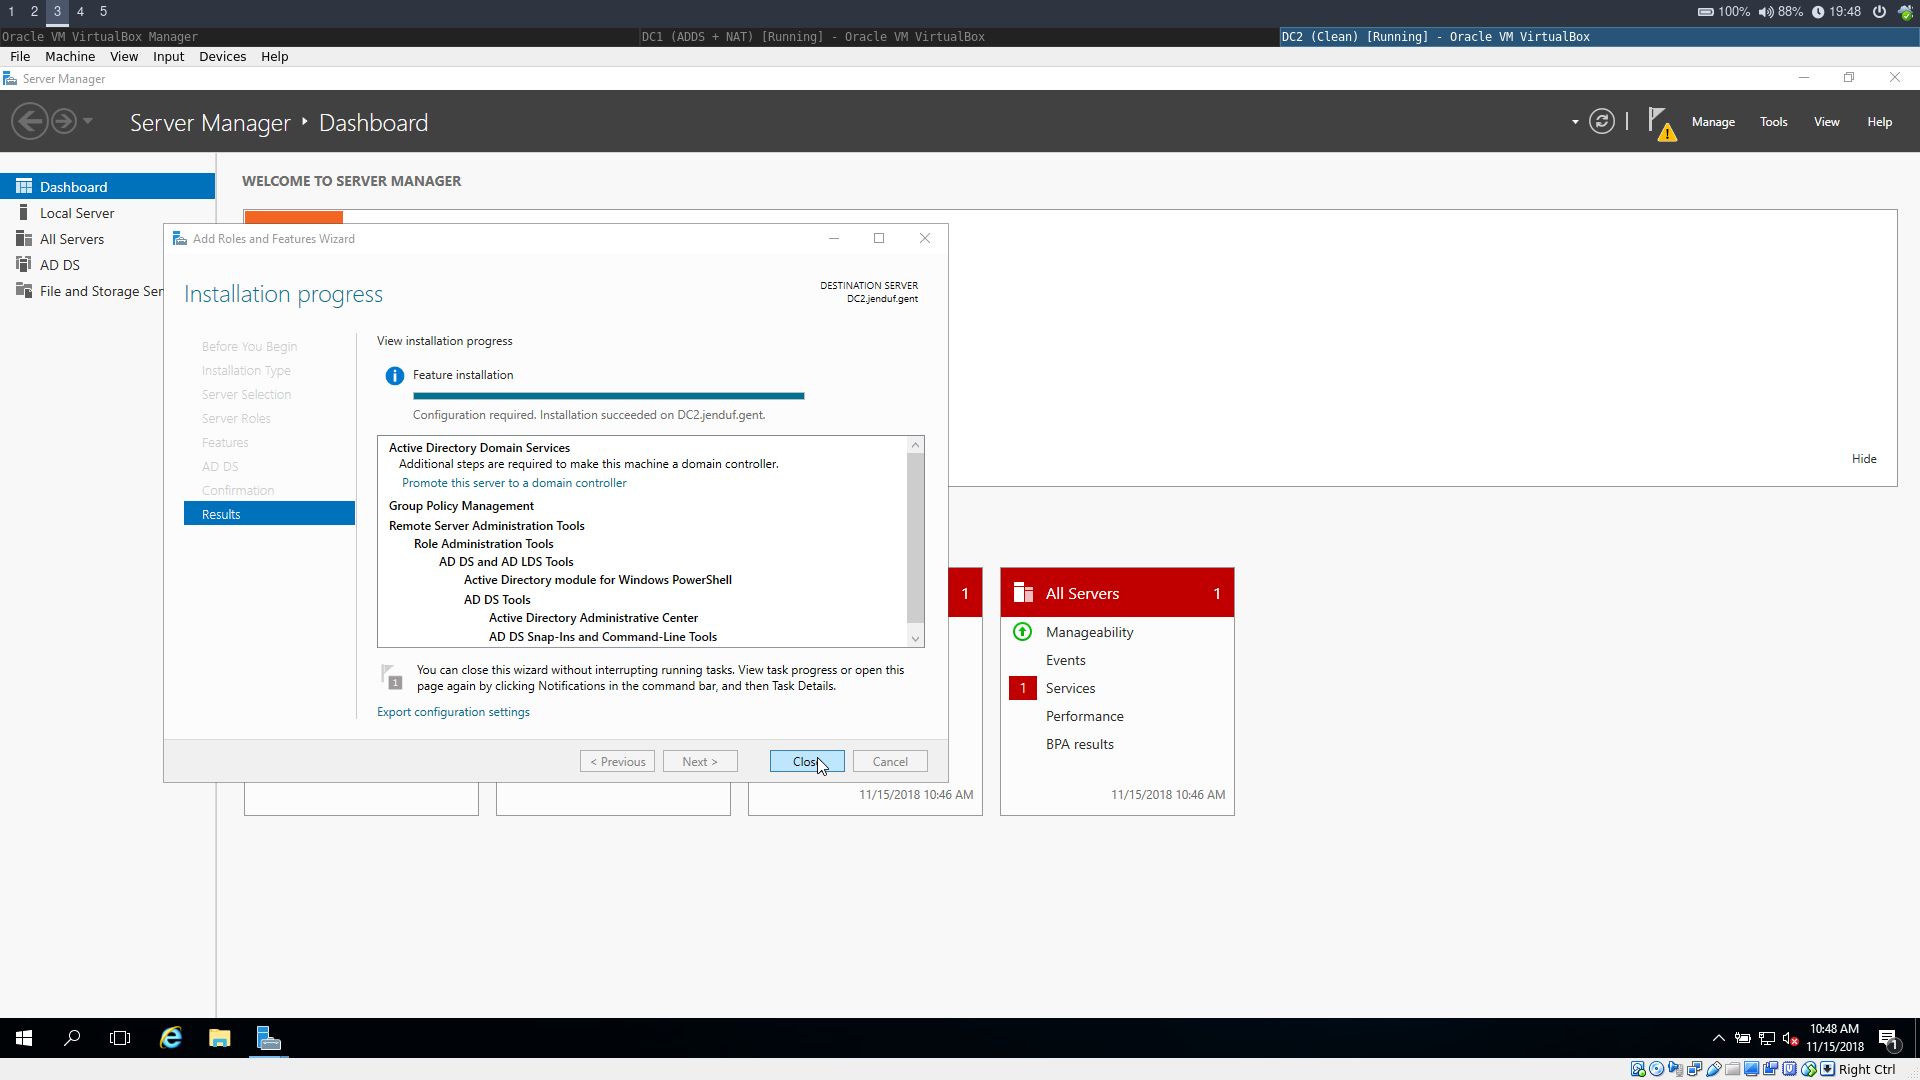
\includegraphics[width=15cm]{Pictures/DC2/ADDS/1542307695.png}
\end{center}
\begin{center}
	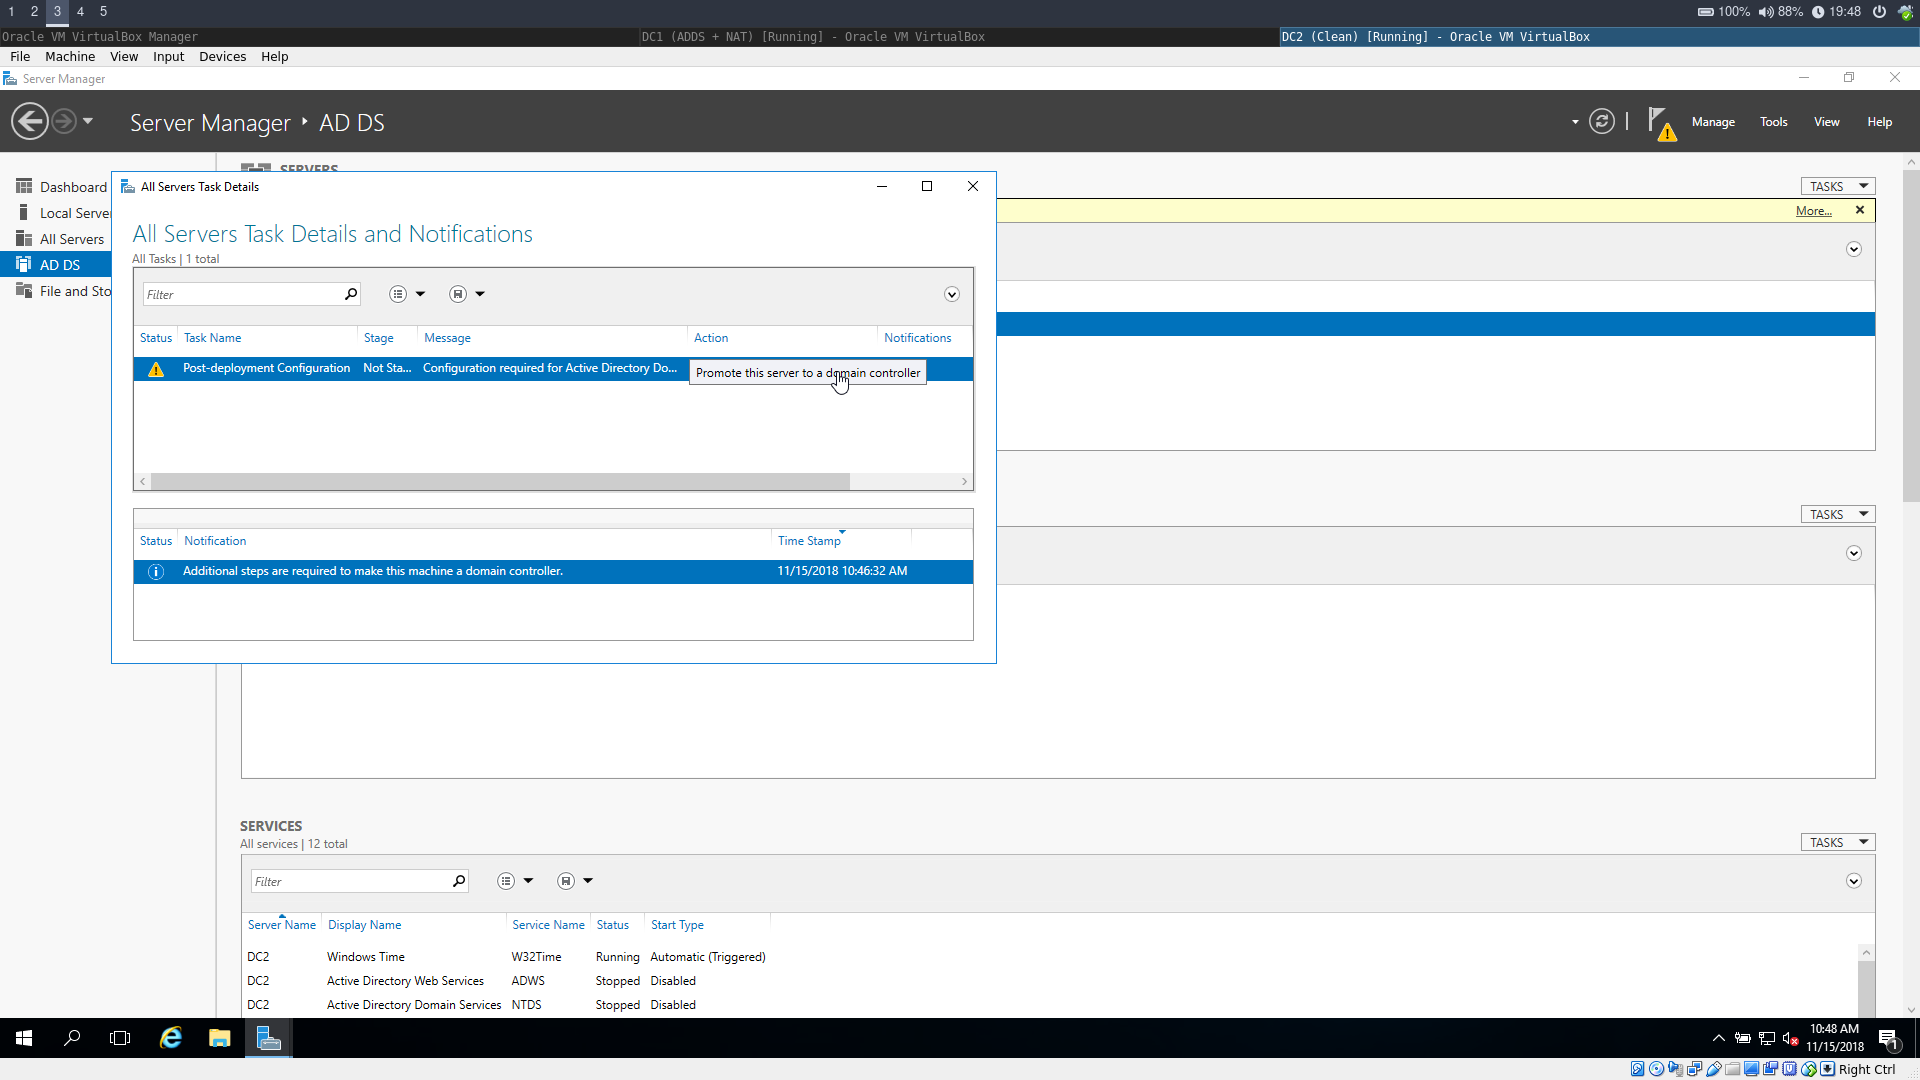
\includegraphics[width=15cm]{Pictures/DC2/ADDS/1542307706.png}
	
	Promoveer de server tot een domeincontroller.
\end{center}
\begin{center}
	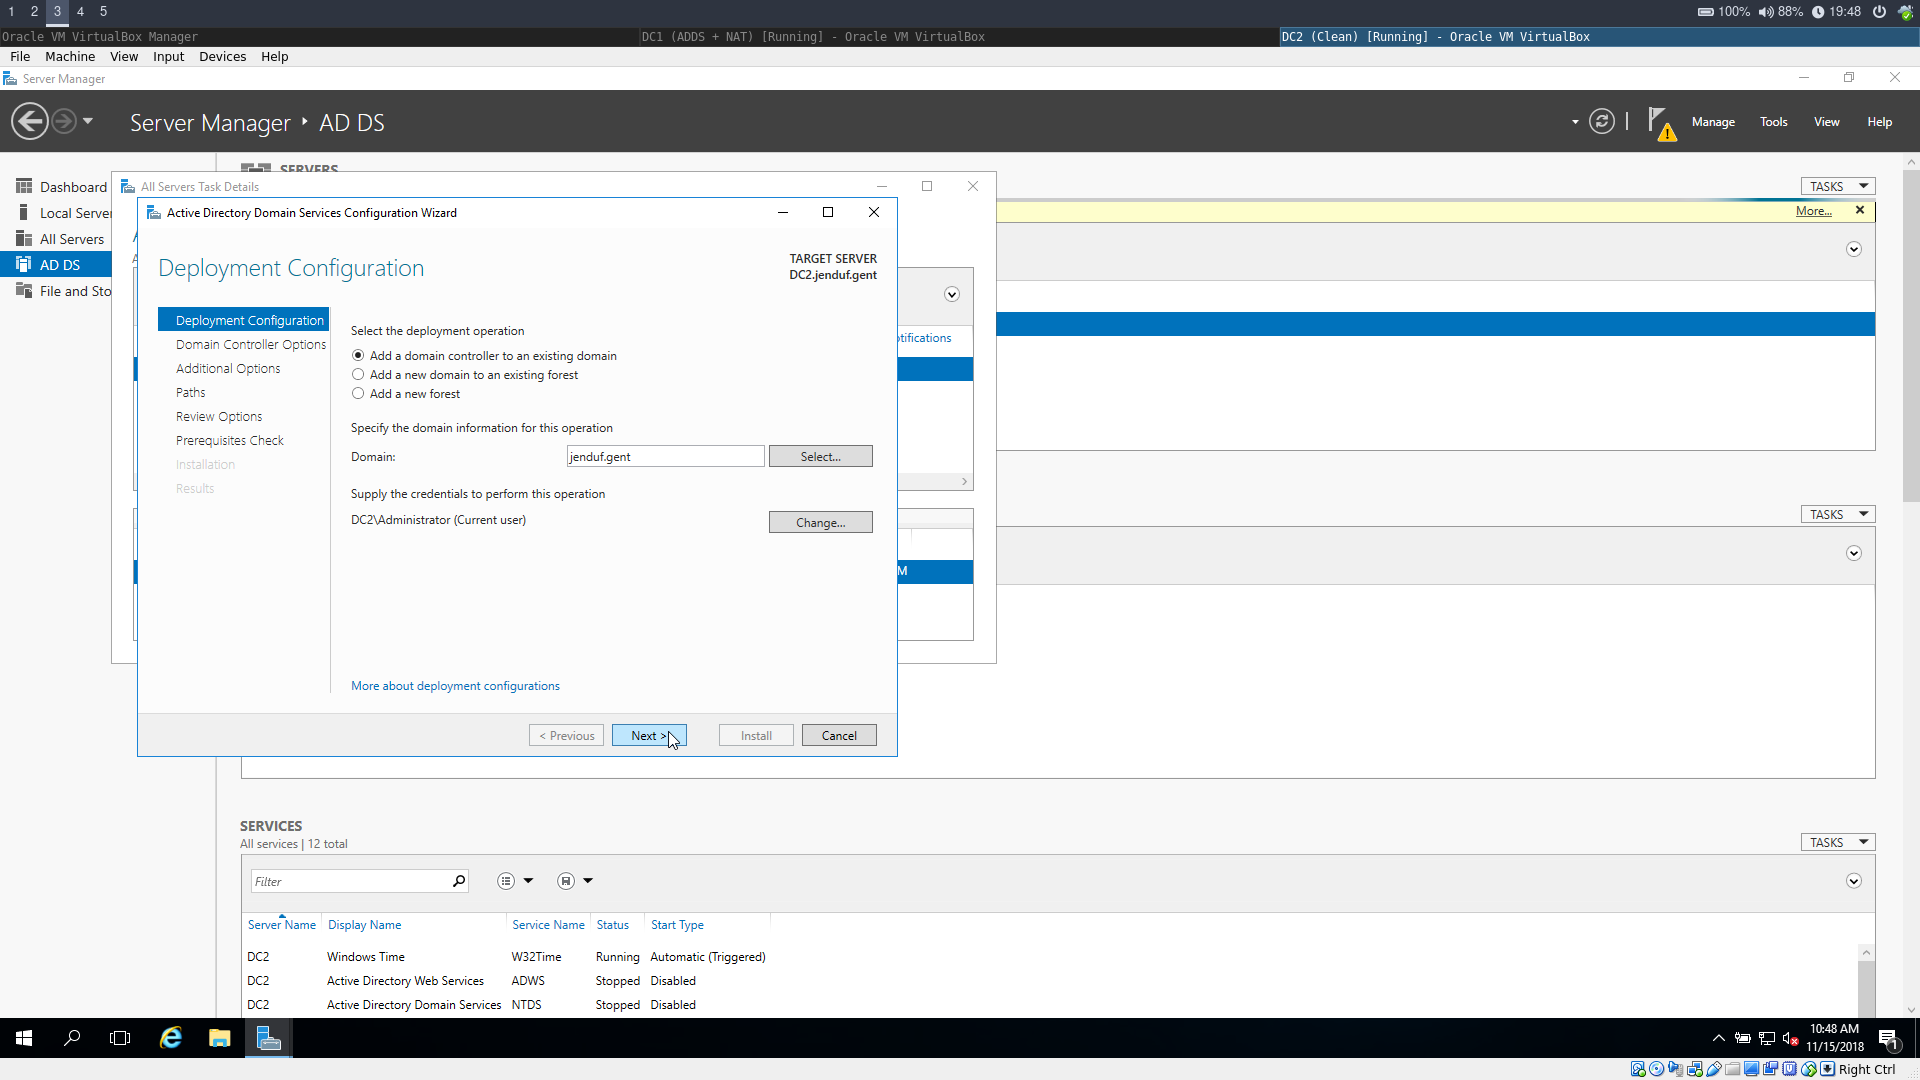
\includegraphics[width=15cm]{Pictures/DC2/ADDS/1542307727.png}
	
	Selecteer "Add domain controller to an existing domain".
\end{center}
\begin{center}
	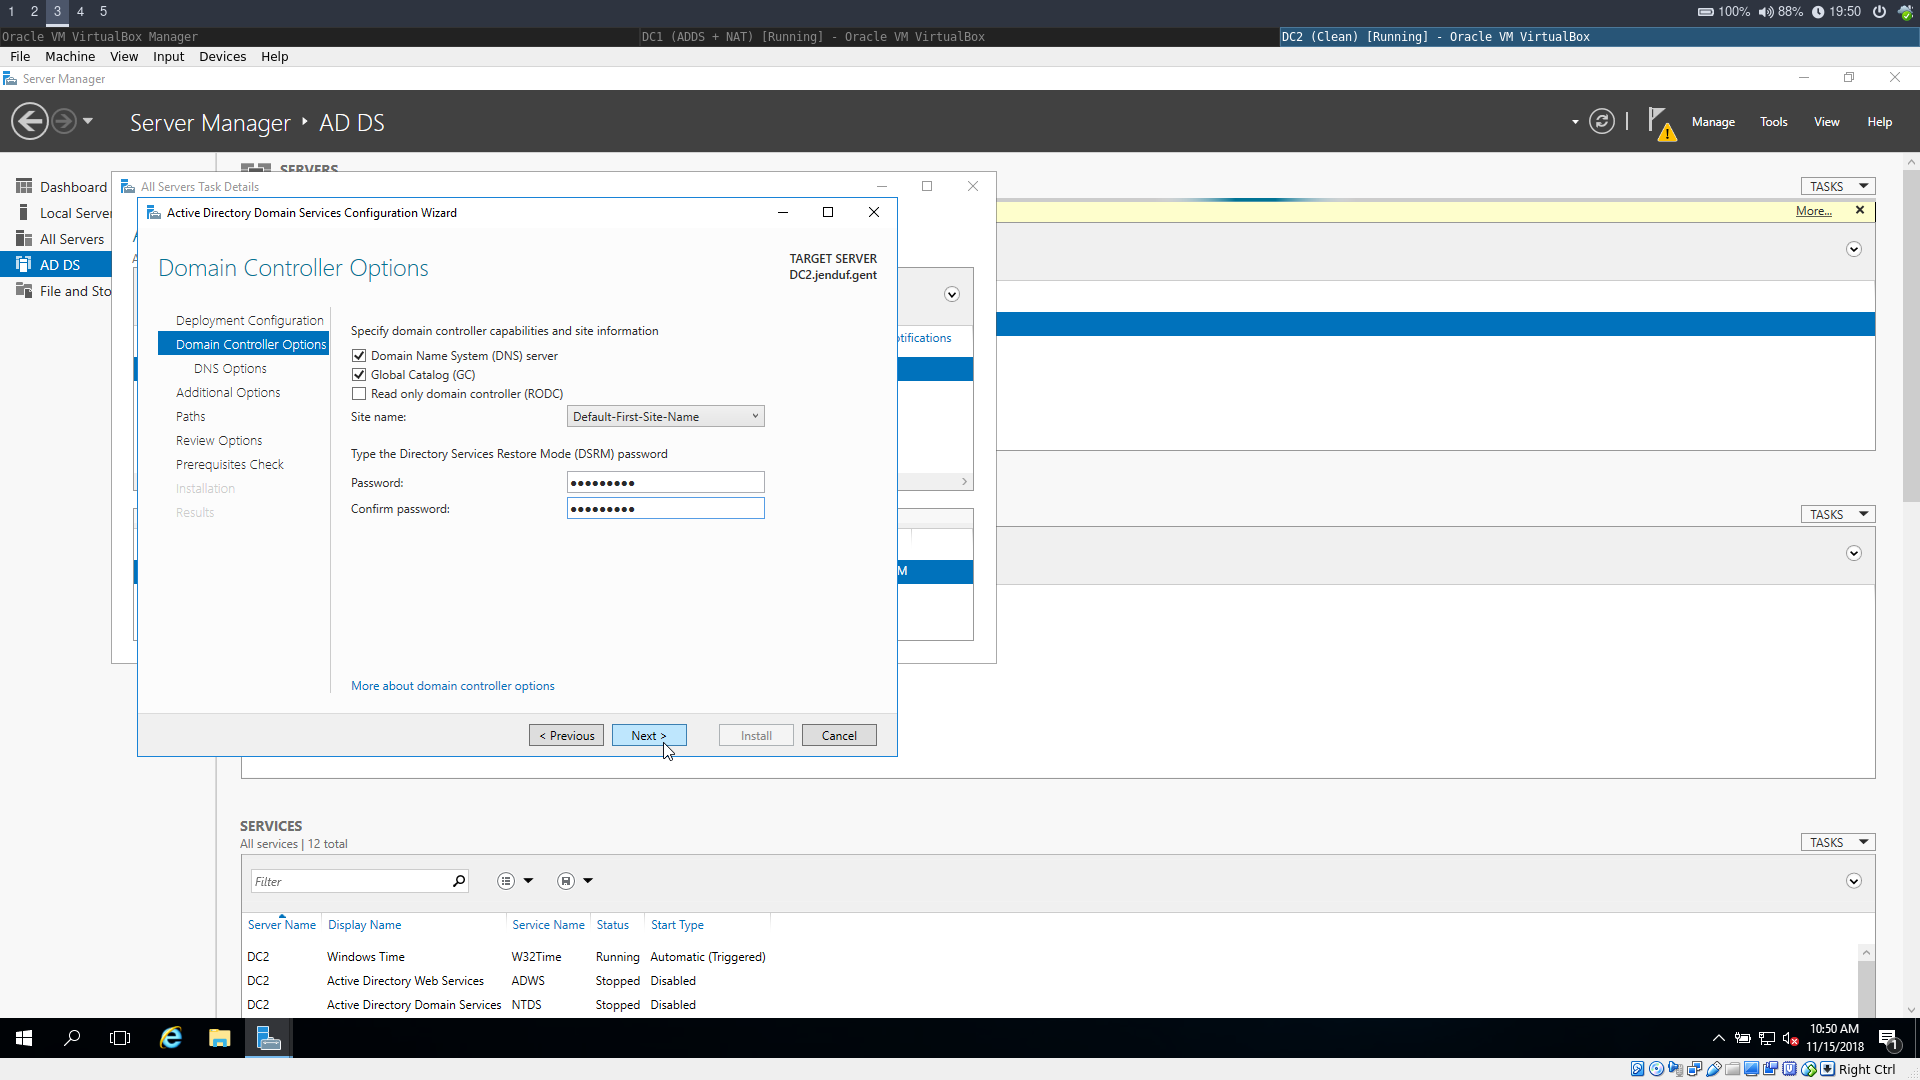
\includegraphics[width=15cm]{Pictures/DC2/ADDS/1542307813.png}
	
	Kies als paswoord opnieuw "Admin2018".
\end{center}
\begin{center}
	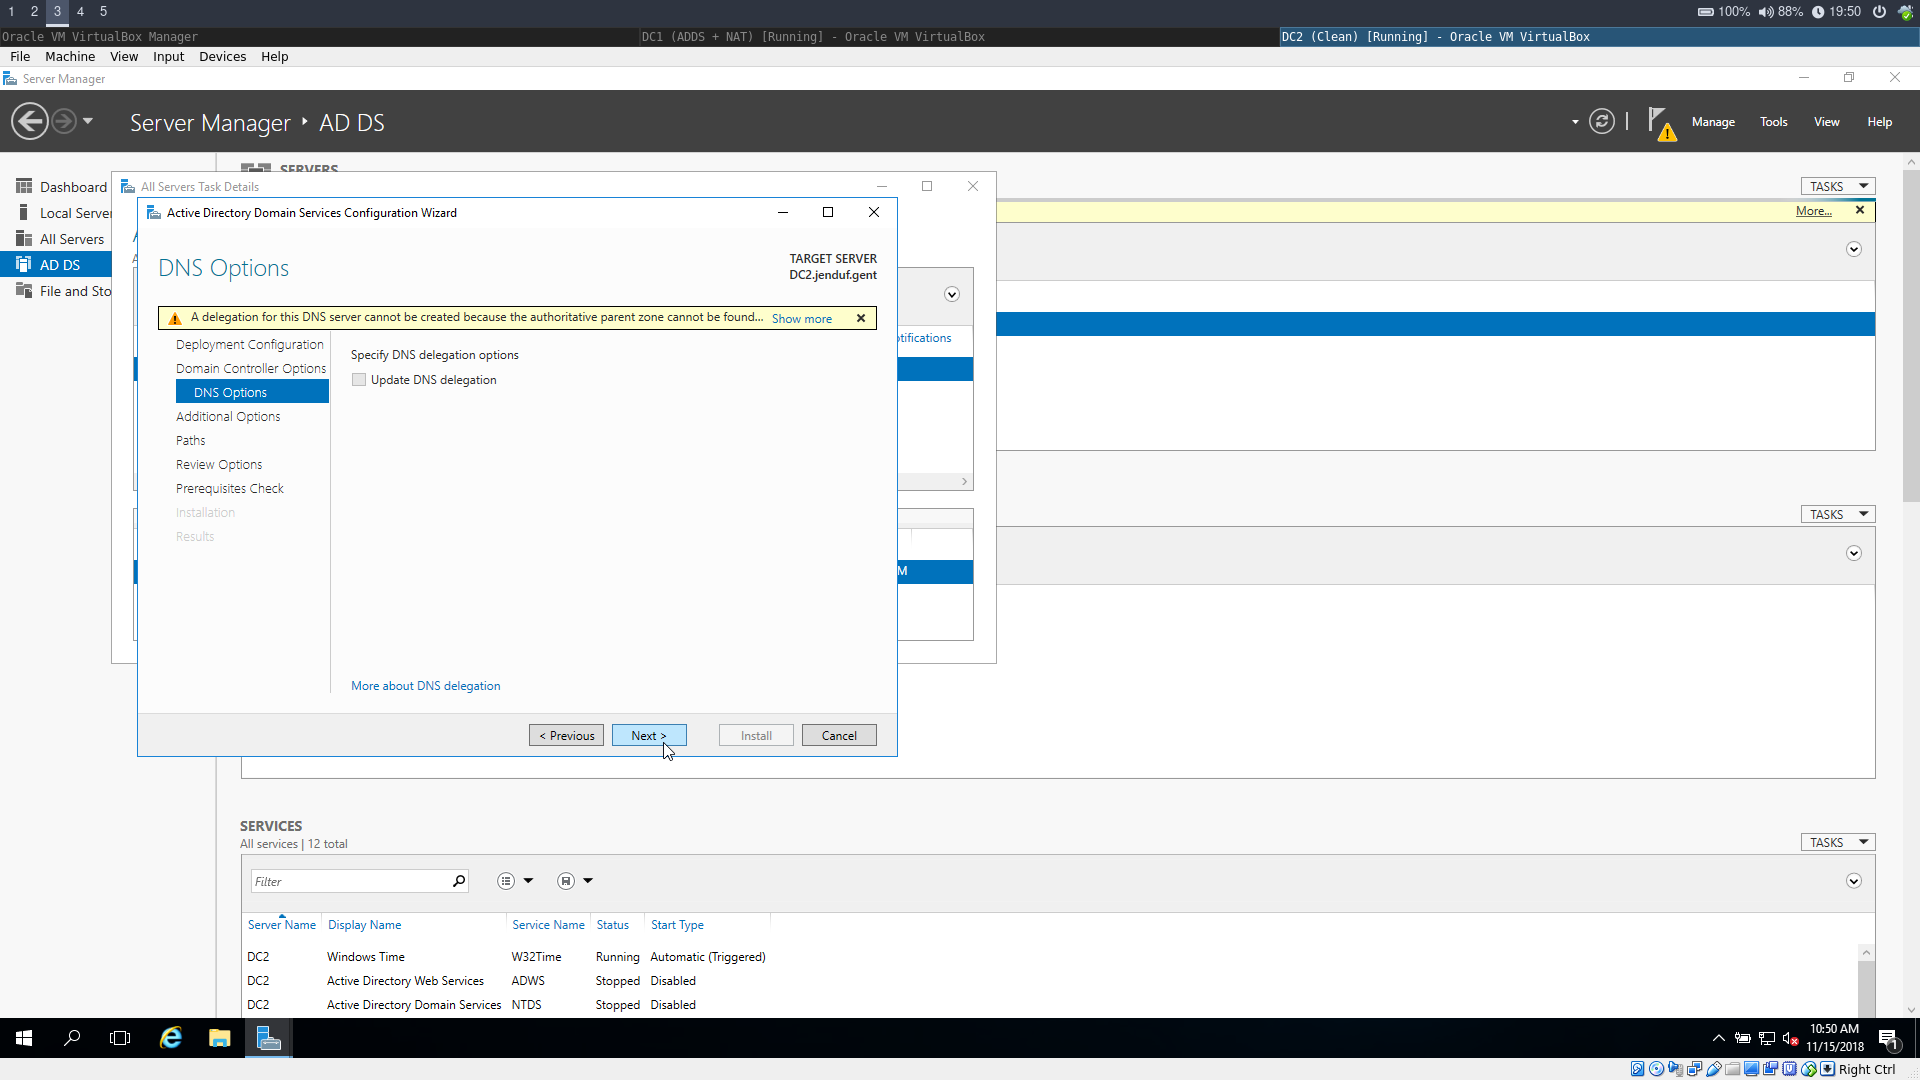
\includegraphics[width=15cm]{Pictures/DC2/ADDS/1542307817.png}
	
	Volg de configuratiewizard verder.
\end{center}
\begin{center}
	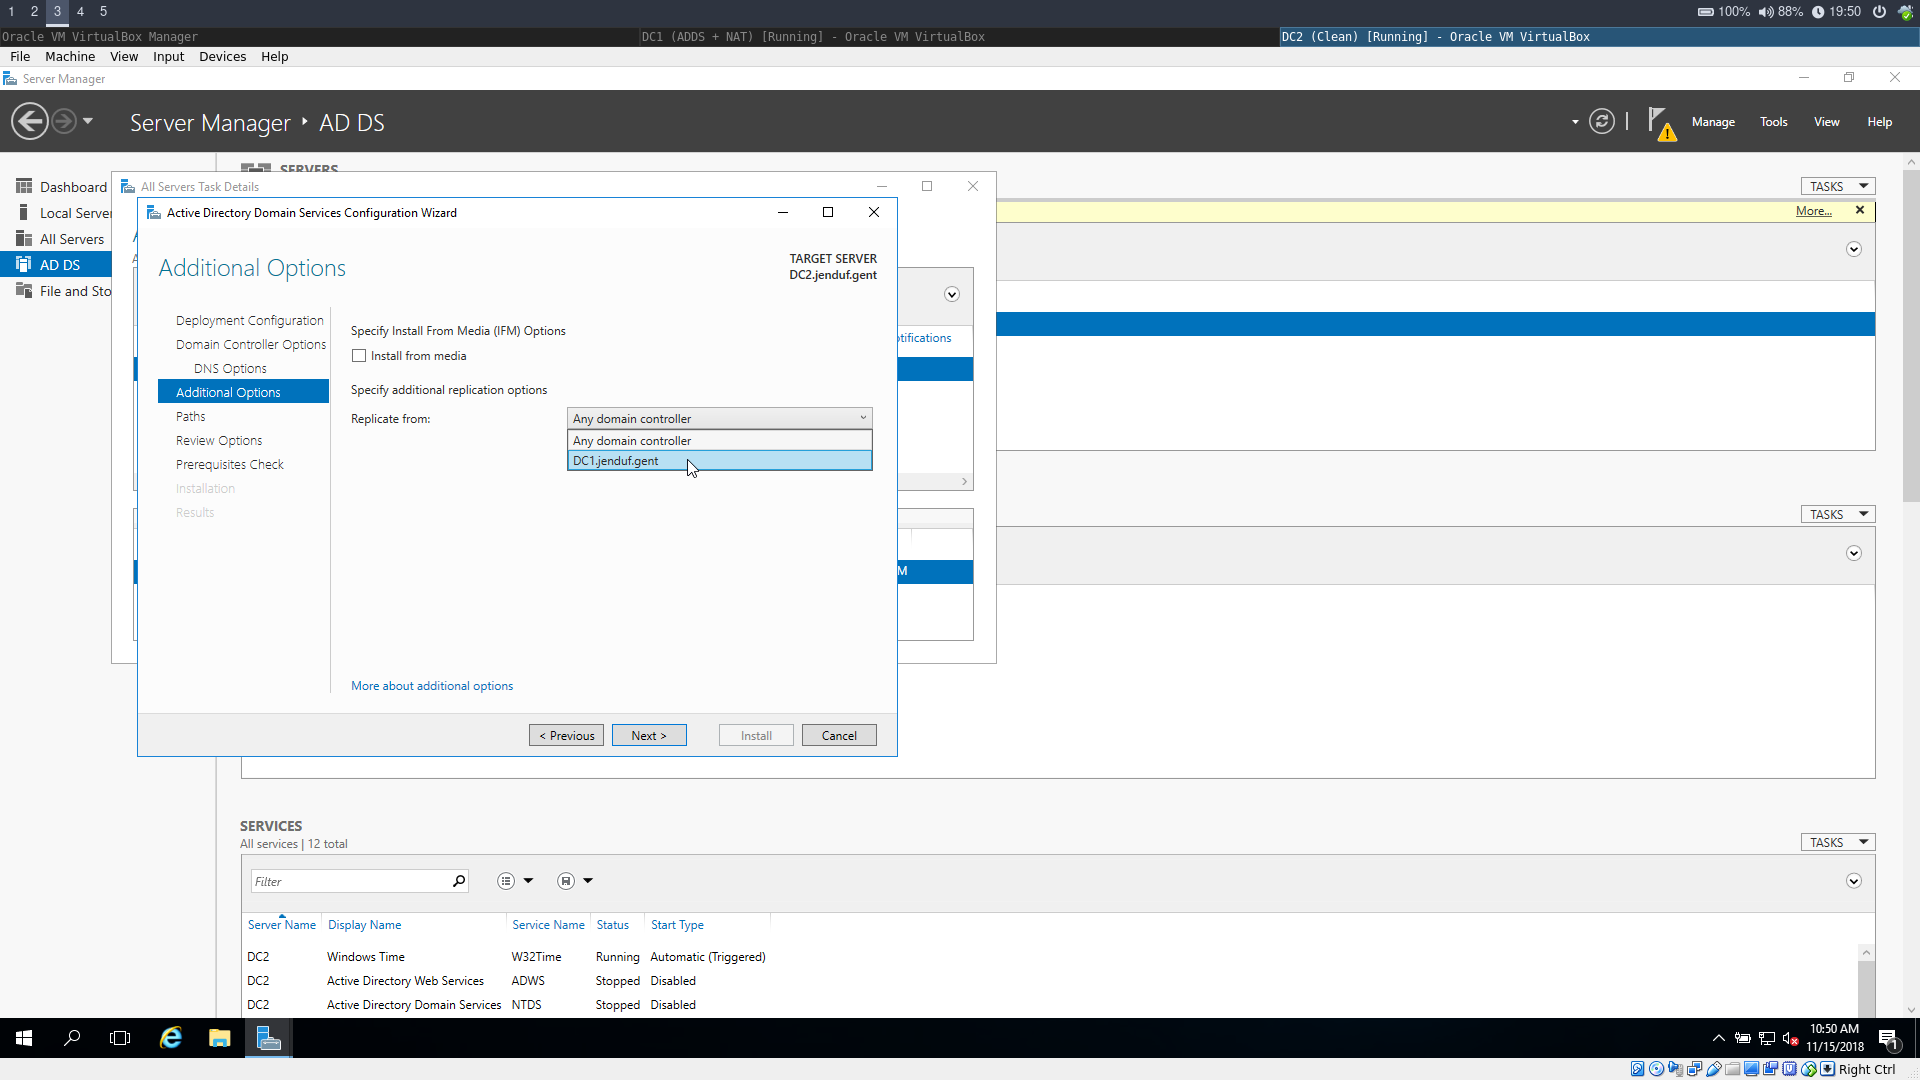
\includegraphics[width=15cm]{Pictures/DC2/ADDS/1542307822.png}
	
	Replicate van "DC1.jenduf.gent"
\end{center}
\begin{center}
	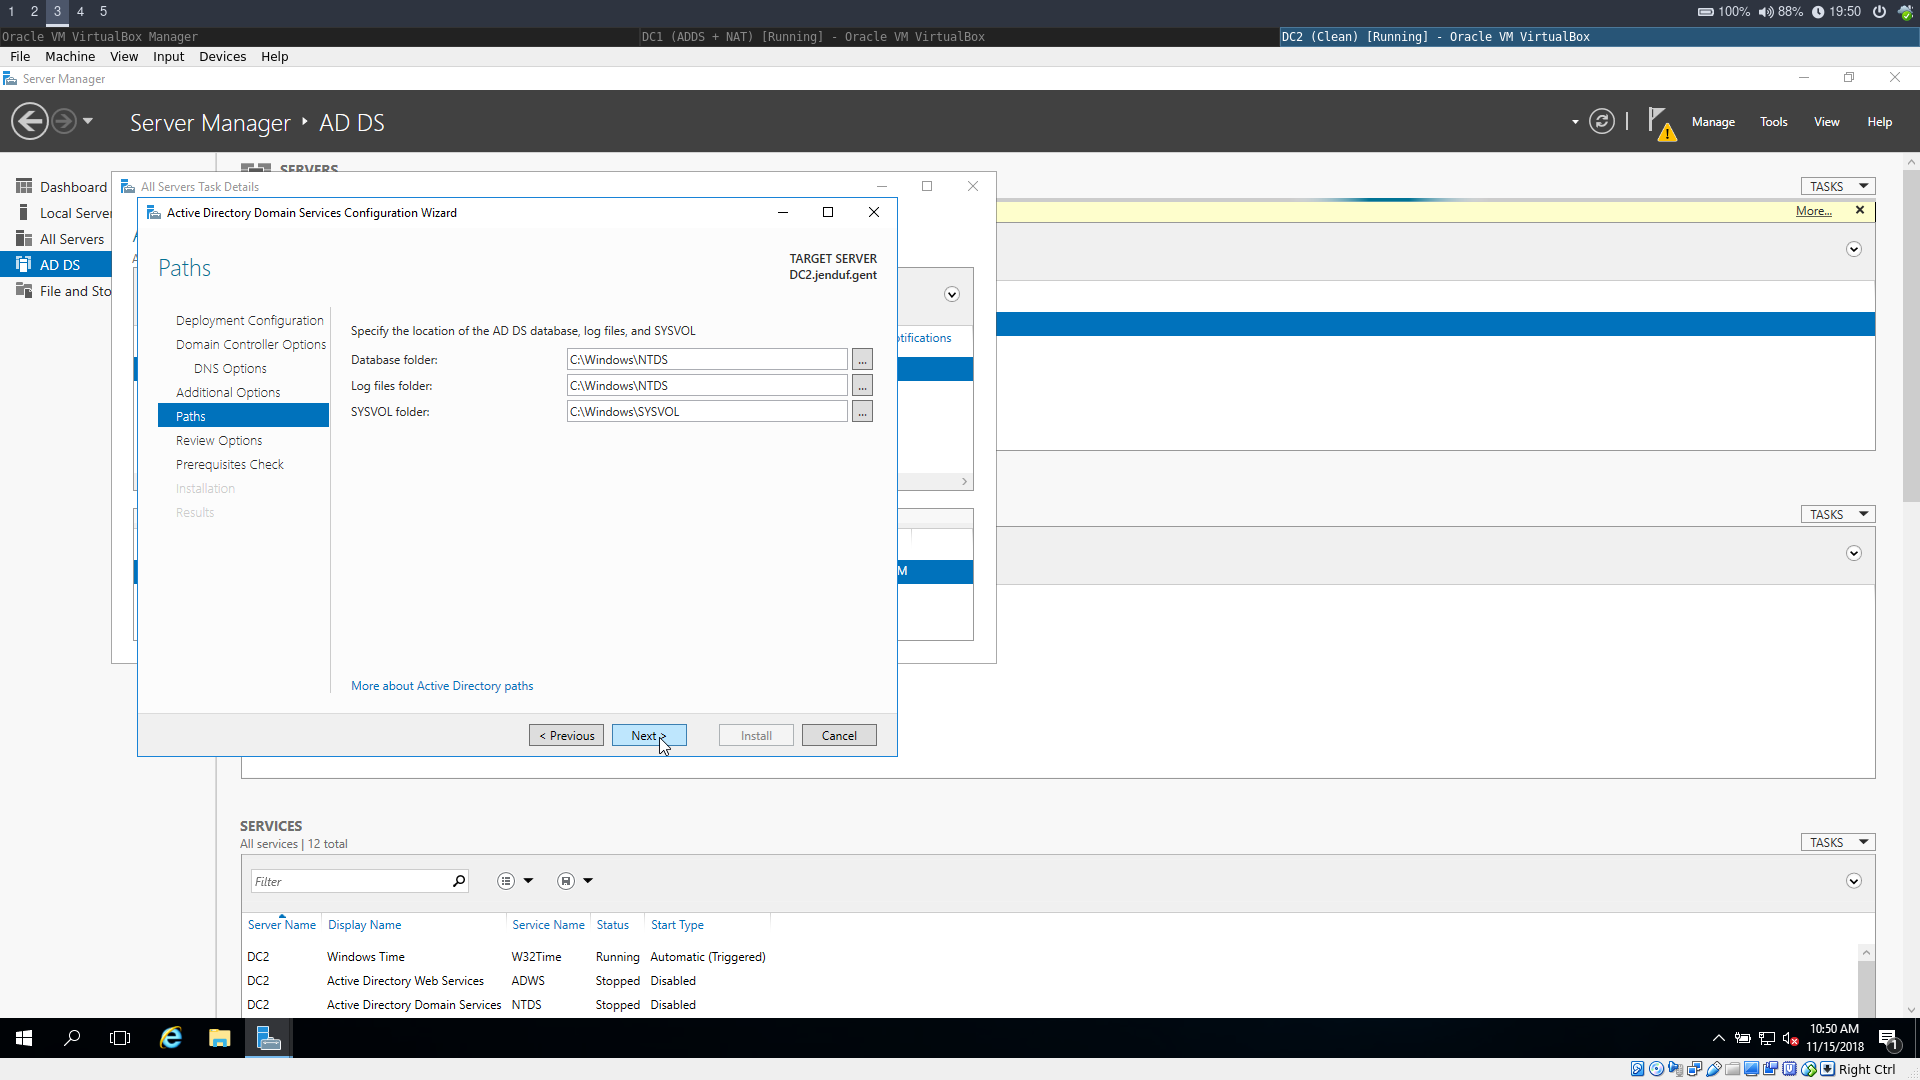
\includegraphics[width=15cm]{Pictures/DC2/ADDS/1542307825.png}
\end{center}
\begin{center}
	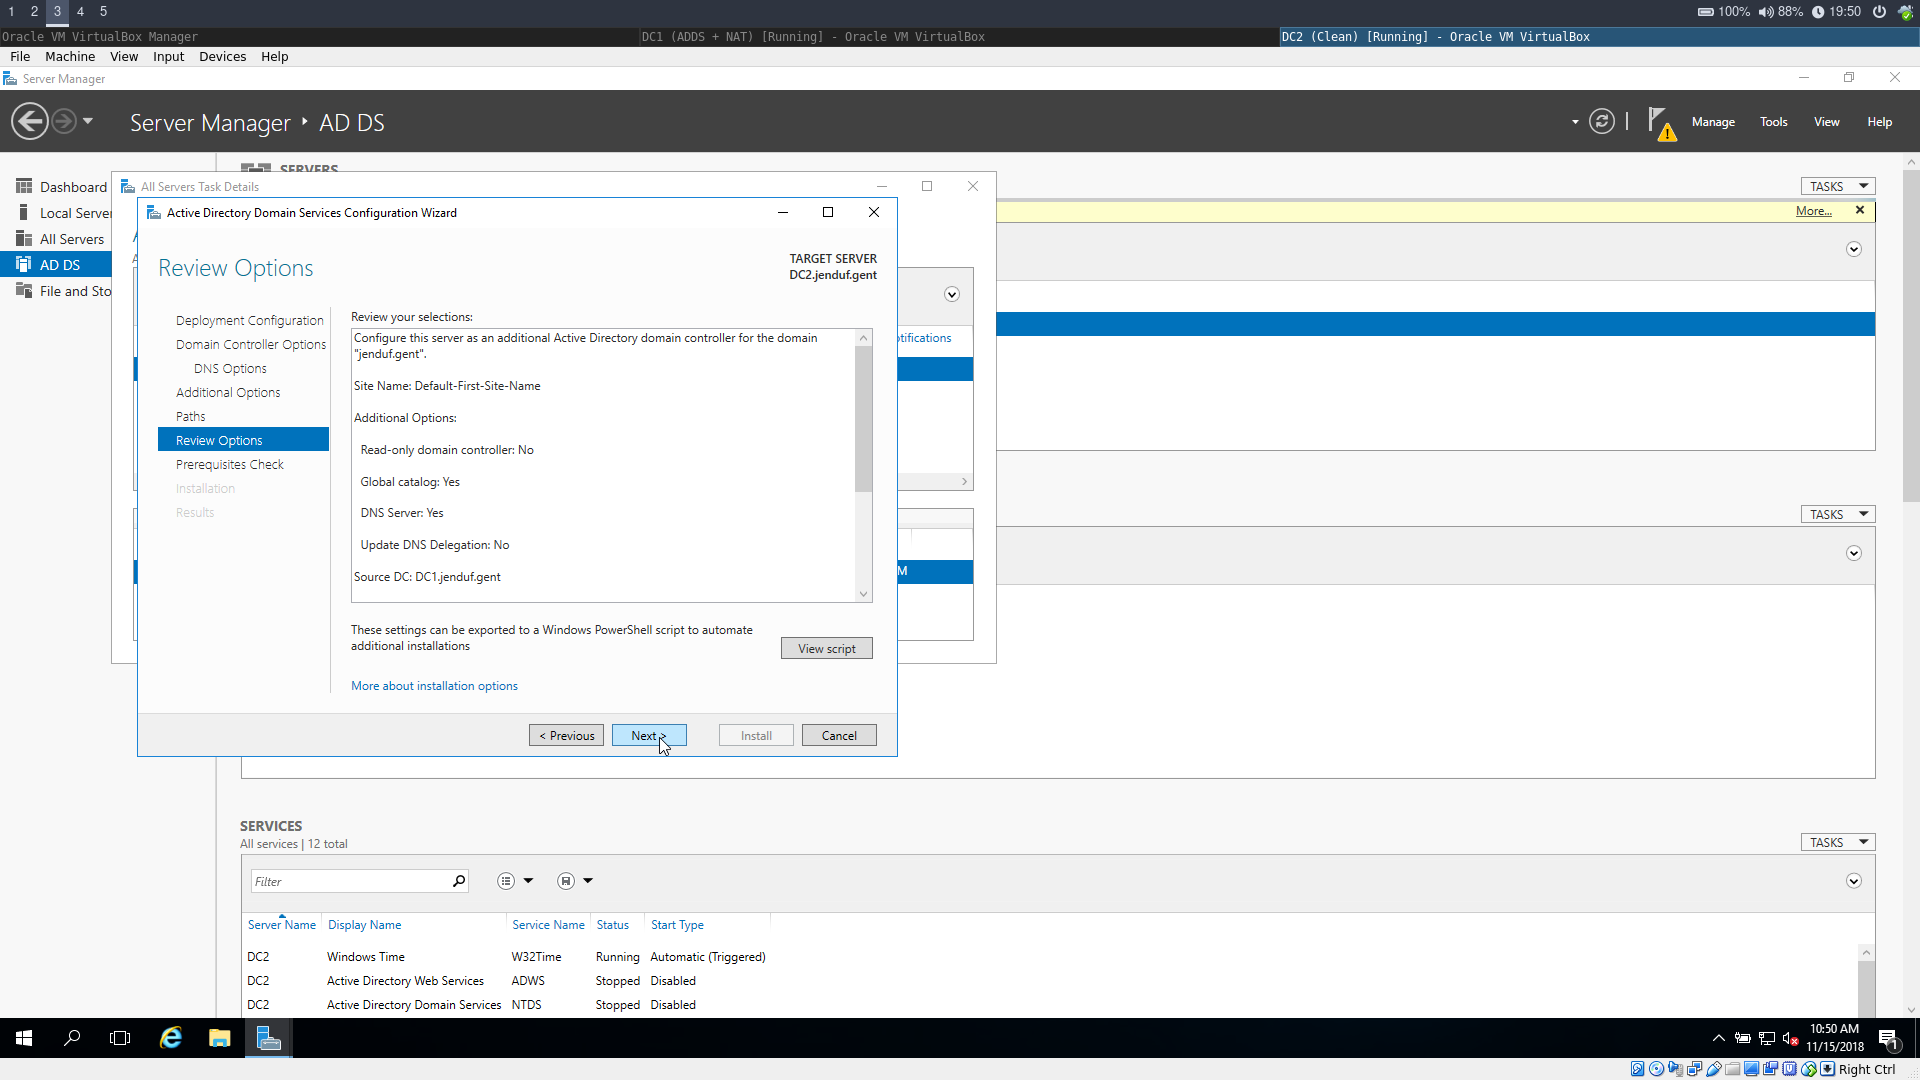
\includegraphics[width=15cm]{Pictures/DC2/ADDS/1542307828.png}
\end{center}
\begin{center}
	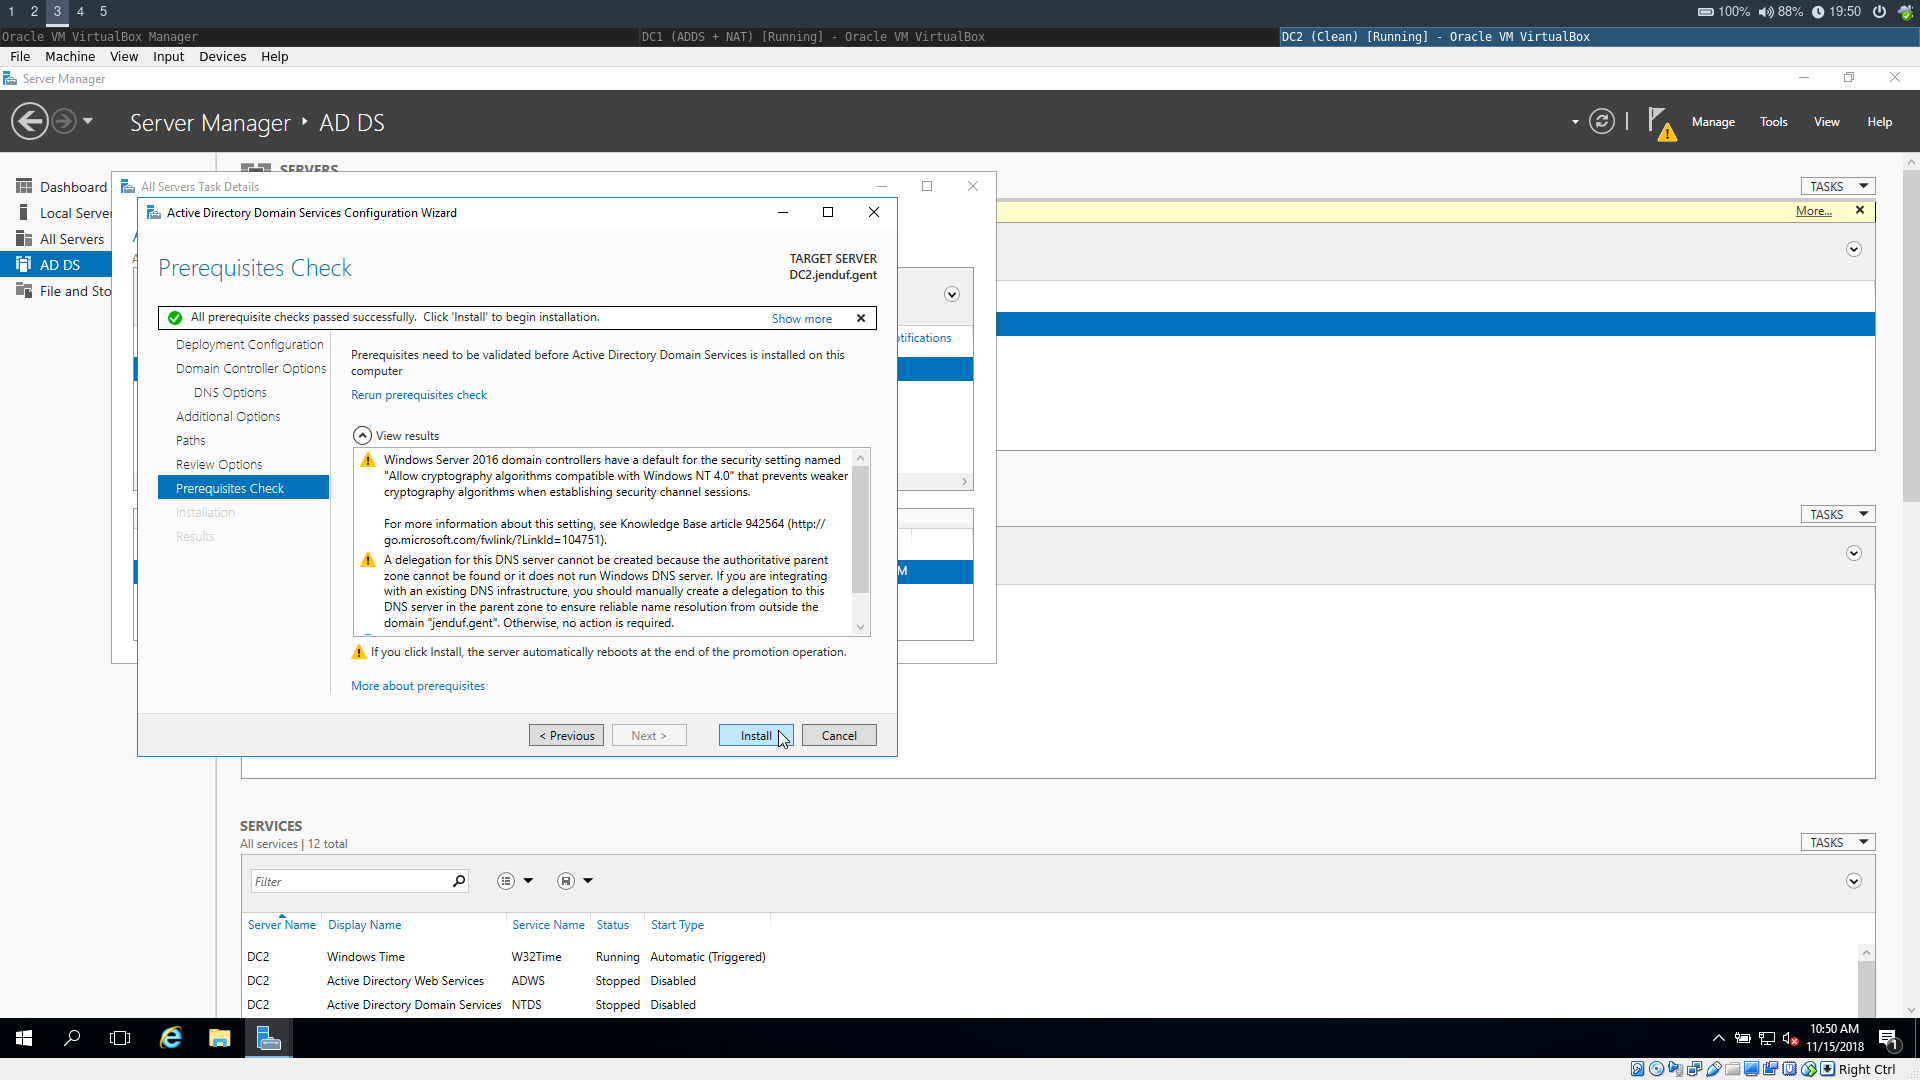
\includegraphics[width=15cm]{Pictures/DC2/ADDS/1542307834.png}
\end{center}
\begin{center}
	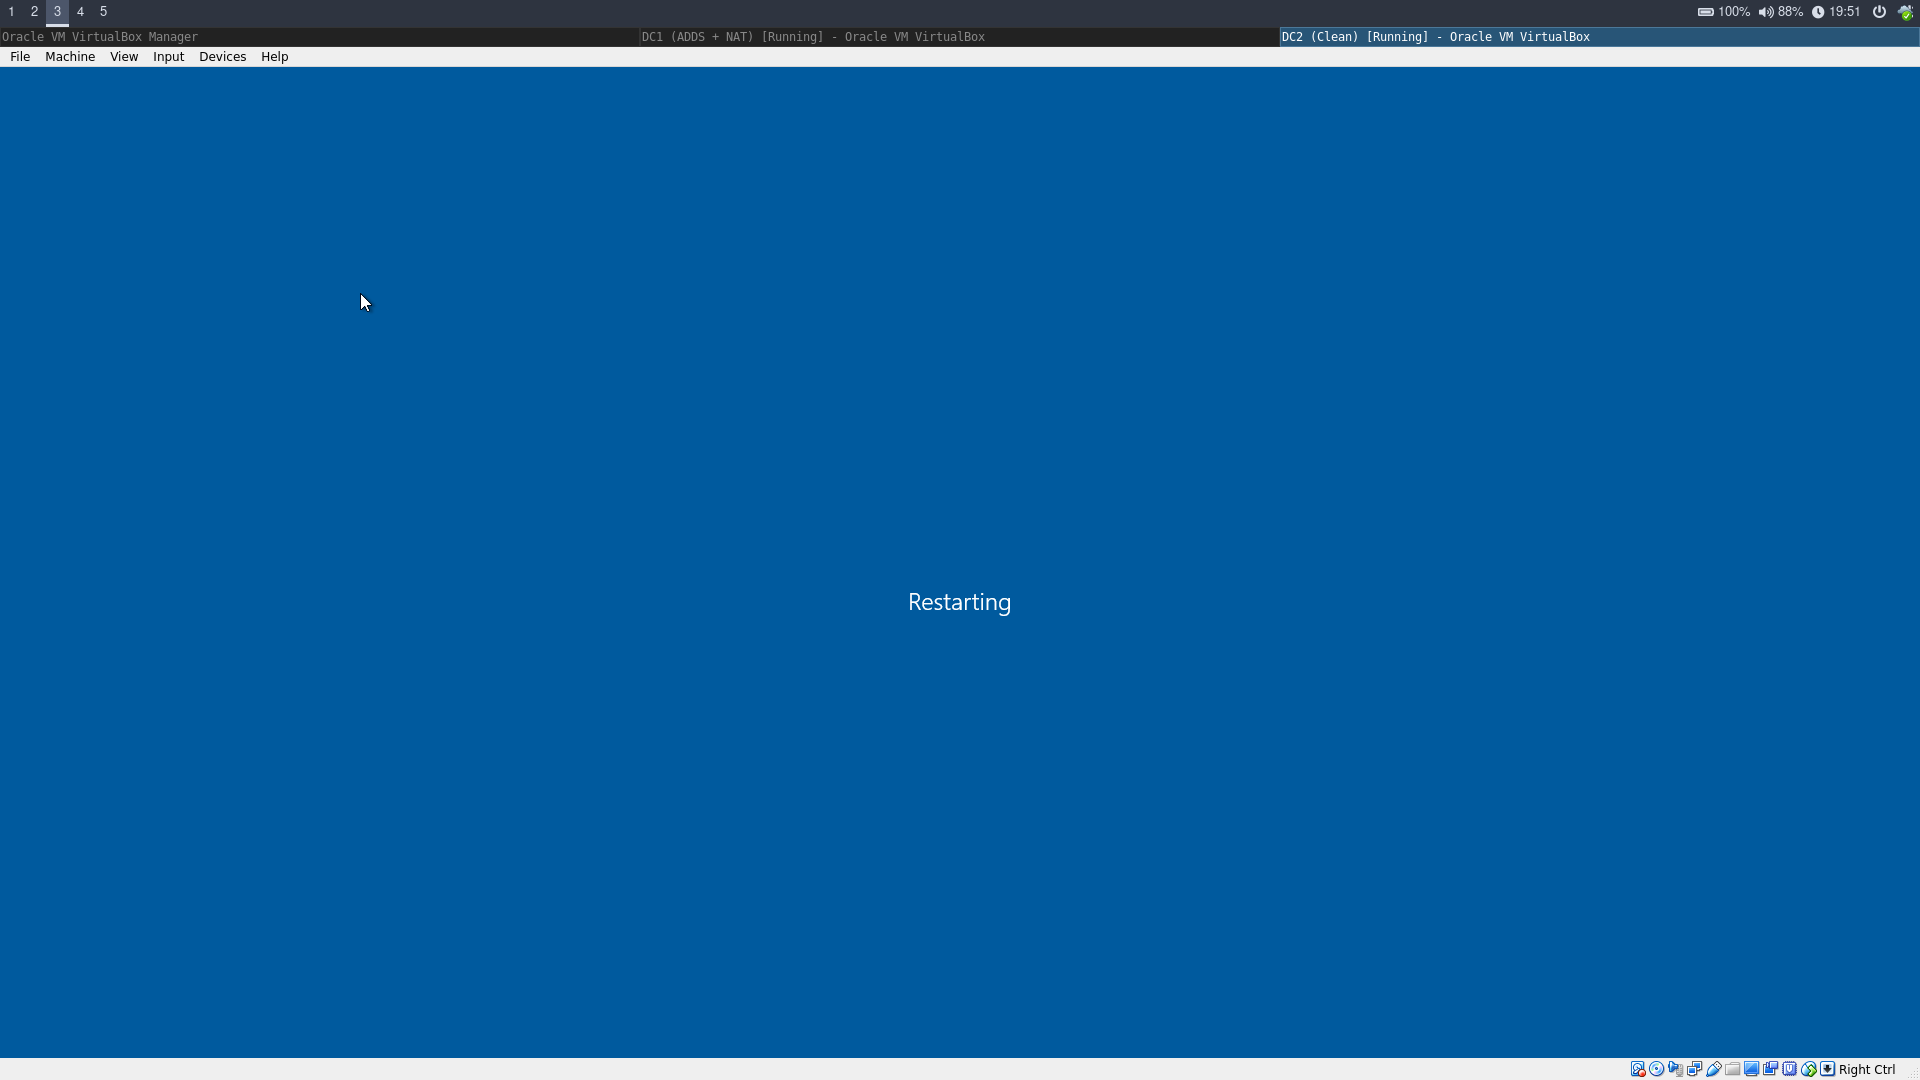
\includegraphics[width=15cm]{Pictures/DC2/ADDS/1542307904.png}
\end{center}

\section{Configuratie DHCP}

\begin{center}
	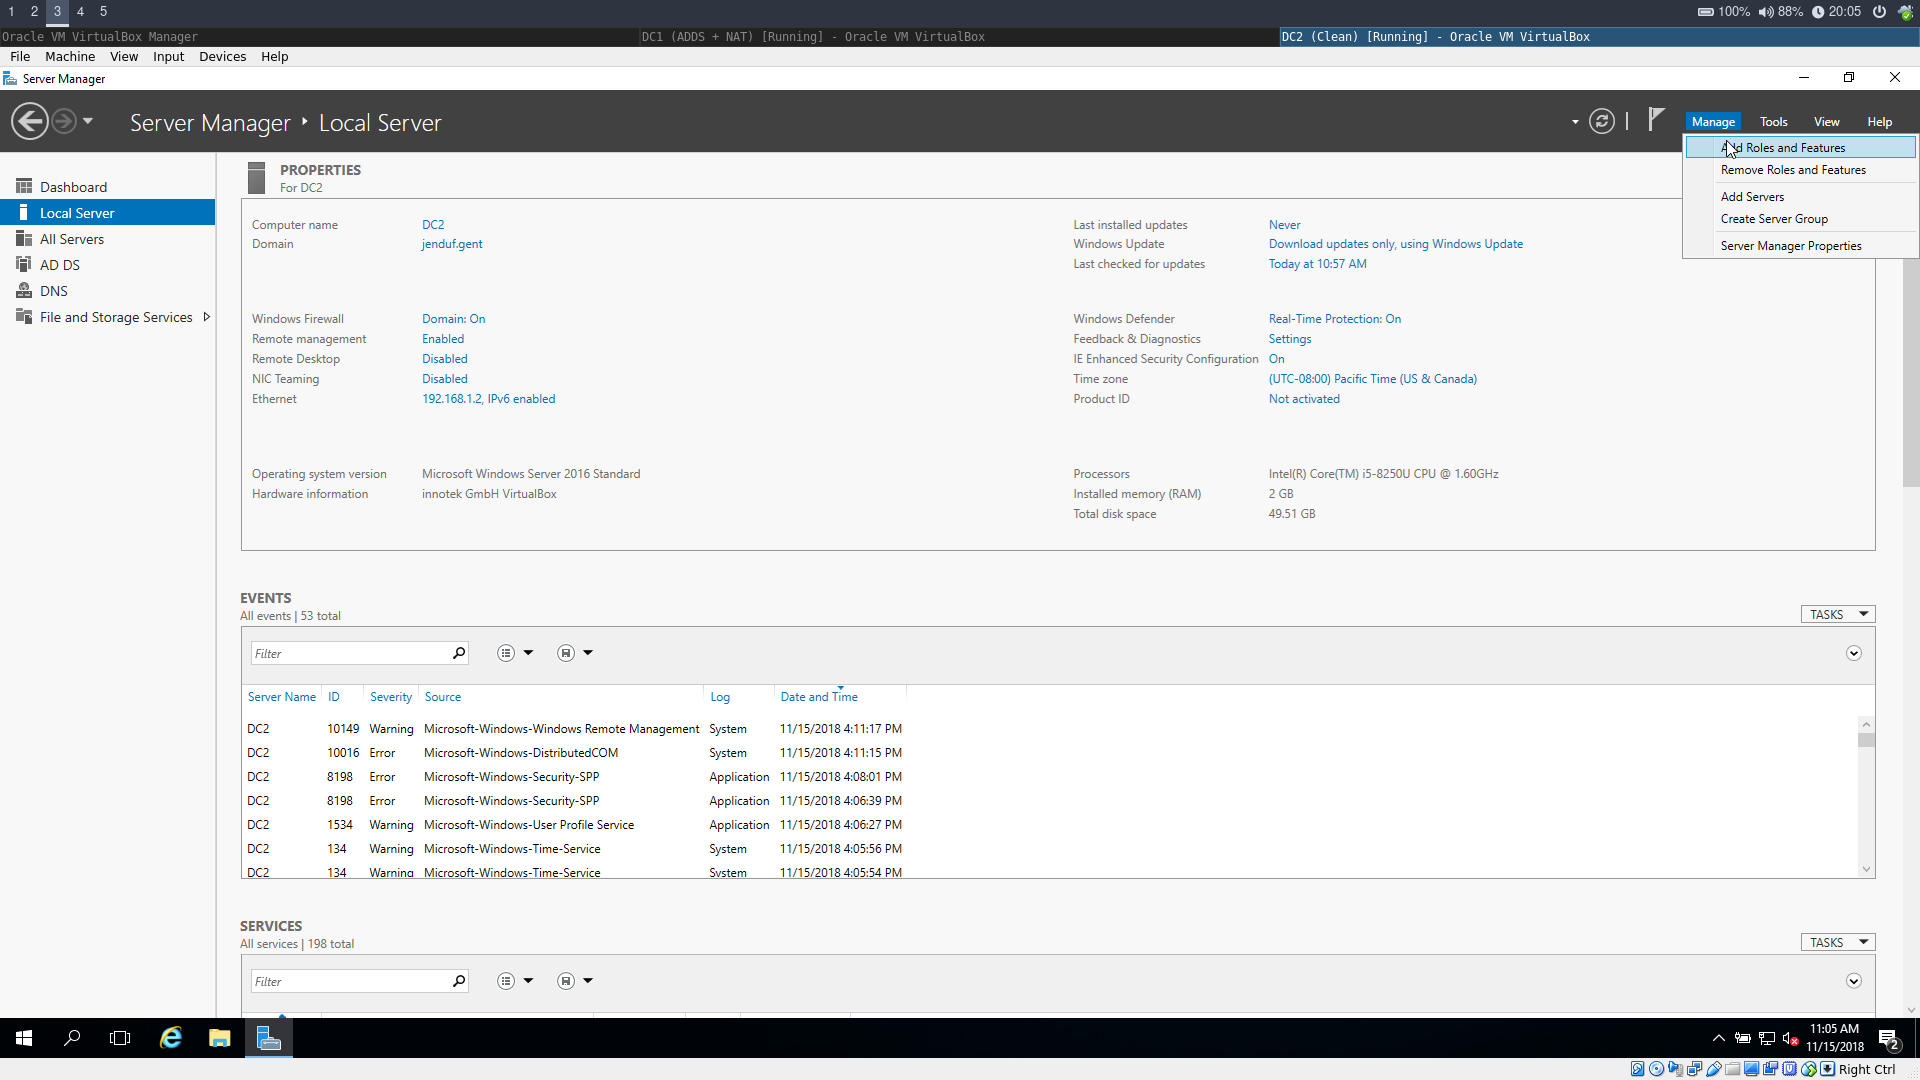
\includegraphics[width=15cm]{Pictures/DC2/DHCP/1542308705.png}
	
	Voeg een nieuwe rol toe aan de server.
\end{center}
\begin{center}
	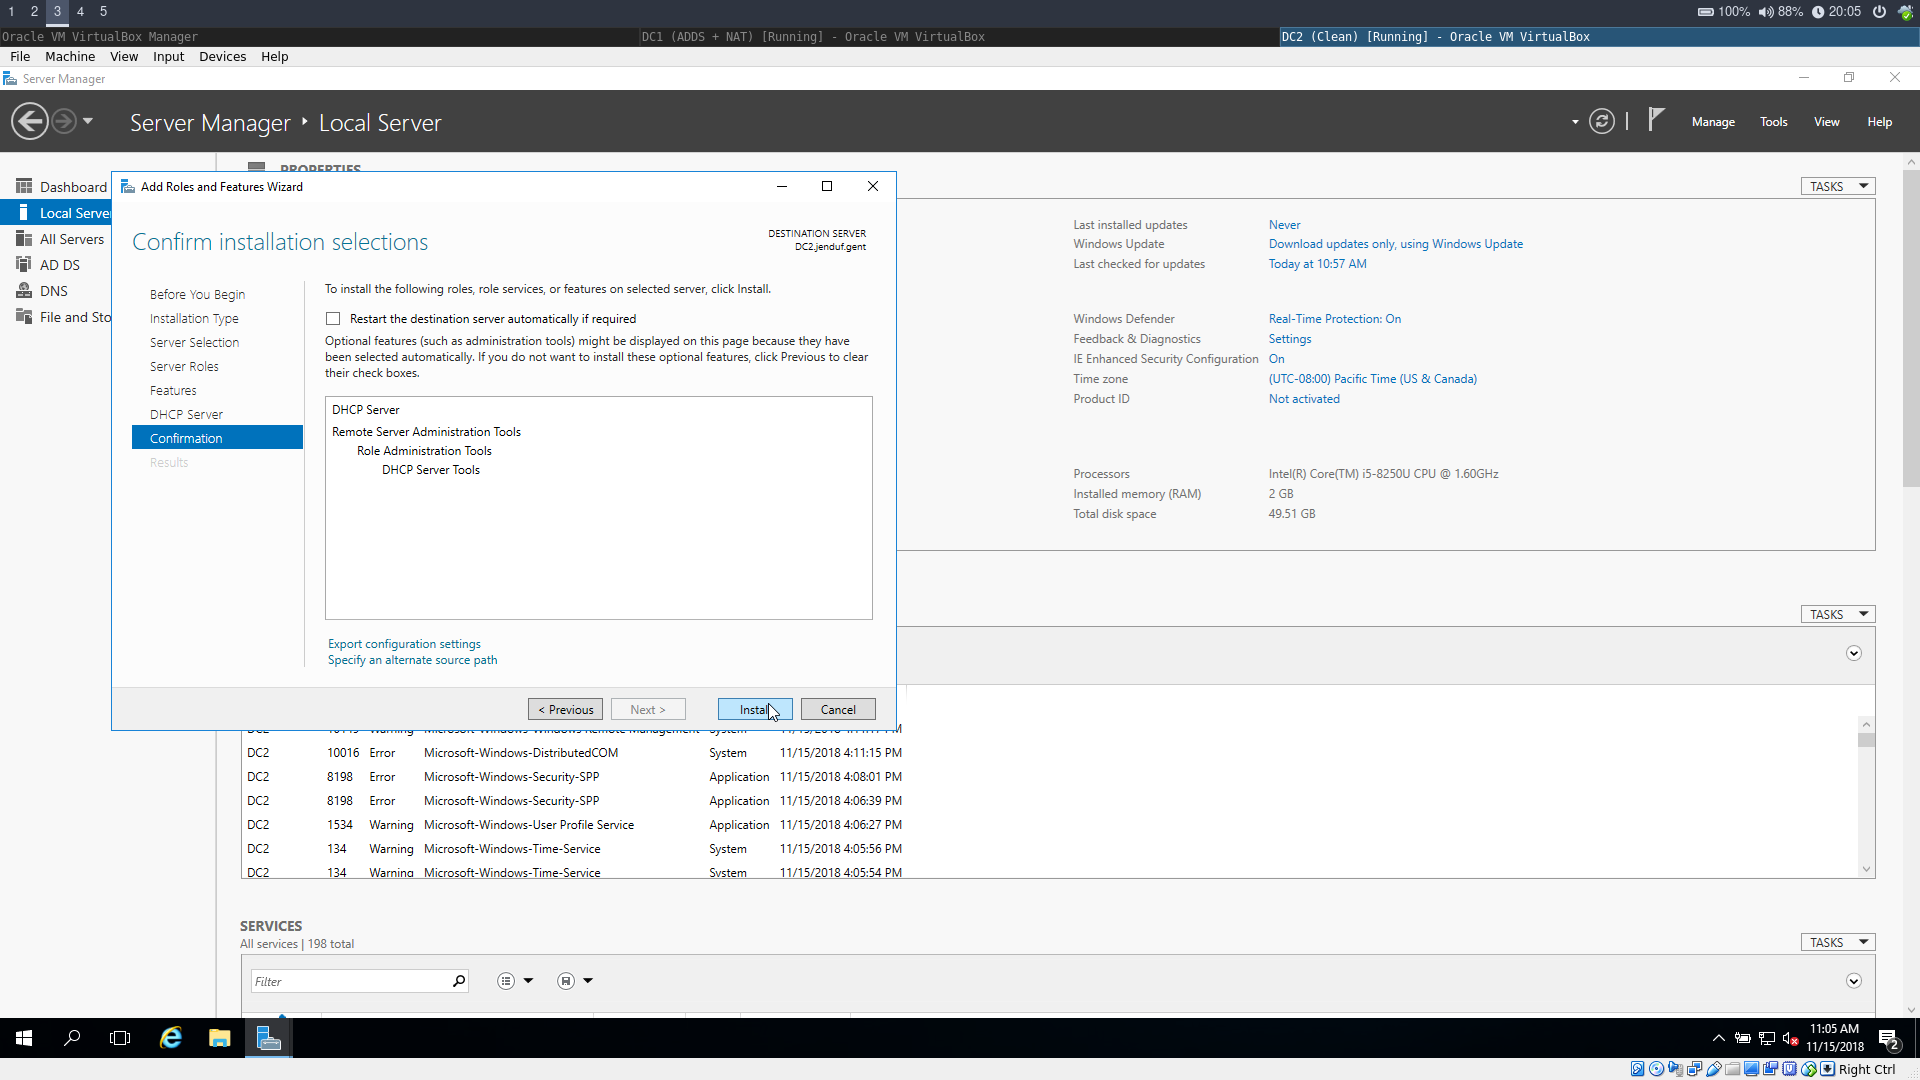
\includegraphics[width=15cm]{Pictures/DC2/DHCP/1542308722.png}
	
	Kies voor de DHCP Server.
\end{center}
\begin{center}
	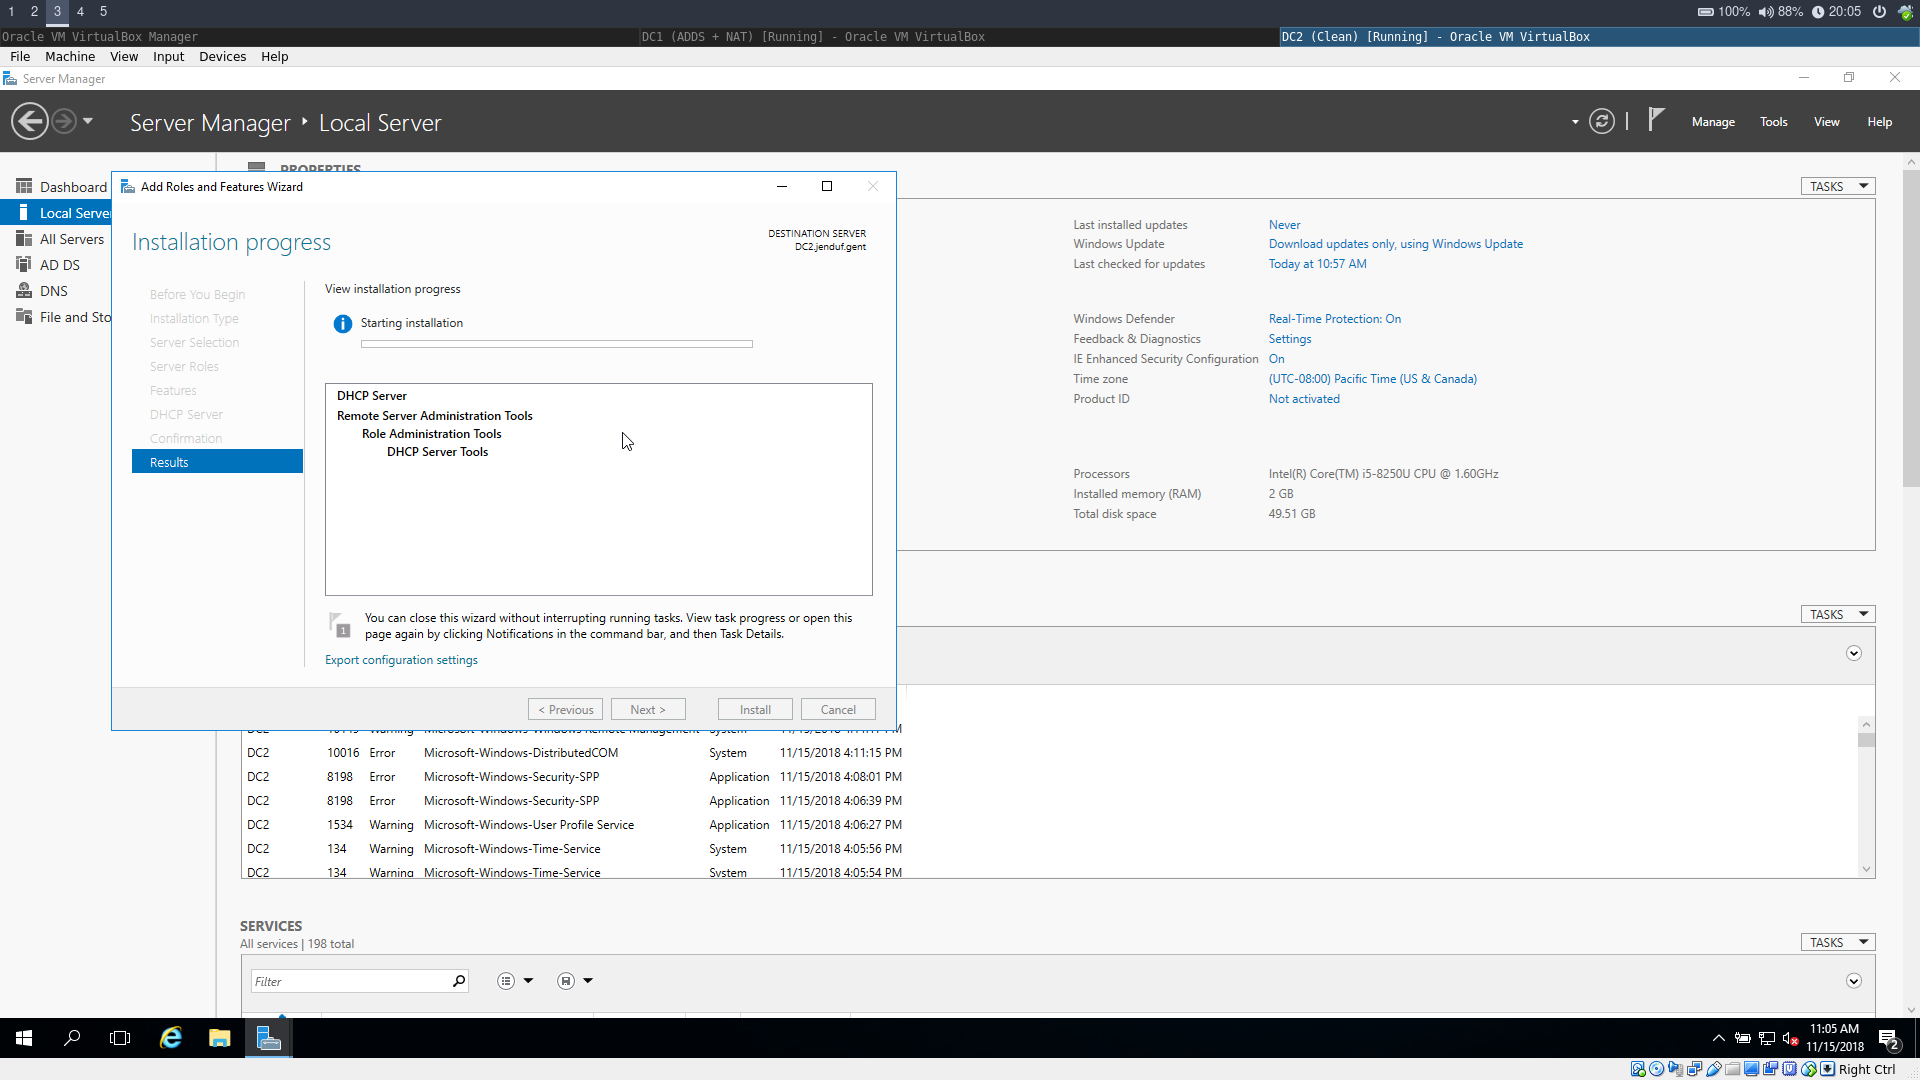
\includegraphics[width=15cm]{Pictures/DC2/DHCP/1542308725.png}
	
	Volg de installatiewizard.
\end{center}
\begin{center}
	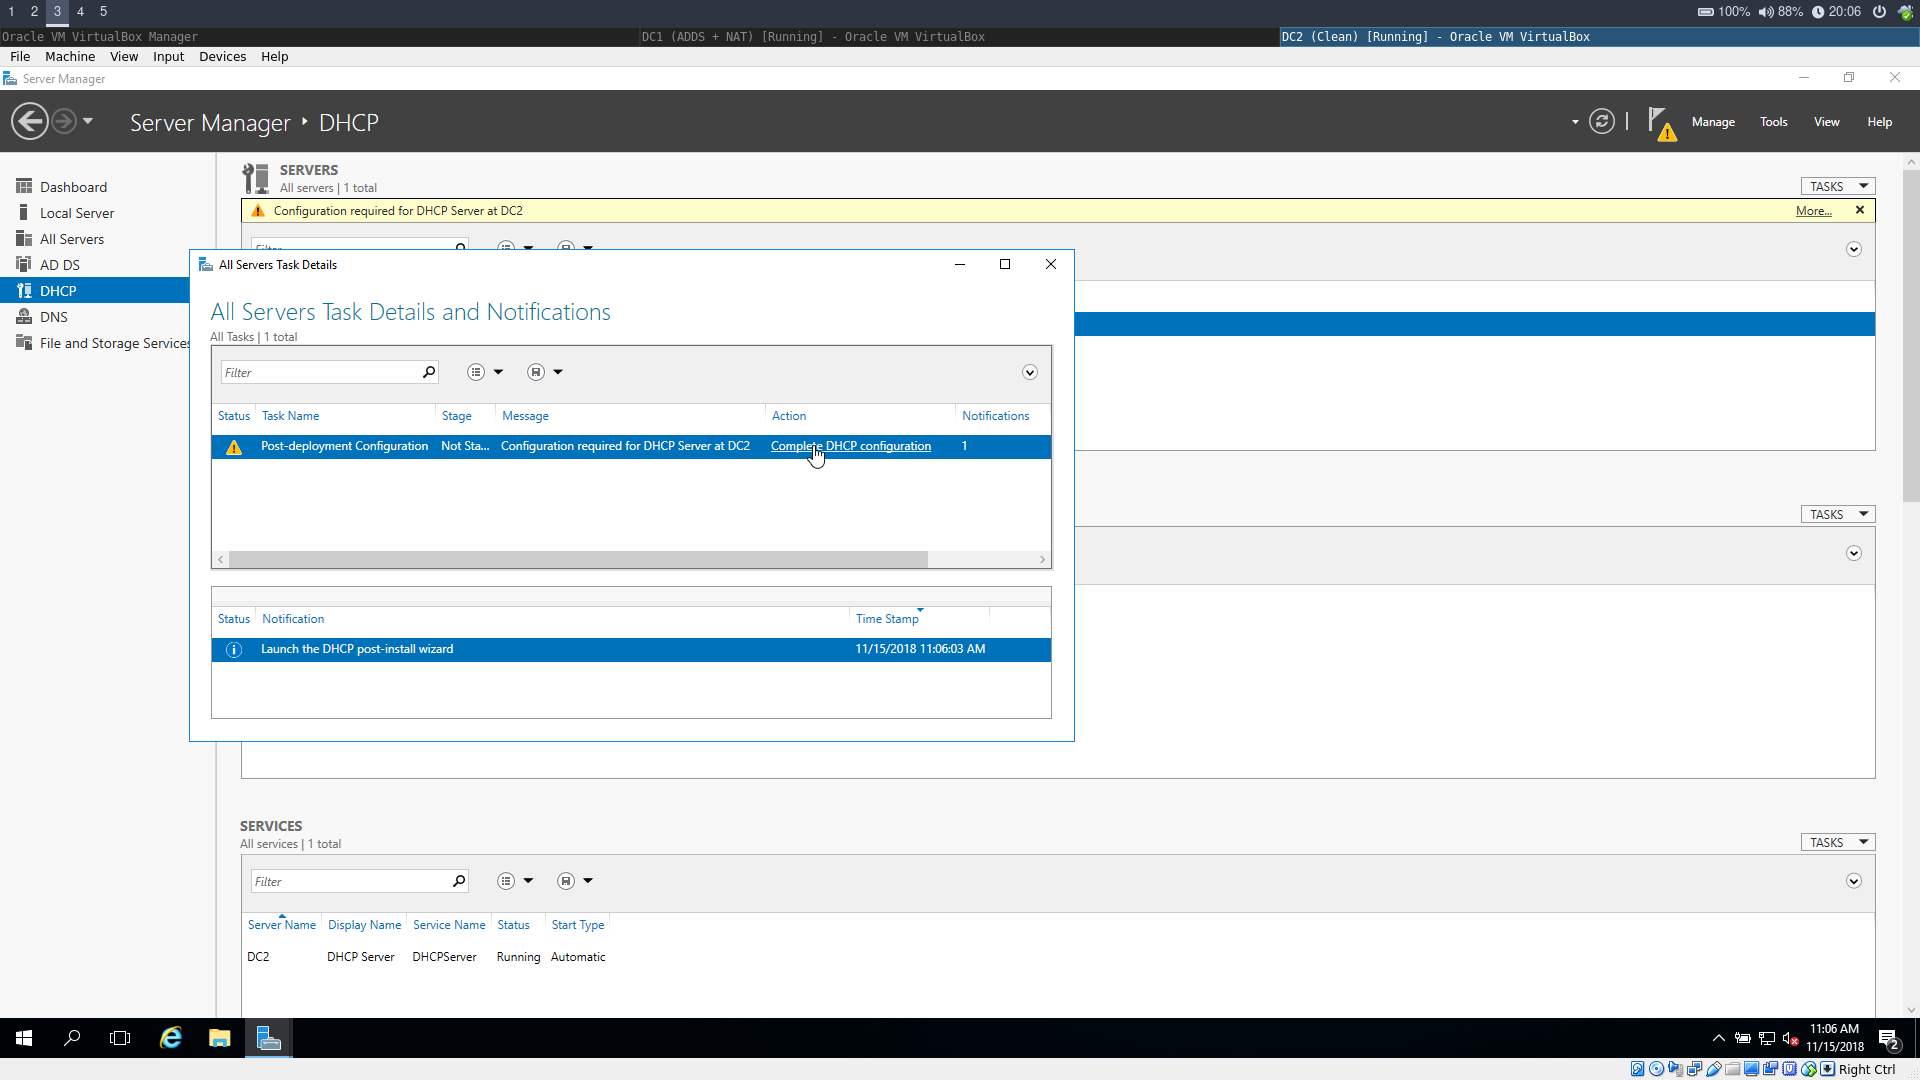
\includegraphics[width=15cm]{Pictures/DC2/DHCP/1542308778.png}
	
	Start de initiële configuratie.
\end{center}
\begin{center}
	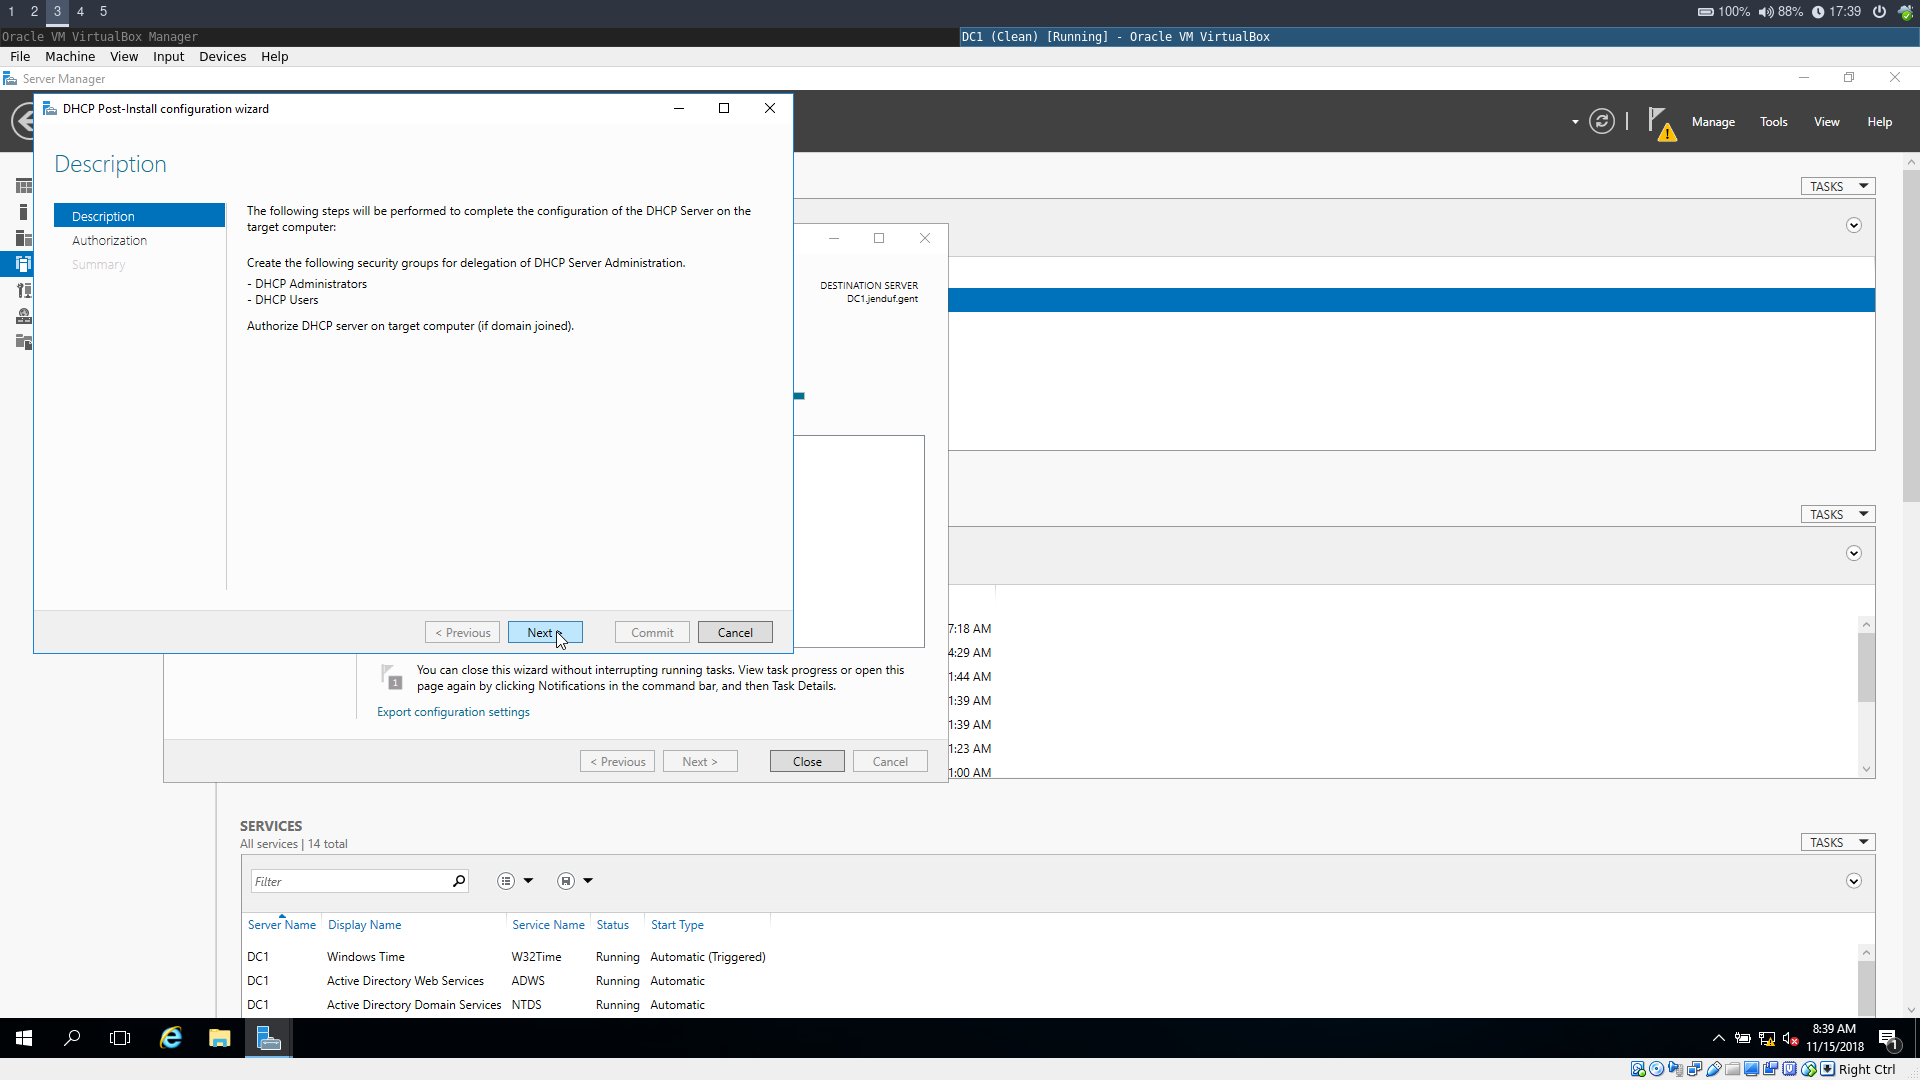
\includegraphics[width=15cm]{Pictures/DC2/DHCP/1542299964.png}
\end{center}
\begin{center}
	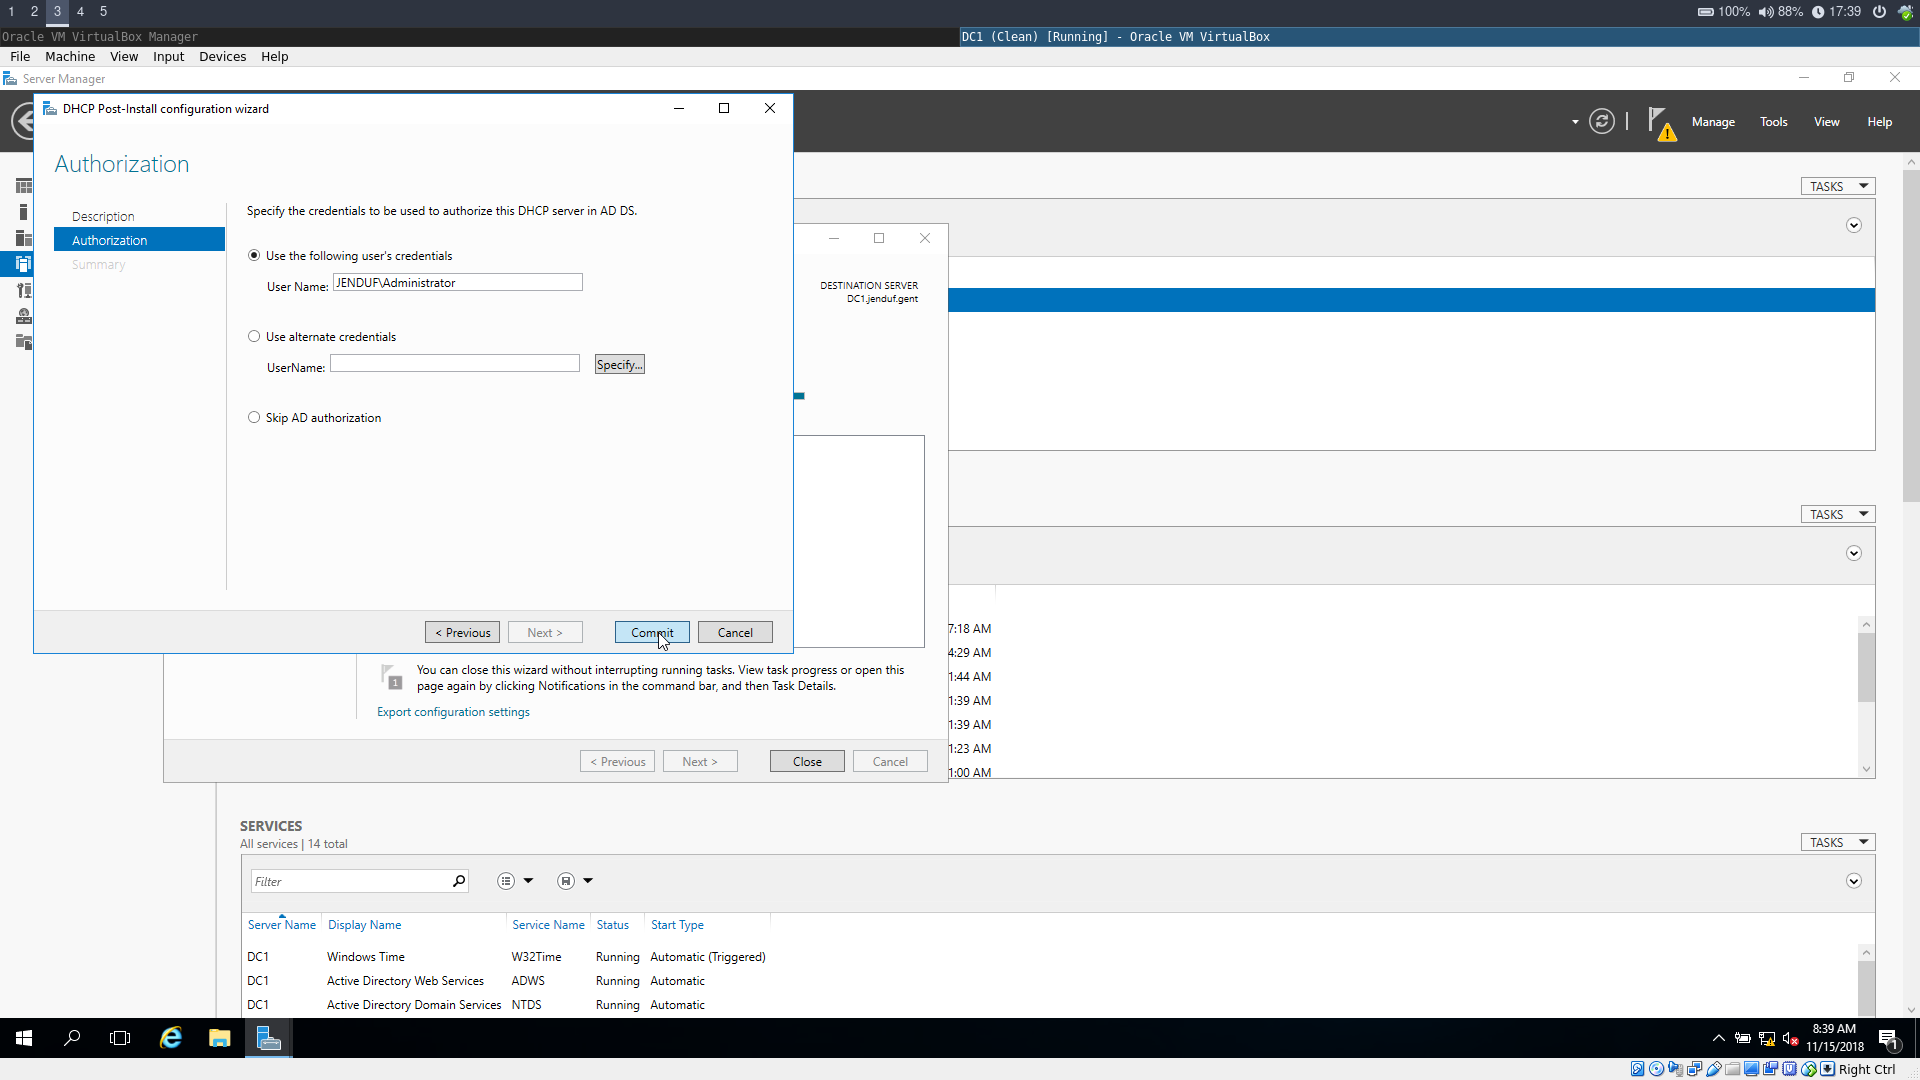
\includegraphics[width=15cm]{Pictures/DC2/DHCP/1542299973.png}
\end{center}
\begin{center}
	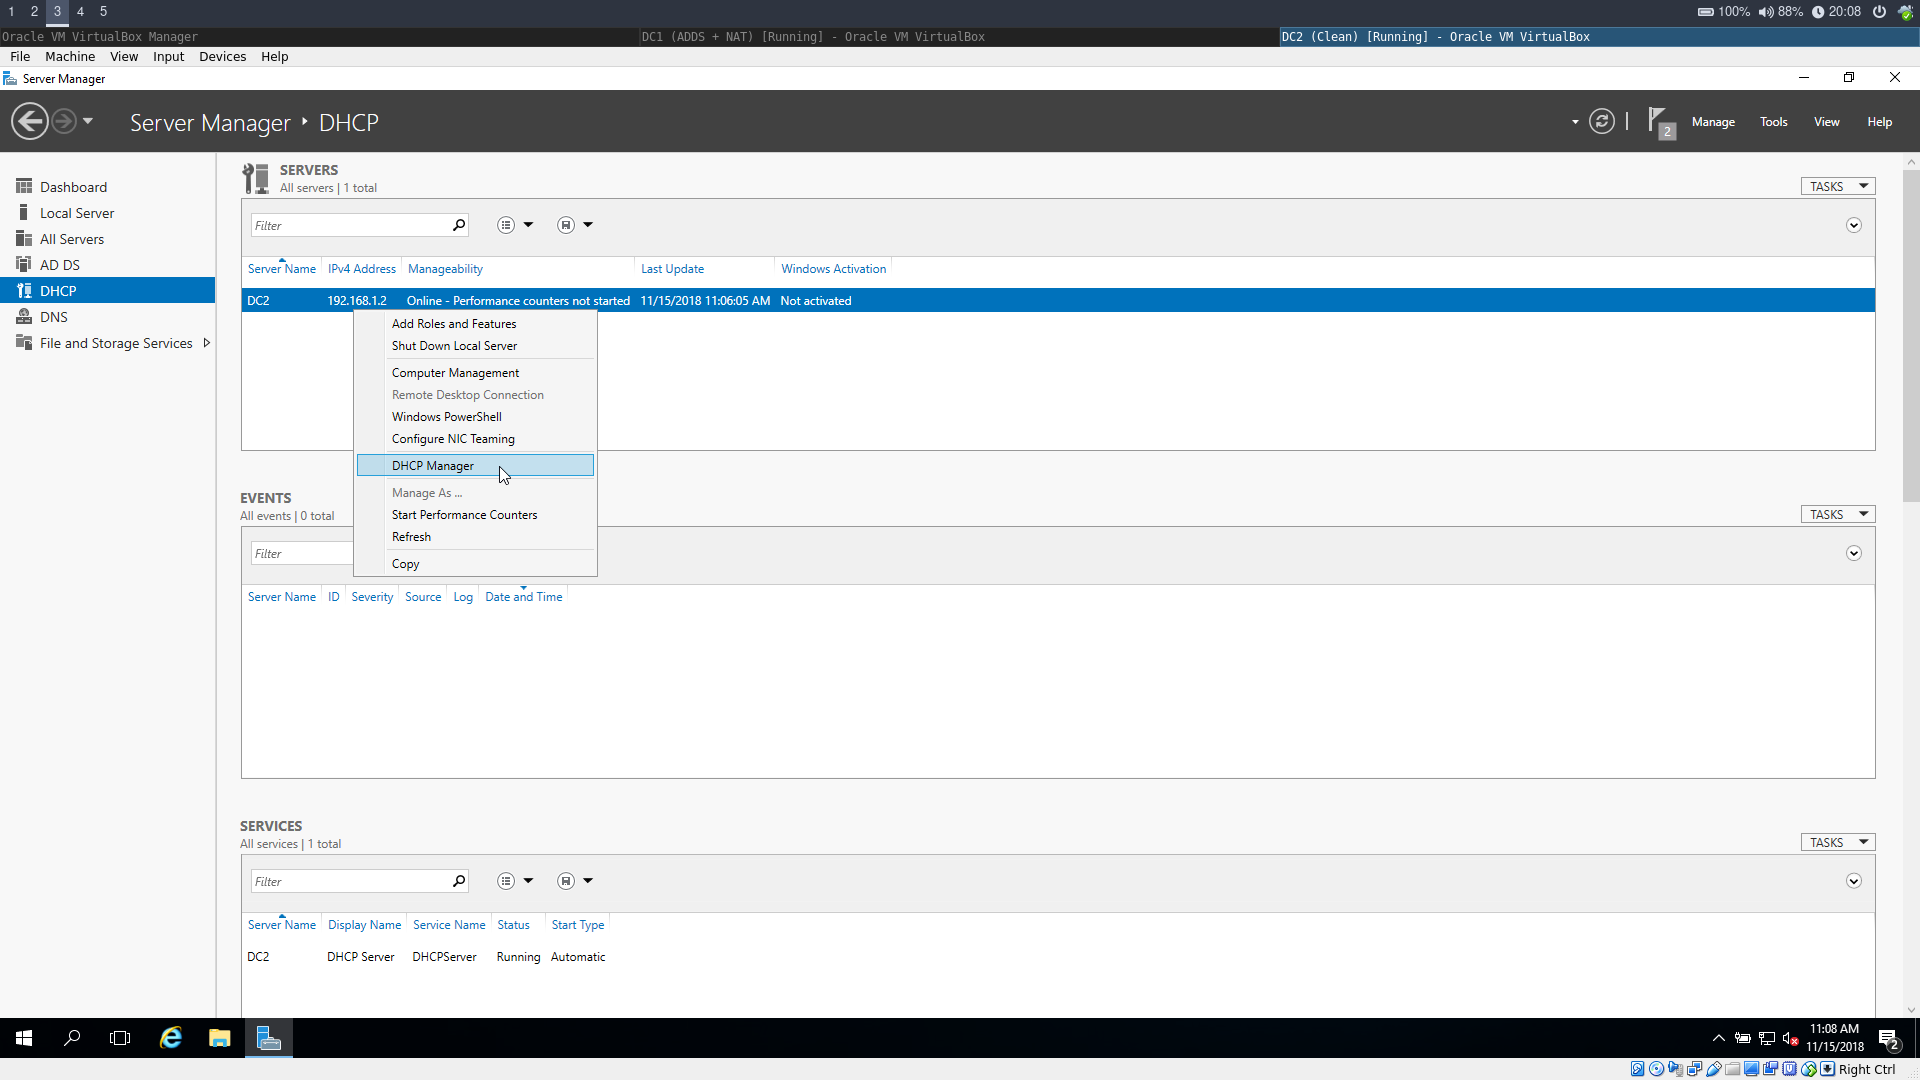
\includegraphics[width=15cm]{Pictures/DC2/DHCP/1542308921.png}
	
	Open de DHCP Manager.
\end{center}
\begin{center}
	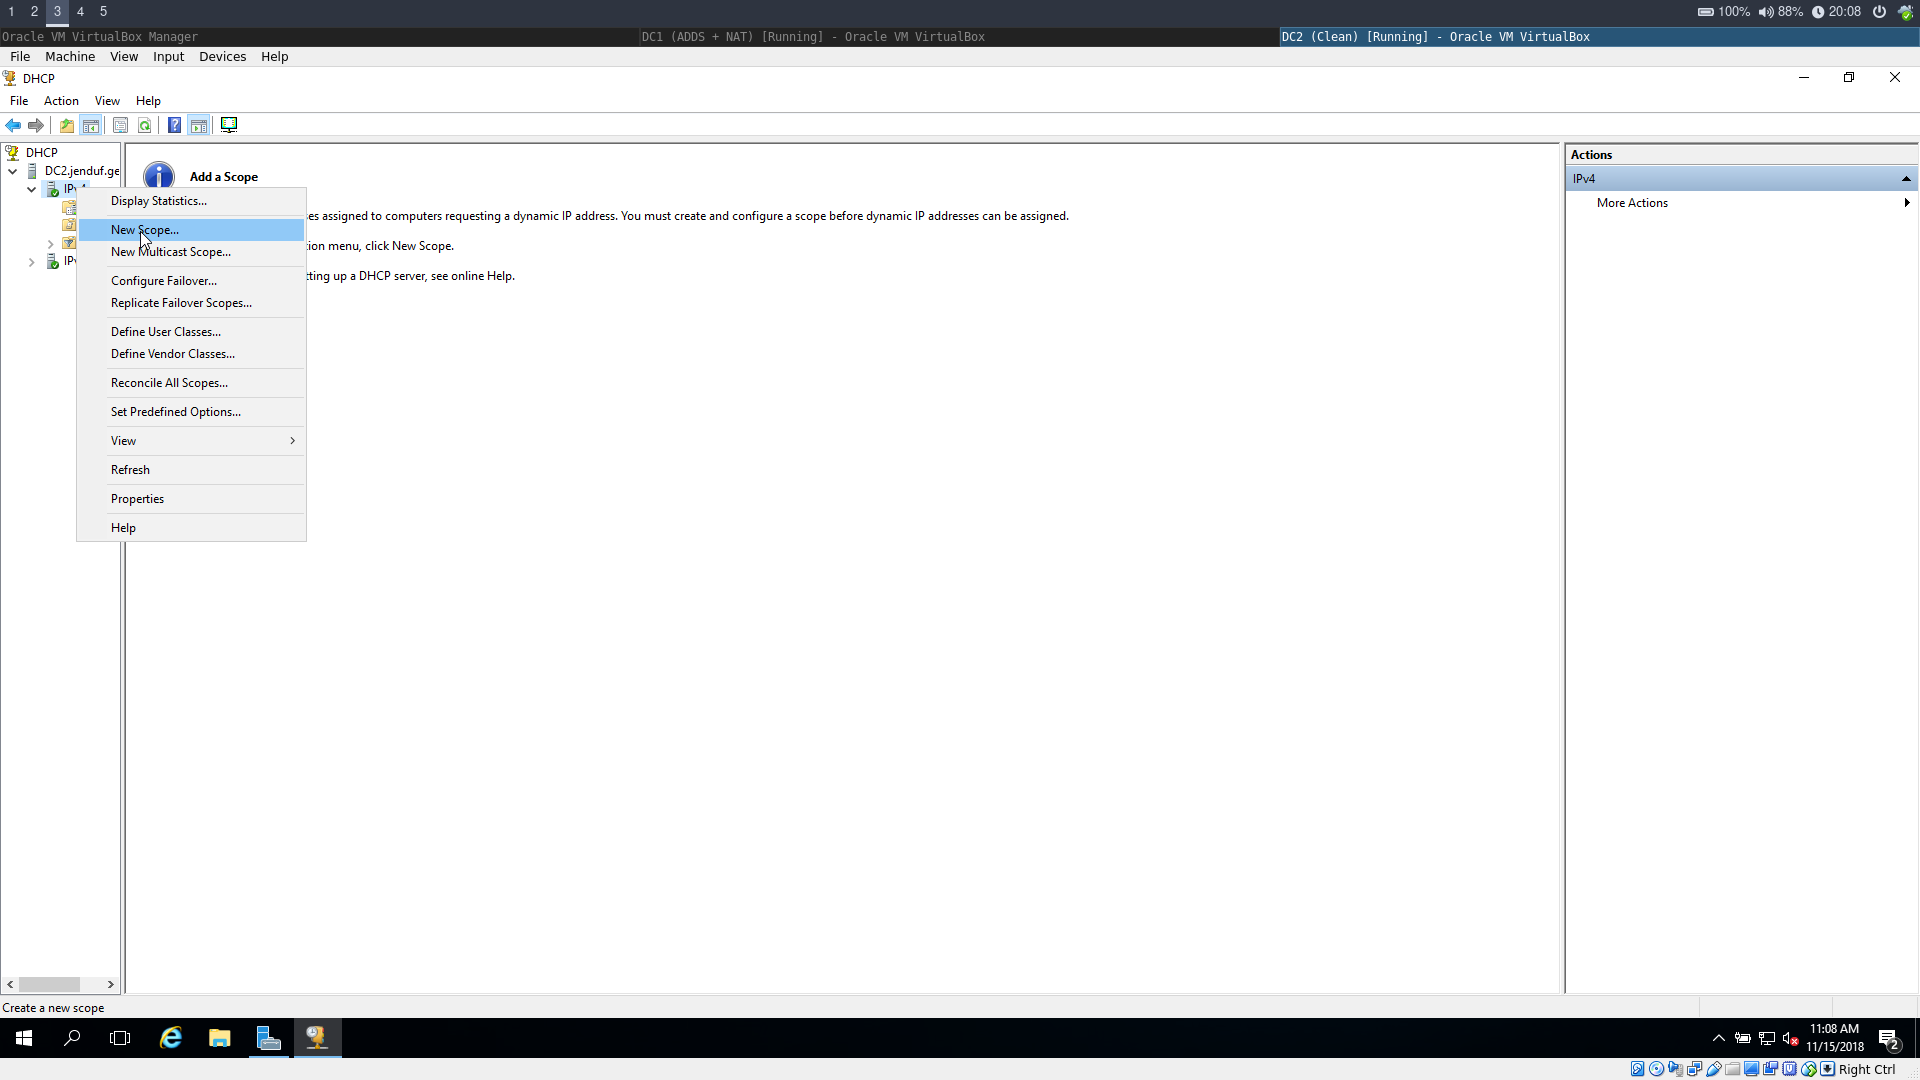
\includegraphics[width=15cm]{Pictures/DC2/DHCP/1542308937.png}
	
	Initialiseer een nieuwe scope op de DHCP Server.
\end{center}
\begin{center}
	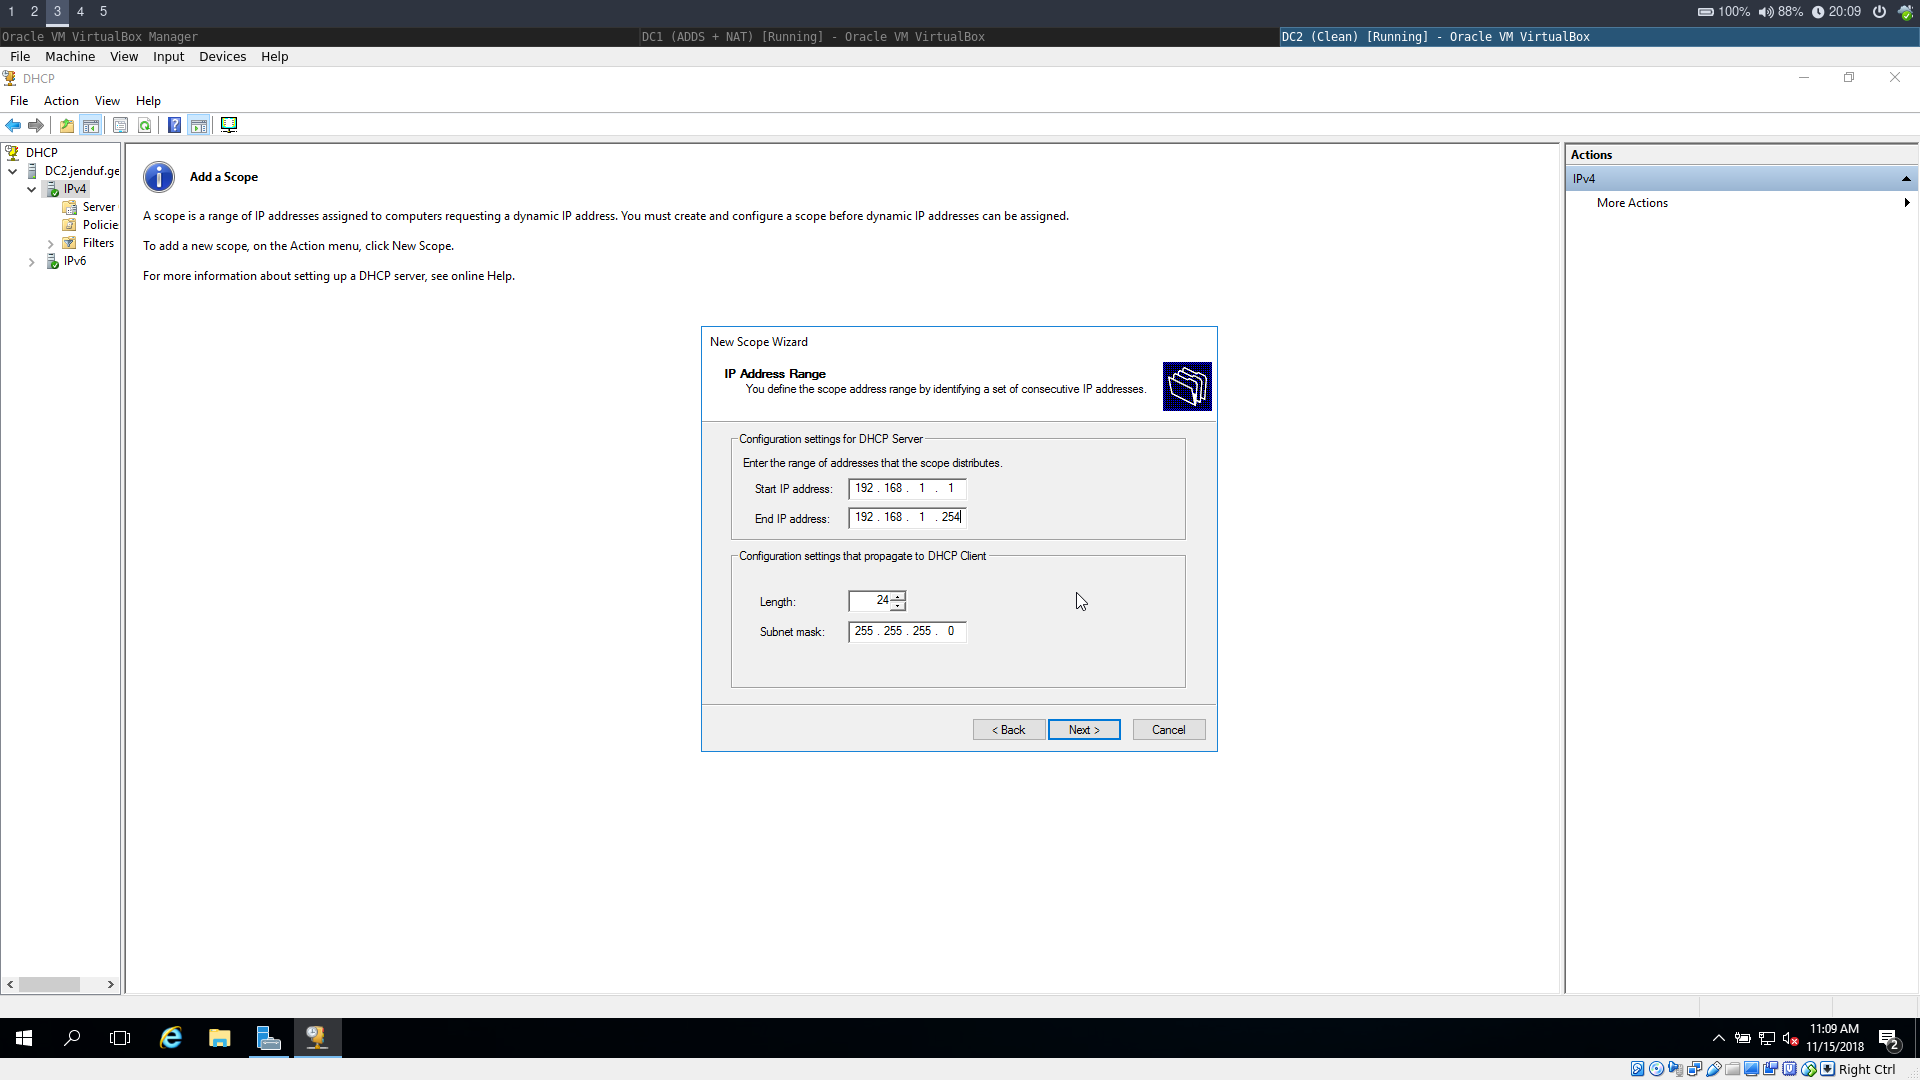
\includegraphics[width=15cm]{Pictures/DC2/DHCP/1542308958.png}
	Geef het IP bereik in van de DHCP Server.
\end{center}
\begin{center}
	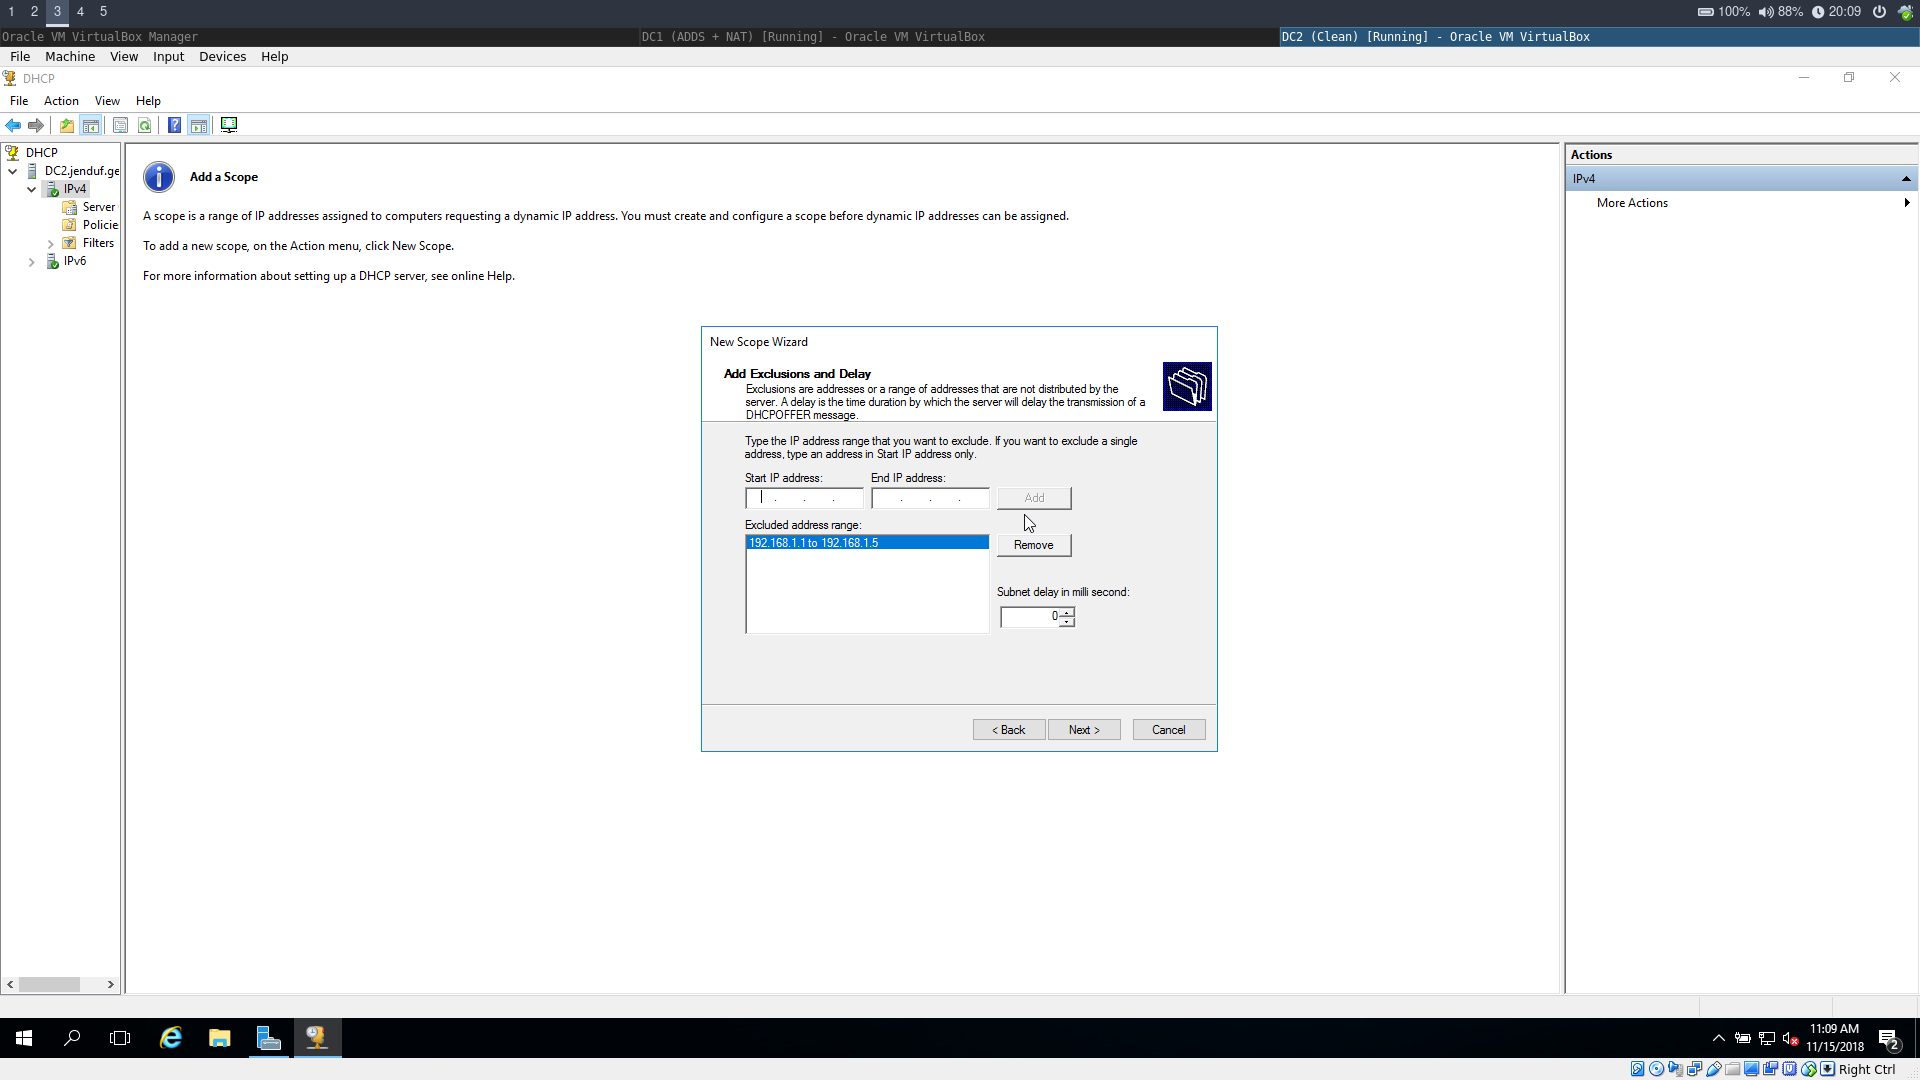
\includegraphics[width=15cm]{Pictures/DC2/DHCP/1542308975.png}
	
	Voeg de IP uitsluitingen uit aan de DHCP Server.
\end{center}
\begin{center}
	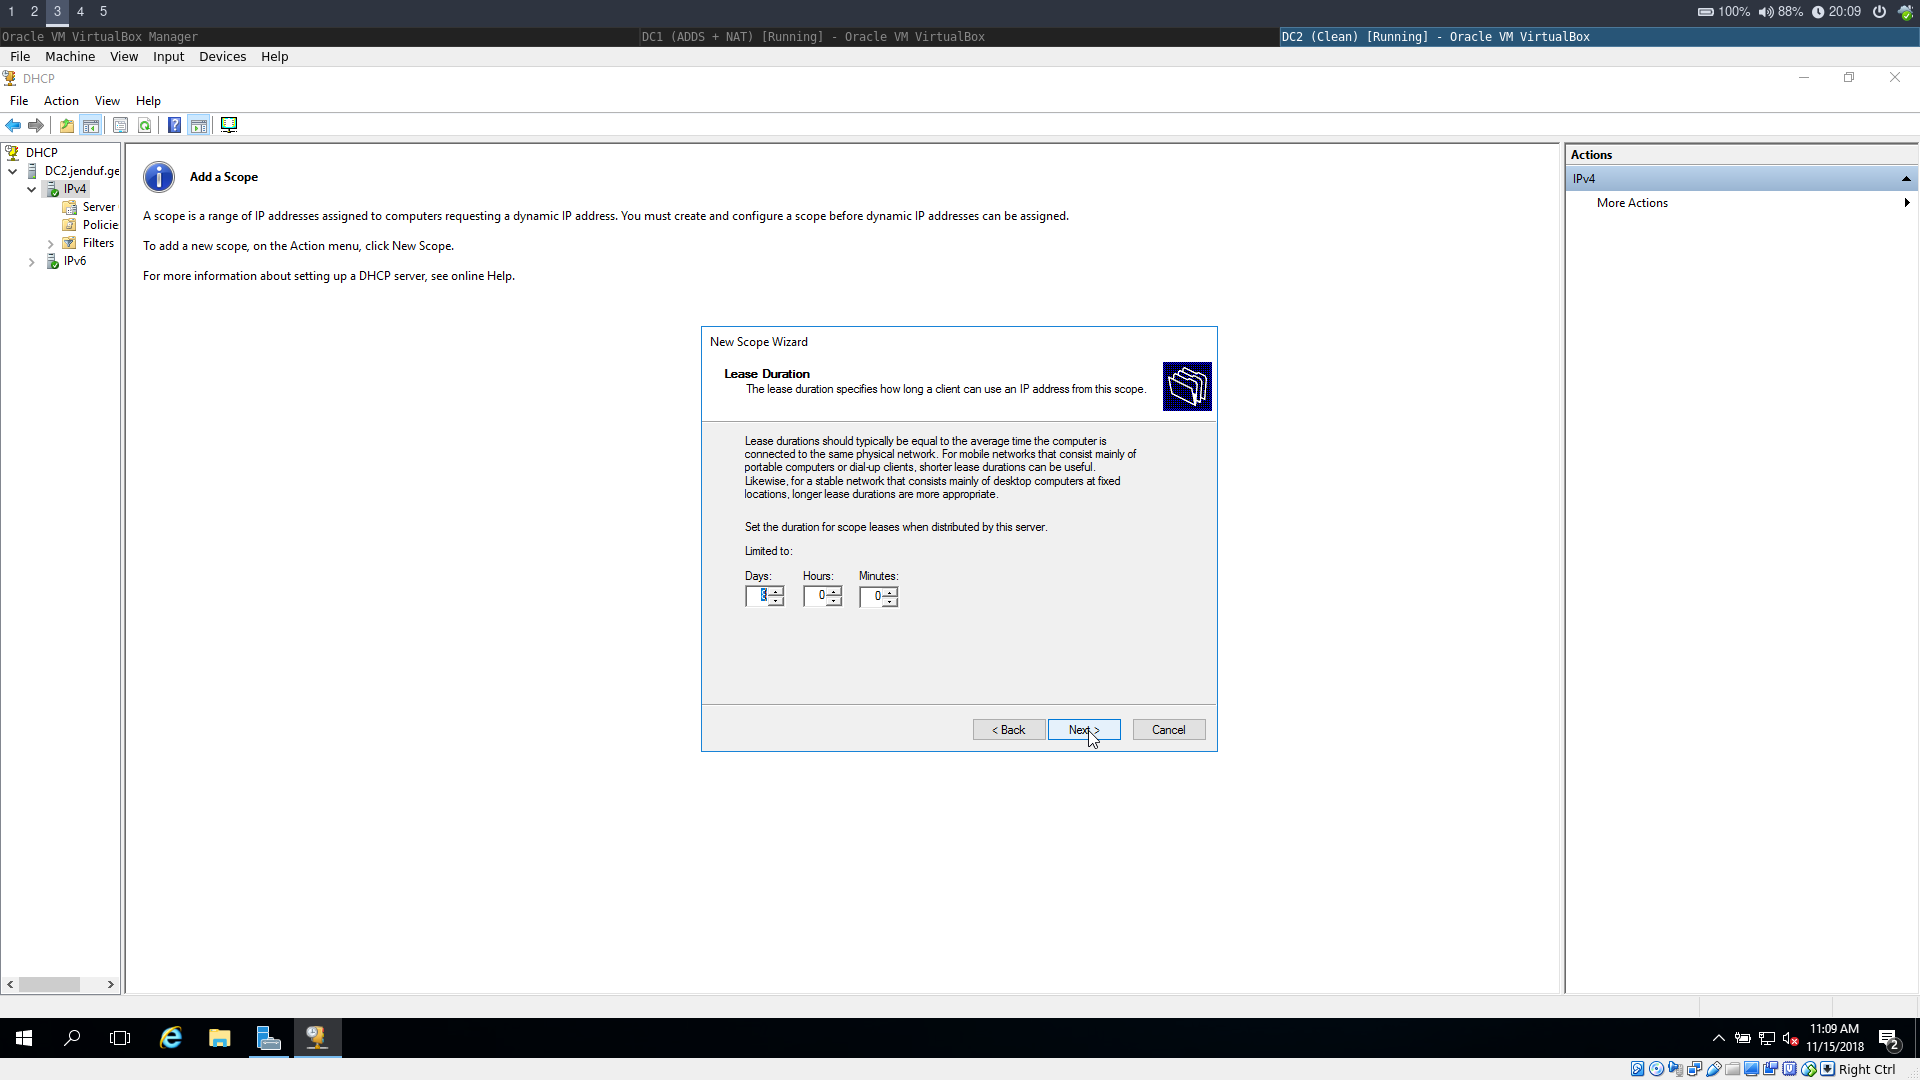
\includegraphics[width=15cm]{Pictures/DC2/DHCP/1542308991.png}
	
	Stel de levensduur in op 8 uur.
\end{center}
\begin{center}
	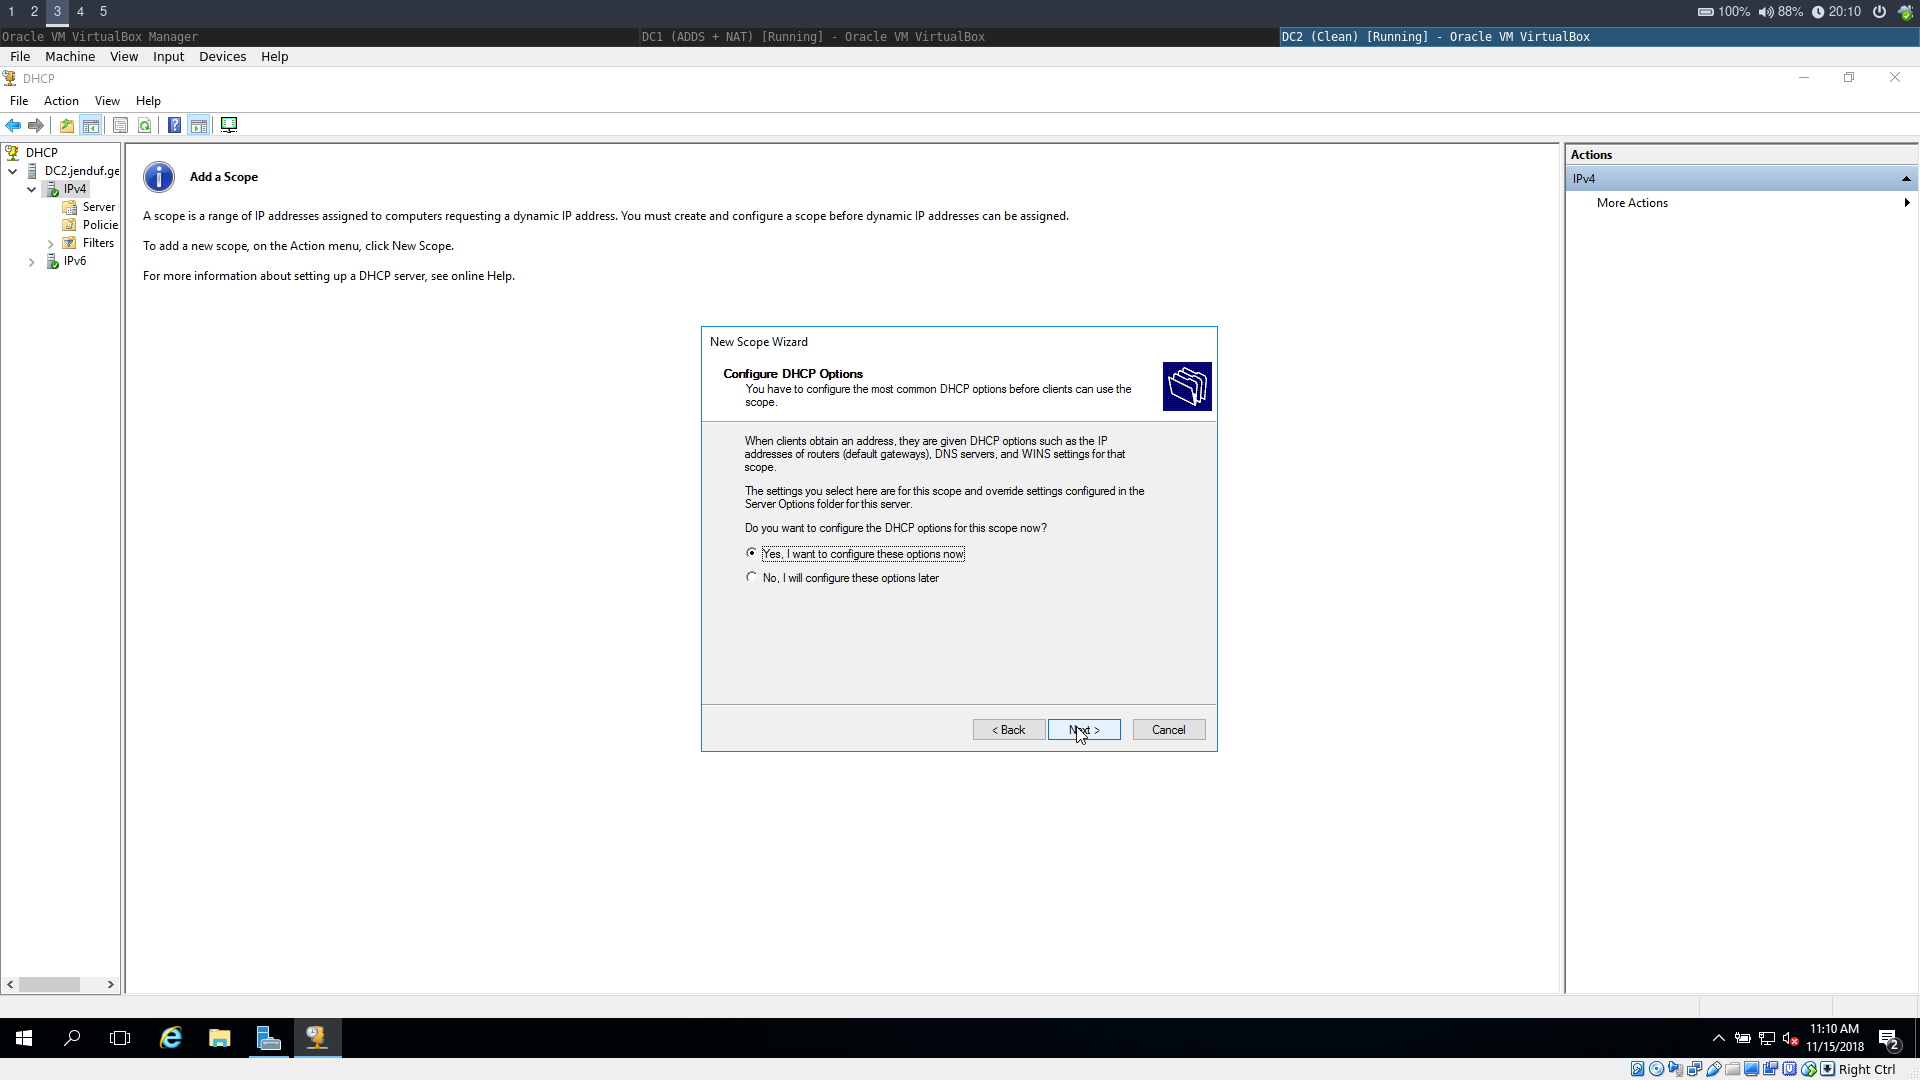
\includegraphics[width=15cm]{Pictures/DC2/DHCP/1542309046.png}
	
	Configureer de opties meteen.
\end{center}
\begin{center}
	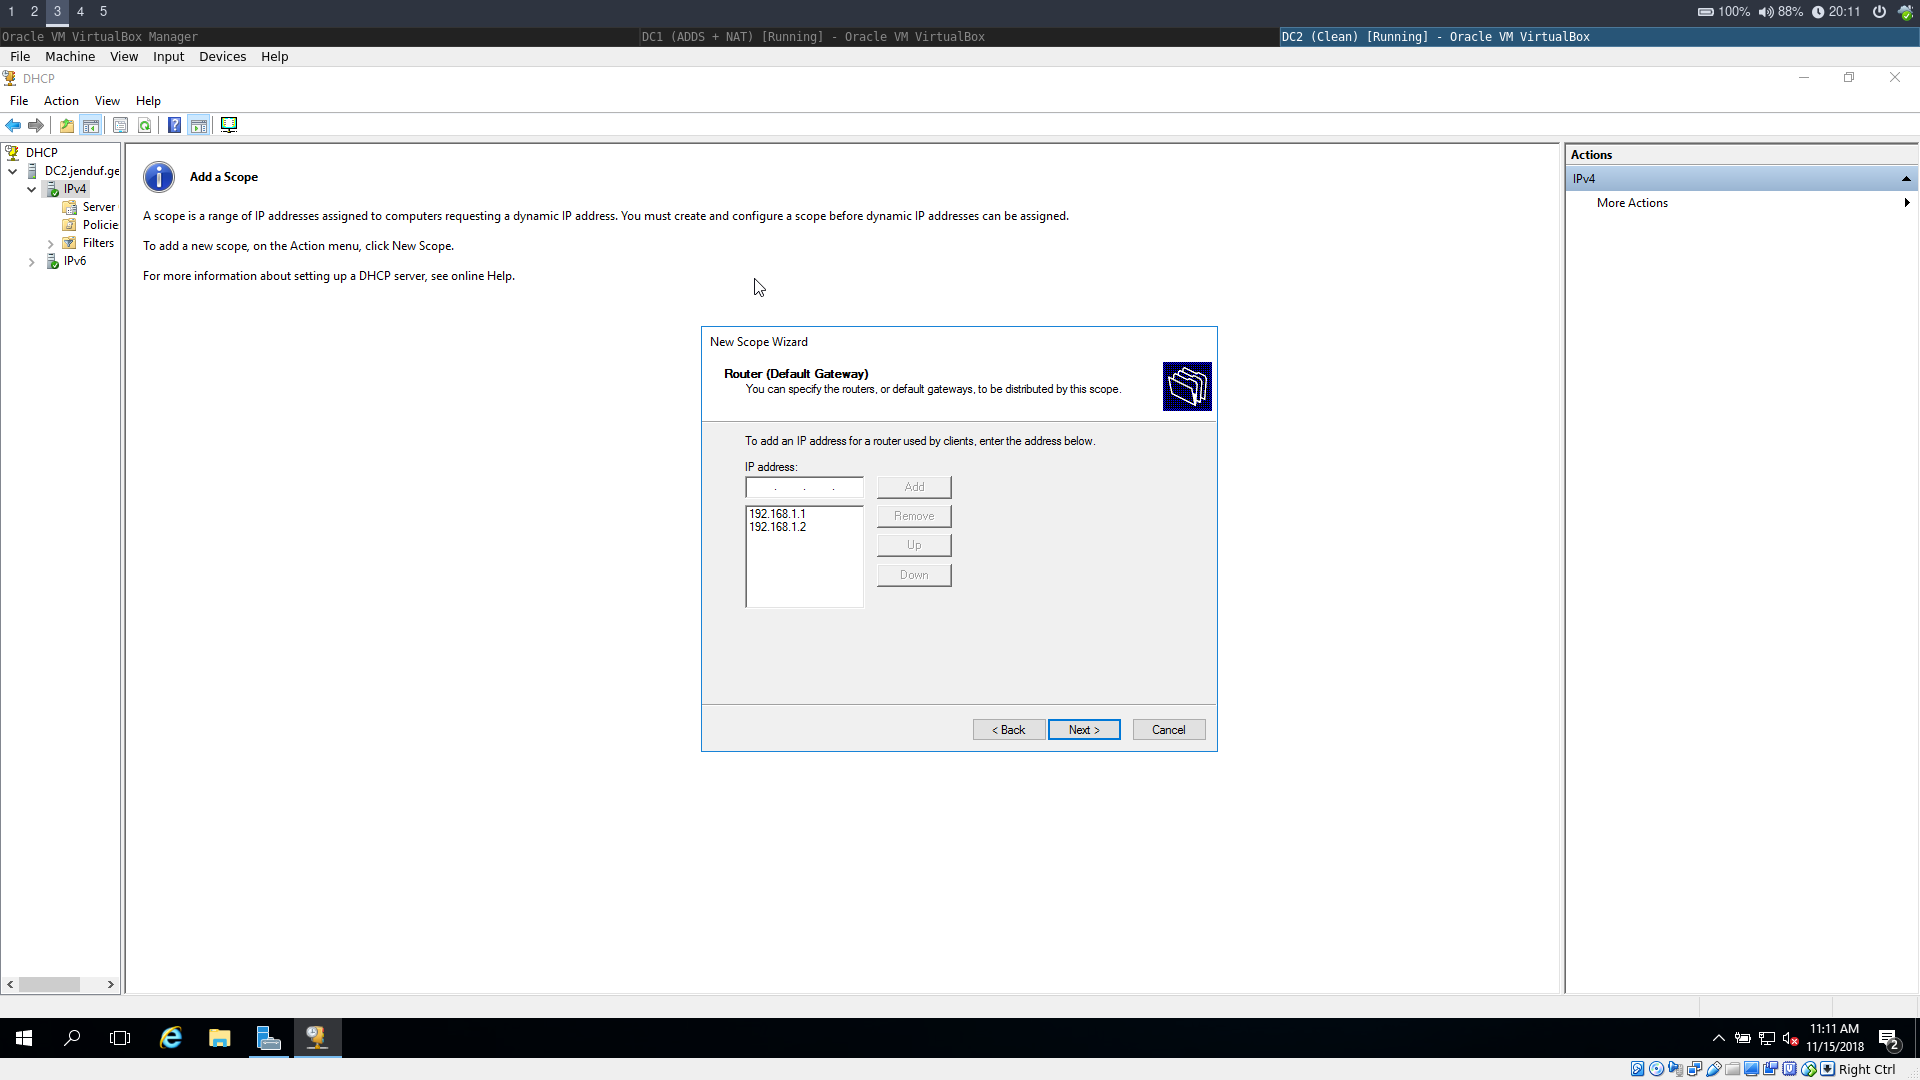
\includegraphics[width=15cm]{Pictures/DC2/DHCP/1542309061.png}
	
	Voeg het IP van DC1 en DC2 toe als Router.
\end{center}
\begin{center}
	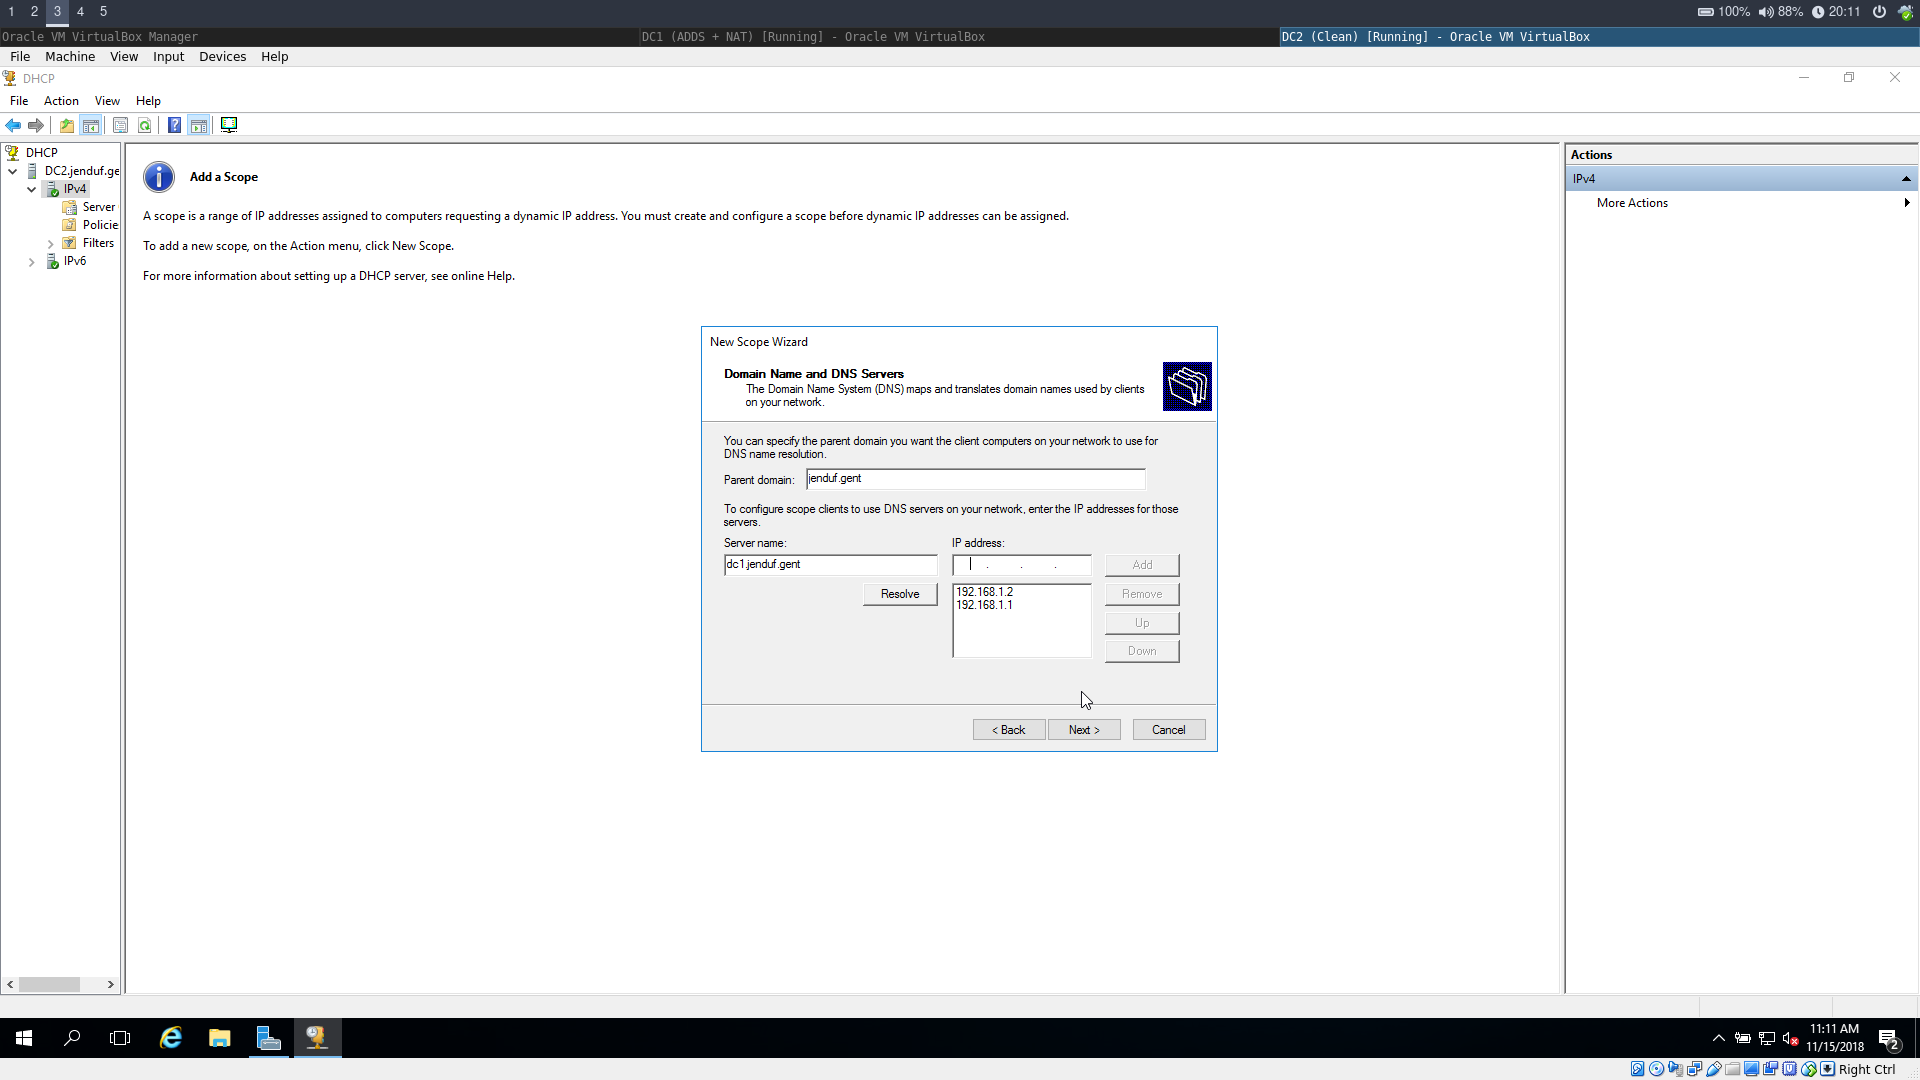
\includegraphics[width=15cm]{Pictures/DC2/DHCP/1542309102.png}
	
		Voeg het IP van DC1 en DC2 toe als DNS.
\end{center}
\begin{center}
	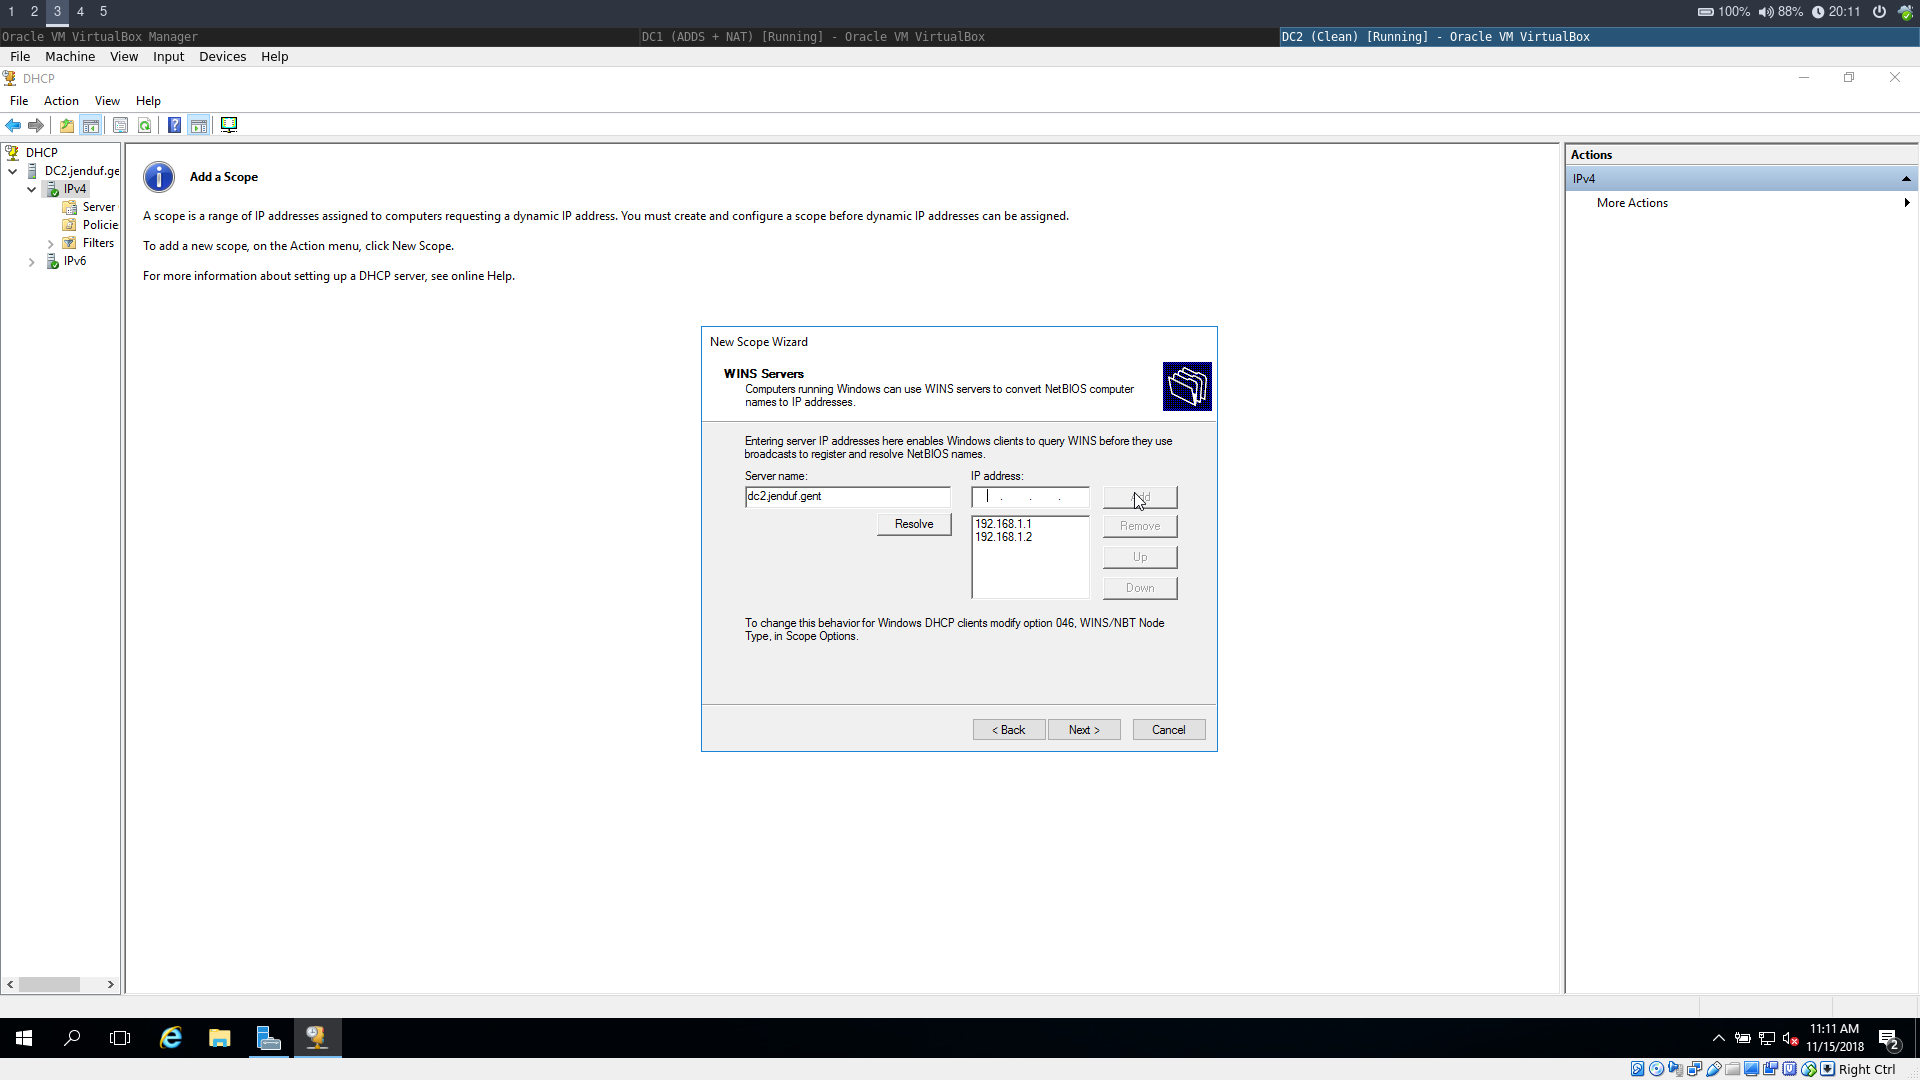
\includegraphics[width=15cm]{Pictures/DC2/DHCP/1542309120.png}
	
		Voeg het IP van DC1 en DC2 toe als WINS Server.
\end{center}
\begin{center}
	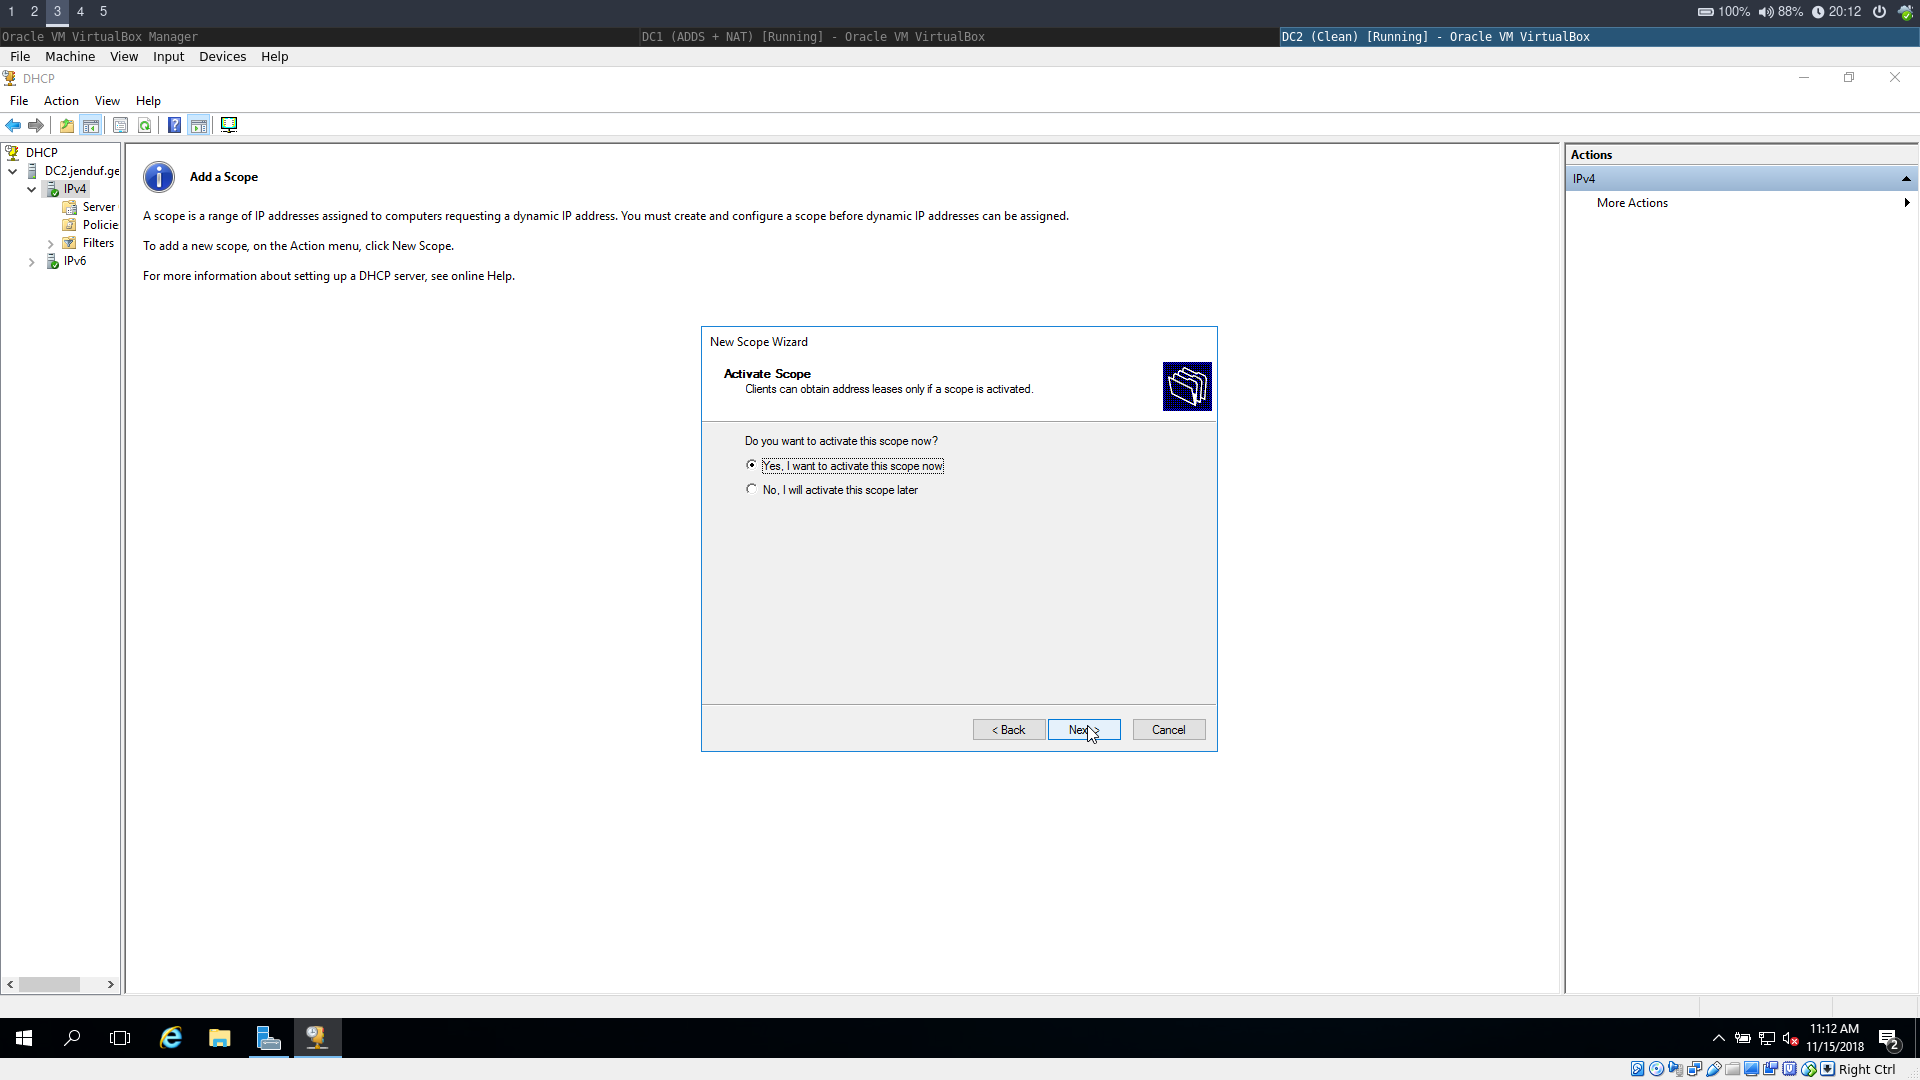
\includegraphics[width=15cm]{Pictures/DC2/DHCP/1542309123.png}
	
	Activeer de scope onmiddelijk.
\end{center}


\section{Configuratie DNS}
De DNS-service werd automatisch geïnstalleerd met de ADDS.

\clearpage

\section{Powershell}

Script 1:

\begin{verbatim}
	#Activeer PS
	Set-ExecutionPolicy Unrestricted
	#Declaring variables
	$hostname = "DC2"
	
	#Computer naam wijzigen
	Rename-Computer -ComputerName $env:COMPUTERNAME  -newName $hostname -Force -Restart
\end{verbatim}

Script 2:

\begin{verbatim}
	#Declaring variables
	$domainname = "jenduf.gent"
	
	#IP-adres en default gateway wijzigen
	New-NetIPAddress -InterfaceAlias "Ethernet" -IPAddress 192.168.1.2 
	-DefaultGateway 192.168.1.1 -PrefixLength 24
	Set-DnsClientServerAddress -InterfaceAlias "Ethernet" -ServerAddresses 192.168.1.1, 192.18.1.2
	
	#Firewall uitschakelen
	Set-NetFirewallProfile -Profile Domain,Public,Private -Enabled False
	
	#JoinDomain
	Write-Host 'Trying to join domain jenduf.gent'
	$DomainName = "jenduf.gent"
	$SafeModeAdministratorPassword = "Project2018" | ConvertTo-SecureString -AsPlainText -Force
	$domain = "jensduf"
	$joindomainuser = "Administrator"
	$credential = New-Object System.Management.Automation.PSCredential
	($joindomainuser,$SafeModeAdministratorPassword)
	Add-Computer -DomainName $DomainName -Credential $credential
	
	#DC en DNS installeren en domeinnaam instellen
	Install-WindowsFeature AD-Domain-Services -IncludeManagementTools
	Install-ADDSDomainController -DomainName $domainname -SafeModeAdministratorPassword:
	(ConvertTo-SecureString -String "Admin2018" -AsPlainText -Force) -Force
	
	#Server opnieuw opstarten
	Restart-computer
\end{verbatim}
\end{document}